\documentclass[11pt,a4paper]{article}

% ------------------------------------------------------------------ paquetes
\usepackage[utf8]{inputenc}
\usepackage[T1]{fontenc}
\usepackage{lmodern}
\usepackage[spanish,es-tabla,es-nodecimaldot]{babel}
\usepackage[margin=2.2cm]{geometry}
\usepackage{graphicx}
\usepackage{booktabs}
\usepackage{longtable}
\usepackage{float}
\usepackage{array}
\usepackage{amsmath}
\usepackage{enumitem}
\usepackage[table]{xcolor}
\usepackage[font=small,labelfont=bf,skip=4pt]{caption}
\usepackage{tcolorbox}
\usepackage{fancyhdr}
\usepackage[hidelinks]{hyperref}

\graphicspath{{../figures/eda/}}
\definecolor{ame}{HTML}{1C5CAB}
\definecolor{hip}{HTML}{EB6834}
\DeclareRobustCommand{\col}[1]{\texttt{\detokenize{#1}}}
\newtcolorbox{historia}[1][]{colback=ame!5,colframe=ame,boxrule=0.6pt,arc=2pt,left=6pt,right=6pt,top=4pt,bottom=4pt,title={#1},fonttitle=\bfseries\small}
\newtcolorbox{hipotesis}[1][]{colback=hip!6,colframe=hip,boxrule=0.6pt,arc=2pt,left=6pt,right=6pt,top=4pt,bottom=4pt,title={#1},fonttitle=\bfseries\small}
\setlist{itemsep=2pt,topsep=3pt}
\renewcommand{\arraystretch}{1.12}
\pagestyle{fancy}\fancyhf{}
\lhead{\small ISAC Hackathon 2026 · Club América}\rhead{\small Análisis exploratorio de datos}
\cfoot{\small\thepage}

\title{\textbf{¿Qué historia cuentan los datos?}\\[4pt]
\large Análisis exploratorio (EDA) de los datos StatsBomb del Club América, 2021--2026\\[2pt]
\normalsize Reto ISAC 2026: \emph{La historia de un entrenador a través de los datos}}
\author{Equipo ISAC-Hackathon-America}
\date{Septiembre de 2026}

\begin{document}
\maketitle
\thispagestyle{empty}

\begin{abstract}
\noindent Este documento es la primera fase del proyecto: \textbf{entender los datos antes de concluir}. Se analizan 222 partidos de Liga MX del Club América (julio 2021 -- septiembre 2026) con datos de eventos StatsBomb y StatsBomb 360, que abarcan cinco entrenadores: Santiago Solari, Fernando Ortiz, André Jardine (129 partidos), Diego Cervantes (interino) y Jorge Almada. Para cada una de las seis tablas se documenta qué significa cada columna, su calidad, su distribución y sus relaciones con otras variables; después se cruzan las métricas con el contexto que pide el reto (tiempo, entrenador, localía, nivel del rival, fase del torneo y marcador). El análisis es \emph{descriptivo}: no se prueban hipótesis ni se controla por rival. Aun así, los datos ya esbozan una historia coherente --- la posesión no distingue a los entrenadores, pero la \emph{intensidad de la presión}, la \emph{precisión} y la \emph{adaptación al contexto} sí --- que se formula como diez hipótesis a contrastar en la fase de análisis.
\end{abstract}

\tableofcontents
\newpage

% =====================================================================
\section{Introducción}
% =====================================================================
\subsection{El reto}
El reto ISAC 2026 pide construir, \emph{únicamente a partir de los datos}, una narrativa que permita a alguien que no vio los partidos entender cómo juega un equipo y qué ideas tácticas definen a su entrenador. La pregunta central es:

\begin{historia}[Pregunta central del reto]
¿Cuáles son los principios que definen al equipo en fase ofensiva y defensiva, cómo se manifiestan estos patrones a lo largo del tiempo, y de qué manera el entrenador ajusta su comportamiento en función del contexto del partido (rival, marcador, localía o momento del juego)?
\end{historia}

Los componentes esperados son: estilo de juego (construcción, progresión, generación de ocasiones; presión, organización defensiva, transiciones), consistencia y variabilidad, uso de jugadores, balón parado ofensivo y defensivo, evidencia cuantitativa (xG, OBV, pases progresivos, presión, field tilt) y un marco analítico explícito.

\subsection{Objetivo de este documento}
Antes de modelar cualquier cosa es necesario saber qué información existe, qué significa, qué tan confiable es y qué relaciones muestra. Los objetivos de este EDA son:
\begin{enumerate}
  \item \textbf{Inventariar y describir} las seis tablas (granularidad, tipos, semántica de cada columna).
  \item \textbf{Evaluar la calidad} de los datos (faltantes, anomalías, coherencia interna).
  \item \textbf{Describir distribuciones} univariadas (numéricas y categóricas) y \textbf{relaciones} bivariadas (correlación de Spearman, V de Cramér).
  \item \textbf{Cruzar con el contexto} que pide el reto (tiempo, entrenador, localía, rival, fase, marcador).
  \item \textbf{Formular hipótesis} y \textbf{definiciones preliminares} para el marco analítico.
\end{enumerate}
No se extraen conclusiones: toda diferencia reportada es descriptiva y está sujeta a validación.

\subsection{Cómo leer este reporte}
Las Secciones~\ref{sec:datos}--\ref{sec:calidad} describen los datos y su calidad; la~\ref{sec:univariado} describe cada tabla columna por columna; la~\ref{sec:relaciones} analiza relaciones entre variables; la~\ref{sec:contexto} cruza con el contexto; la~\ref{sec:historia} sintetiza la historia y las hipótesis; la~\ref{sec:marco} traduce lo aprendido en definiciones para el marco analítico. El Apéndice~\ref{app:dic} contiene el diccionario completo de columnas.

% =====================================================================
\section{Datos}\label{sec:datos}
% =====================================================================
\subsection{Fuente y adquisición}
Los datos provienen de la API privada de StatsBomb (Hudl), con credenciales de uso exclusivo para la competencia. La descarga se automatizó (notebook \col{01_descarga_datos.ipynb}, módulo \col{src/sb_client.py}) con la librería \col{statsbombpy}: para cada partido del América con estado \col{available} se descargan eventos, frames 360, alineaciones y estadísticas agregadas de jugador y equipo, y se guardan en Parquet por partido (proceso reanudable). Las credenciales y los datos están excluidos del control de versiones.

Las credenciales dan acceso a Liga MX (competición 73, seis temporadas con 360) y Liga MX Femenil (tres temporadas, sin 360). Este proyecto usa \textbf{Liga MX varonil}. Una ``temporada'' StatsBomb agrupa Apertura (julio--diciembre) y Clausura (enero--mayo), incluidas las liguillas.

\subsection{Alcance}
\begin{table}[H]
\centering
\small
\caption{Inventario de tablas descargadas.}
\label{tab:inventario}
\resizebox{\ifdim\width>\linewidth\linewidth\else\width\fi}{!}{%
\begin{tabular}{llrrr}
\toprule
\textbf{Tabla} & \textbf{Granularidad (1 fila =)} & \textbf{Filas} & \textbf{Columnas} & \textbf{Partidos} \\
\midrule
matches & 1 partido del América & 222 & 69 & 222 \\
events & 1 evento (ambos equipos) & 736,829 & 162 & 222 \\
team\_match\_stats & 1 equipo x partido & 442 & 216 & 221 \\
player\_match\_stats & 1 jugador x partido & 6,870 & 187 & 222 \\
lineups & 1 convocado x partido & 9,317 & 25 & 222 \\
frames360 & 1 jugador visible x evento & 8,925,818 & 8 & 221 \\
\bottomrule
\end{tabular}}
\end{table}
\begin{table}[H]
\centering
\small
\caption{Cobertura por temporada y entrenador.}
\label{tab:cobertura}
\resizebox{\ifdim\width>\linewidth\linewidth\else\width\fi}{!}{%
\begin{tabular}{lrrrll}
\toprule
\textbf{Temporada · entrenador} & \textbf{Jugados} & \textbf{Con eventos} & \textbf{Con 360} & \textbf{Desde} & \textbf{Hasta} \\
\midrule
2021/2022 · Ortiz & 13 & 13 & 13 & 2022-03-06 & 2022-05-23 \\
2021/2022 · Solari & 27 & 27 & 27 & 2021-07-23 & 2022-03-02 \\
2022/2023 · Ortiz & 42 & 42 & 42 & 2022-07-03 & 2023-05-22 \\
2023/2024 · Jardine & 46 & 46 & 46 & 2023-07-01 & 2024-05-27 \\
2024/2025 · Jardine & 45 & 45 & 45 & 2024-07-06 & 2025-05-26 \\
2024/2025 · Cervantes & 2 & 2 & 2 & 2025-01-11 & 2025-01-17 \\
2025/2026 · Jardine & 38 & 38 & 37 & 2025-07-12 & 2026-05-11 \\
2026/2027 · Almada & 9 & 9 & 9 & 2026-07-19 & 2026-09-28 \\
\bottomrule
\end{tabular}}
\end{table}

El América disputó 222 partidos con datos disponibles (más 8 programados de 2026/27). \textbf{André Jardine concentra el 58\% de la muestra} (129 partidos en tres temporadas y seis torneos), lo que lo convierte en el candidato natural a protagonista de la narrativa; los demás entrenadores funcionan como contraste (antes: Solari y Ortiz; después: Almada, con solo 9 partidos). Cervantes dirigió 2 partidos como interino y se excluye de las comparaciones.

\subsection{Sistema de coordenadas}
StatsBomb usa una cancha de $120\times80$ yardas. En cada evento, \textbf{el equipo que ejecuta la acción ataca de izquierda a derecha}: $x=0$ es su propia portería y $x=120$ la rival; $y$ va de 0 a 80 (banda a banda). El último tercio es $x\geq80$ y el área rival $x\geq102,\ 18\leq y\leq62$. Esto permite comparar acciones de ambos equipos sin reorientar.

% =====================================================================
\section{Metodología del EDA}\label{sec:metodologia}
% =====================================================================
\paragraph{Clasificación de columnas.} Cada columna se asigna automáticamente a un tipo analítico: \emph{id}, \emph{numérica}, \emph{booleana}, \emph{categórica} (hasta 60 categorías), \emph{categórica de alta cardinalidad}, \emph{fecha}, \emph{coordenadas} (listas $[x,y]$, que se expanden a \col{_x} y \col{_y}) o \emph{JSON} (estructuras anidadas).

\paragraph{Perfiles.} Numéricas: conteo, \% de nulos, mínimo, percentiles 5/25/50/75/95, media, máximo, desviación estándar, moda y su frecuencia, \% de ceros y asimetría. Categóricas: número de categorías, moda, \% de cada categoría y \% acumulado del top-$k$. Booleanas: \% de \texttt{True}.

\paragraph{Perfil condicionado al tipo de evento.} Las columnas específicas (\col{pass_*}, \col{shot_*}, \col{duel_*}, \ldots) solo existen en su tipo de evento; perfilarlas sobre toda la tabla daría $>95\%$ de nulos sin significado. Por eso cada una se describe \textbf{solo sobre las filas de su tipo}.

\paragraph{Relaciones.} Entre numéricas se usa la \textbf{correlación de Spearman} ($\rho$), robusta a la fuerte asimetría de xG, OBV y conteos. Entre categóricas se usa la \textbf{V de Cramér} con corrección de sesgo (0 = independencia, 1 = asociación total).

\paragraph{Métricas derivadas (definiciones preliminares).}
\begin{itemize}
  \item \textbf{Field tilt}: pases del América en su último tercio ($x\geq80$) entre los pases de ambos equipos en su respectivo último tercio.
  \item \textbf{Pase progresivo}: pase completo de juego abierto (\col{pass_type} nulo) que reduce al menos 25\% la distancia a la portería rival y termina en $x\geq48$.
  \item \textbf{Altura de juego y de presión}: $x$ medio de los pases del América y de sus presiones.
  \item \textbf{Precisión de pase}: \col{successful_passes}/\col{passes} (ver anomalía en la Sección~\ref{sec:calidad}).
  \item \textbf{Estado del marcador}: diferencia de goles del América \emph{antes} de cada evento, reconstruida con tiros convertidos y autogoles (se excluye la tanda de penales).
  \item \textbf{Nivel del rival}: puntos por partido del rival en esa temporada (todos sus partidos de Liga MX), agrupados en terciles: Alto, Medio y Bajo.
  \item \textbf{Fase}: \emph{fase regular} vs.\ \emph{liguilla} (\col{competition_stage}).
\end{itemize}

\paragraph{Criterios de resumen.} Por la asimetría de las distribuciones, las comparaciones usan \textbf{medianas y rango intercuartílico} en lugar de medias. Todas las tablas se generan automáticamente desde el notebook \col{02_exploracion_datos.ipynb}.

% =====================================================================
\section{Calidad de los datos}\label{sec:calidad}
% =====================================================================
\begin{table}[H]\centering\small
\caption{Verificaciones de calidad.}\label{tab:calidad}
\begin{tabular}{>{\raggedright\arraybackslash}p{10cm}r}\toprule
\textbf{Verificación} & \textbf{Resultado}\\\midrule
Eventos con \col{id} duplicado & 0\\
Coordenadas fuera de la cancha & 0\\
Eventos sin \col{location} & 1.0\%\\
Partidos sin alineación inicial del América & 0\\
Tiros sin xG & 0\\
Marcador reconstruido evento a evento = marcador oficial & 100\% de partidos\\
Partidos con \col{team_match_stats} / con 360 & 221 / 221 de 222\\
Eventos (muestra) con frame 360 & 89\%\\
\col{team_match_passing_ratio} idéntico a \col{opp_final_third_pass_ratio} & 100\% de partidos\\
\bottomrule\end{tabular}\end{table}

\paragraph{Faltantes estructurales, no errores.} El 1\% de eventos sin ubicación corresponde a eventos administrativos (cambios, inicio y fin de periodo, alineación inicial, cambios tácticos, pausas por lesión). La Figura~\ref{fig:nulos} muestra que la mayoría de los ``nulos'' son estructurales: \col{pass_length} solo existe en pases, \col{shot_statsbomb_xg} solo en tiros, \col{obv_total_net} solo en acciones con balón. \textbf{En los flags booleanos, el valor ausente significa \emph{False}}.

\begin{figure}[H]\centering
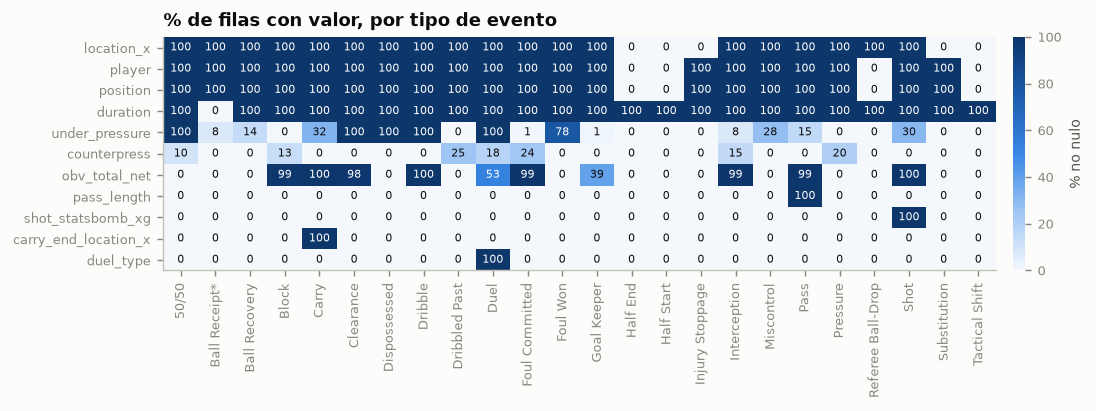
\includegraphics[width=\linewidth]{events_nulos_por_tipo}
\caption{Porcentaje de filas con valor por tipo de evento: cada familia de columnas ``vive'' en un tipo de evento.}\label{fig:nulos}
\end{figure}

\paragraph{Anomalía en la API: \col{passing_ratio}.} La columna \col{team_match_passing_ratio} coincide exactamente con \col{opp_final_third_pass_ratio} en los 221 partidos (media $\approx0.50$), mientras que la precisión real (\col{successful_passes}/\col{passes}) tiene media 0.83. Usarla como precisión de pase habría producido conclusiones falsas (por ejemplo, correlación negativa entre ``precisión'' y posesión). Se sustituye por la métrica calculada.

\paragraph{Otras observaciones.} \col{attendance} tiene 83\% de nulos (no se usa); \col{jersey_number} llega a 303 (dorsales de fuerzas básicas, irrelevante); \col{period} 3--5 aparece en 0.1\% de los eventos (tiempos extra y penales de liguilla) y debe tratarse aparte en análisis por minuto. El \textbf{360 es parcial}: registra a los jugadores visibles en la toma de TV (mediana de 14 de 22), por lo que describe bien lo que ocurre cerca del balón pero no la estructura completa del equipo.

% =====================================================================
\section{Análisis univariado: qué contiene cada tabla}\label{sec:univariado}
% =====================================================================
\subsection{Partidos (\col{matches})}
Cada fila es un partido del América con su contexto: fecha, temporada, fase (\col{competition_stage}), rival, estadio, árbitro, entrenadores y marcador. Se derivan \col{is_home}, \col{opponent}, \col{team_manager}, \col{goals_for}, \col{goals_against} y \col{result}.

\begin{table}[H]
\centering
\scriptsize
\caption{Variables categóricas de partidos: número de categorías, moda y top-5 (\%).}
\label{tab:matches_cat}
\resizebox{\ifdim\width>\linewidth\linewidth\else\width\fi}{!}{%
\begin{tabular}{lrlrp{8.3cm}}
\toprule
\textbf{Columna} & \textbf{Cat.} & \textbf{Moda} & \textbf{\% moda} & \textbf{Top-5 (\% de partidos)} \\
\midrule
season & 6 & 2024/2025 & 21.17 & 2024/2025 (21.2\%) | 2023/2024 (20.7\%) | 2022/2023 (18.9\%) | 2021/2022 (18.0\%) | 2025/2026 (17.1\%) \\
team\_manager & 5 & Jardine & 58.11 & Jardine (58.1\%) | Fernando Ortiz (24.8\%) | Solari (12.2\%) | Almada (4.1\%) | Cervantes (0.9\%) \\
result & 3 & W & 53.15 & W (53.2\%) | D (27.9\%) | L (18.9\%) \\
is\_home & 2 & False & 50.45 & False (50.5\%) | True (49.5\%) \\
competition\_stage & 14 & Clausura & 38.29 & Clausura (38.3\%) | Apertura (34.7\%) | Regular Season (7.7\%) | Apertura - Quarter-finals (3.6\%) | Quarter-finals (2.7\%) \\
opponent & 18 & Cruz Azul & 7.66 & Cruz Azul (7.7\%) | Toluca (7.2\%) | Pachuca (7.2\%) | Puebla (6.8\%) | Guadalajara (6.8\%) \\
stadium & 18 & Estadio Azteca & 34.68 & Estadio Azteca (34.7\%) | Estadio Ciudad de los Deportes (17.1\%) | Estadio Olímpico de Universitario (Ciudad de México) (4.1\%) | Estadio Cuauhtémoc (4.1\%) | Estadio Nemesio Díez (3.6\%) \\
referee & 26 & César Arturo Ramos Palazuelos & 11.26 & César Arturo Ramos Palazuelos (11.3\%) | Víctor Alfonso Cáceres Hernández (9.9\%) | Marco Antonio Ortíz Nava (8.6\%) | Luis Enrique Santander Aguirre (8.1\%) | Fernando Guerrero Ramírez (8.1\%) \\
\bottomrule
\end{tabular}}
\end{table}
\begin{table}[H]
\centering
\small
\caption{Variables numéricas de partidos.}
\label{tab:matches_num}
\resizebox{\ifdim\width>\linewidth\linewidth\else\width\fi}{!}{%
\begin{tabular}{lrrrrrrrrrr}
\toprule
\textbf{Columna} & \textbf{n} & \textbf{\% nulos} & \textbf{Mín} & \textbf{Mediana} & \textbf{Media} & \textbf{Máx} & \textbf{Desv.} & \textbf{Moda} & \textbf{\% moda} & \textbf{\% ceros} \\
\midrule
goals\_for & 222 & 0.00 & 0 & 2.00 & 1.75 & 7 & 1.34 & 1 & 29.28 & 17.57 \\
goals\_against & 222 & 0.00 & 0 & 1.00 & 0.97 & 4 & 1.00 & 0 & 39.19 & 39.19 \\
match\_week & 222 & 0.00 & 1 & 11.00 & 11.23 & 25 & 6.66 & 1 & 4.95 & 0.00 \\
attendance & 38 & 82.88 & 12,560 & 26,970 & 29,963 & 58,445 & 10,786 & 42,610 & 5.26 & 0.00 \\
\bottomrule
\end{tabular}}
\end{table}

La localía está balanceada (49.5\% local). Los rivales más frecuentes son Cruz Azul, Toluca y Pachuca (7--8\% cada uno, por los cruces de liguilla). El América anota en mediana 2 goles y recibe 1; el 39\% de los partidos terminan con portería en cero.

\begin{figure}[H]\centering
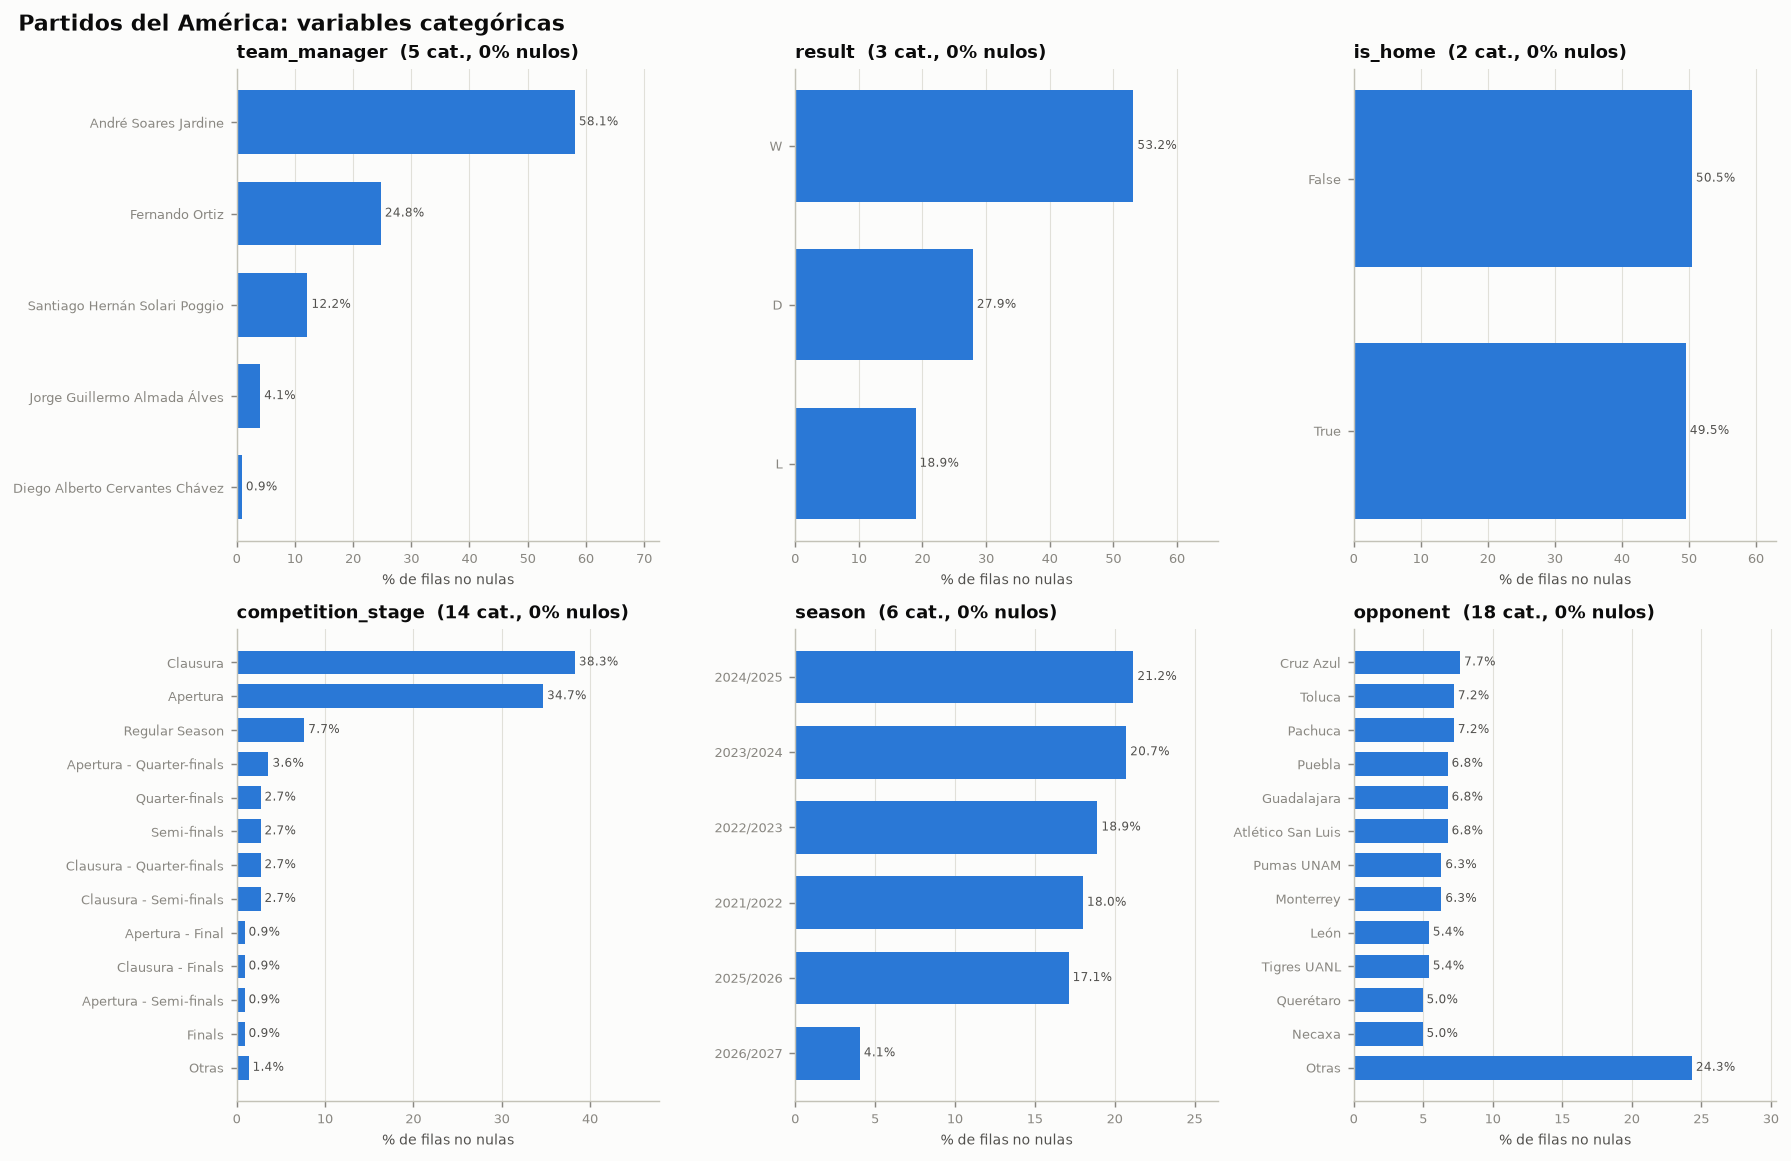
\includegraphics[width=\linewidth]{matches_categoricas}
\caption{Distribución de las variables categóricas de partidos.}
\end{figure}

\begin{table}[H]
\centering
\small
\caption{Resultados del América por entrenador (todas las fases).}
\label{tab:resultado}
\resizebox{\ifdim\width>\linewidth\linewidth\else\width\fi}{!}{%
\begin{tabular}{lrrrrrr}
\toprule
\textbf{Entrenador} & \textbf{\% G} & \textbf{\% E} & \textbf{\% P} & \textbf{Partidos} & \textbf{GF/p} & \textbf{GC/p} \\
\midrule
Jardine & 52.70 & 27.90 & 19.40 & 129 & 1.72 & 0.92 \\
Ortiz & 58.20 & 25.50 & 16.40 & 55 & 2.05 & 1.07 \\
Solari & 40.70 & 33.30 & 25.90 & 27 & 1.15 & 1.00 \\
Almada & 66.70 & 22.20 & 11.10 & 9 & 2.33 & 1.11 \\
Cervantes & 50.00 & 50.00 & 0.00 & 2 & 1.00 & 0.50 \\
\bottomrule
\end{tabular}}
\end{table}

\subsection{Eventos (\col{events})}
Es la tabla principal: 736,829 eventos de ambos equipos (unos 3,300 por partido) y 162 columnas. La Tabla~\ref{tab:events_tipos} resume sus tipos: 60 flags booleanos, 47 numéricas, 36 categóricas y 6 de coordenadas. El significado de cada columna está en el Apéndice~\ref{app:dic}.

\begin{table}[H]
\centering
\small
\caption{Clasificación de las 162 columnas de eventos por tipo analítico.}
\label{tab:events_tipos}
\resizebox{\ifdim\width>\linewidth\linewidth\else\width\fi}{!}{%
\begin{tabular}{lr}
\toprule
\textbf{Tipo analítico} & \textbf{Columnas} \\
\midrule
boolean & 60 \\
numeric & 47 \\
categorical & 36 \\
id & 12 \\
coordinates & 6 \\
json & 4 \\
categorical\_high & 3 \\
datetime & 2 \\
\bottomrule
\end{tabular}}
\end{table}

\subsubsection{Qué tipo de acciones registra}
\begin{table}[H]
\centering
\small
\caption{Frecuencia de los 20 tipos de evento más comunes (ambos equipos).}
\label{tab:events_type}
\resizebox{\ifdim\width>\linewidth\linewidth\else\width\fi}{!}{%
\begin{tabular}{lrrr}
\toprule
\textbf{Tipo de evento} & \textbf{Eventos} & \textbf{\%} & \textbf{\% acum.} \\
\midrule
Pass & 206,473 & 28.02 & 28.02 \\
Ball Receipt* & 189,192 & 25.68 & 53.70 \\
Carry & 166,915 & 22.65 & 76.35 \\
Pressure & 67,072 & 9.10 & 85.45 \\
Ball Recovery & 19,907 & 2.70 & 88.15 \\
Duel & 14,192 & 1.93 & 90.08 \\
Clearance & 8,399 & 1.14 & 91.22 \\
Block & 7,569 & 1.03 & 92.25 \\
Goal Keeper & 6,767 & 0.92 & 93.17 \\
Miscontrol & 5,971 & 0.81 & 93.98 \\
Dribble & 5,806 & 0.79 & 94.77 \\
Foul Committed & 5,771 & 0.78 & 95.55 \\
Shot & 5,675 & 0.77 & 96.32 \\
Foul Won & 5,449 & 0.74 & 97.06 \\
Dispossessed & 5,222 & 0.71 & 97.77 \\
Interception & 3,797 & 0.52 & 98.29 \\
Dribbled Past & 3,403 & 0.46 & 98.75 \\
Substitution & 1,985 & 0.27 & 99.02 \\
Injury Stoppage & 1,379 & 0.19 & 99.21 \\
Half Start & 894 & 0.12 & 99.33 \\
\bottomrule
\end{tabular}}
\end{table}
Pases (28\%), recepciones (26\%) y conducciones (23\%) son tres cuartas partes de los datos: el fútbol se registra como una cadena \emph{pase $\to$ recepción $\to$ conducción}. Las presiones (9\%) son el evento defensivo más frecuente, por encima de recuperaciones, duelos e intercepciones juntos. Los tiros son solo el 0.8\%: \textbf{el gol es un evento raro}, por lo que las métricas de proceso (xG, OBV, progresión) son indispensables para describir el estilo.

\begin{figure}[H]\centering
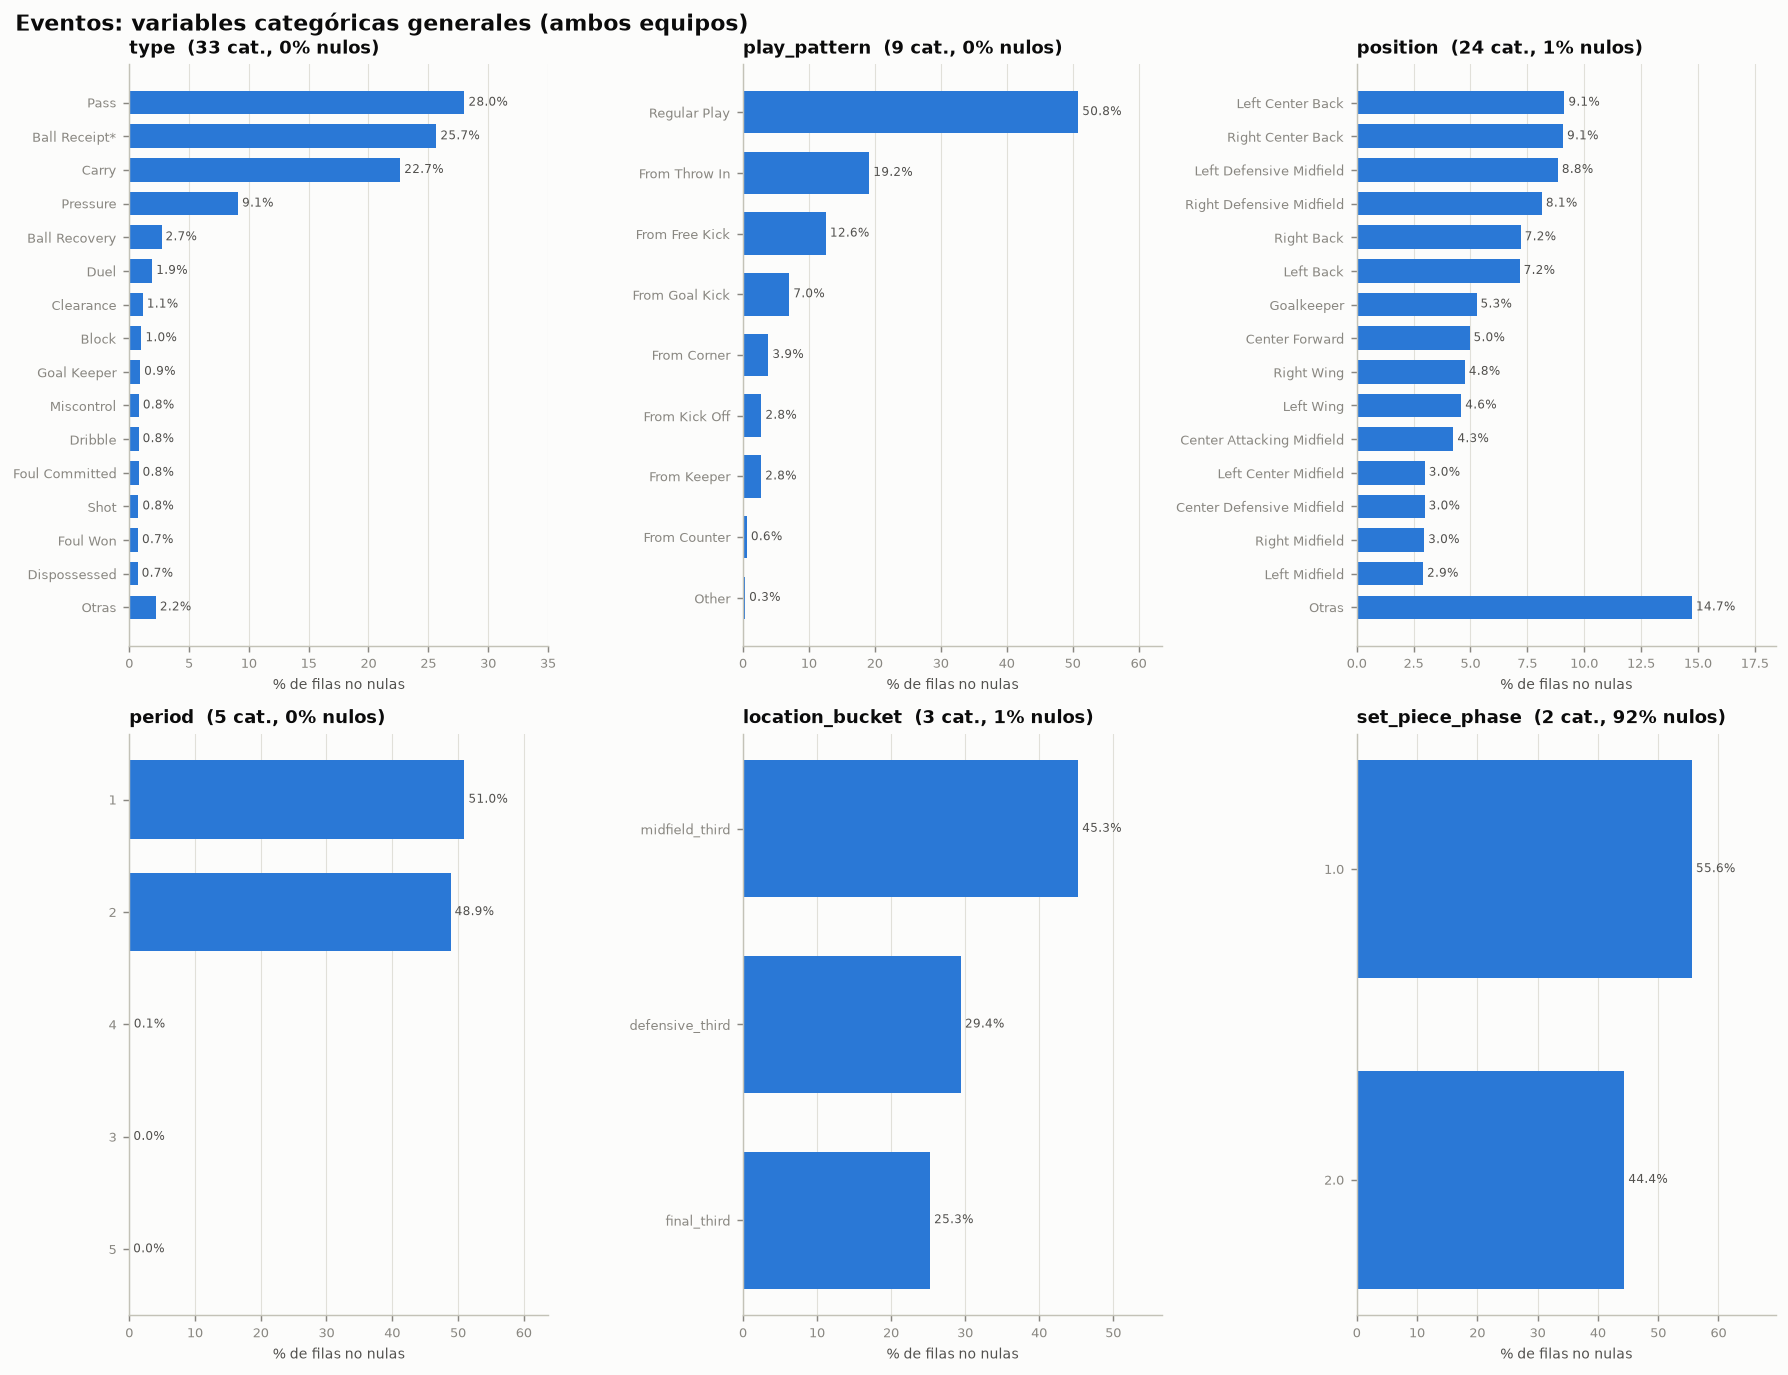
\includegraphics[width=\linewidth]{events_categoricas_generales}
\caption{Variables categóricas generales de eventos (ambos equipos).}\label{fig:events_cat}
\end{figure}
\begin{table}[H]
\centering
\scriptsize
\caption{Variables categóricas generales de eventos.}
\label{tab:events_cat}
\resizebox{\ifdim\width>\linewidth\linewidth\else\width\fi}{!}{%
\begin{tabular}{lrrlrp{7cm}}
\toprule
\textbf{Columna} & \textbf{\% nulos} & \textbf{Cat.} & \textbf{Moda} & \textbf{\% moda} & \textbf{Top-5 (\%)} \\
\midrule
type & 0.00 & 33 & Pass & 28.02 & Pass (28.0\%) | Ball Receipt* (25.7\%) | Carry (22.7\%) | Pressure (9.1\%) | Ball Recovery (2.7\%) \\
play\_pattern & 0.00 & 9 & Regular Play & 50.85 & Regular Play (50.8\%) | From Throw In (19.2\%) | From Free Kick (12.6\%) | From Goal Kick (7.0\%) | From Corner (3.9\%) \\
position & 0.50 & 24 & Left Center Back & 9.13 & Left Center Back (9.1\%) | Right Center Back (9.1\%) | Left Defensive Midfield (8.8\%) | Right Defensive Midfield (8.1\%) | Right Back (7.2\%) \\
period & 0.00 & 5 & 1 & 50.98 & 1 (51.0\%) | 2 (48.9\%) | 4 (0.1\%) | 3 (0.0\%) | 5 (0.0\%) \\
team & 0.00 & 19 & América & 53.40 & América (53.4\%) | Cruz Azul (3.9\%) | Toluca (3.5\%) | Pachuca (3.4\%) | Atlético San Luis (3.3\%) \\
possession\_team & 0.00 & 19 & América & 54.35 & América (54.4\%) | Cruz Azul (3.8\%) | Toluca (3.5\%) | Atlético San Luis (3.3\%) | Pachuca (3.3\%) \\
location\_bucket & 0.97 & 3 & midfield\_third & 45.28 & midfield\_third (45.3\%) | defensive\_third (29.4\%) | final\_third (25.3\%) \\
set\_piece\_phase & 92.14 & 2 & 1.0 & 55.61 & 1.0 (55.6\%) | 2.0 (44.4\%) \\
attacking\_direction & 0.21 & 2 & right\_to\_left & 50.35 & right\_to\_left (50.3\%) | left\_to\_right (49.7\%) \\
\bottomrule
\end{tabular}}
\end{table}

\paragraph{Cómo empiezan las jugadas.} El 51\% de los eventos ocurren en posesiones de juego abierto; el 19\% en posesiones que empezaron con saque de banda, el 13\% con tiro libre, el 7\% con saque de meta y el 4\% con córner. Es decir, \textbf{cerca del 40\% del volumen de juego nace de una reanudación}, y el saque de banda es la más frecuente.

\paragraph{Quién toca el balón.} Las posiciones con más eventos son los centrales (9.1\% cada uno) y los dos mediocampistas defensivos (8.8\% y 8.1\%): el juego pasa por la base de la jugada. \col{location_bucket} confirma que el 45\% de las acciones ocurren en el tercio medio.

\subsubsection{Variables numéricas}
\begin{table}[H]
\centering
\scriptsize
\caption{Variables numéricas de eventos, cada una perfilada sobre el tipo de evento al que aplica.}
\label{tab:events_num}
\resizebox{\ifdim\width>\linewidth\linewidth\else\width\fi}{!}{%
\begin{tabular}{llrrrrrrrrrr}
\toprule
\textbf{Columna} & \textbf{Aplica a} & \textbf{n} & \textbf{\% nulos} & \textbf{Mín} & \textbf{P25} & \textbf{Mediana} & \textbf{Media} & \textbf{P75} & \textbf{Máx} & \textbf{Desv.} & \textbf{Asim.} \\
\midrule
minute & (todas) & 736,829 & 0.000 & 0.000 & 22.000 & 46.000 & 45.829 & 68.000 & 128.000 & 27.501 & 0.076 \\
duration & (todas) & 547,611 & 25.680 & 0.000 & 0.333 & 1.064 & 1.304 & 1.768 & 108.193 & 1.426 & 5.142 \\
location\_x & (todas) & 729,663 & 0.970 & 0.000 & 36.200 & 57.200 & 57.916 & 80.300 & 120.000 & 28.863 & 0.012 \\
location\_y & (todas) & 729,663 & 0.970 & 0.100 & 19.600 & 39.400 & 39.516 & 59.300 & 80.000 & 22.989 & 0.035 \\
obv\_total\_net & (todas) & 418,690 & 43.180 & -1.095 & -0.002 & 0.000 & 0.002 & 0.003 & 1.608 & 0.037 & -0.944 \\
control\_degree & (todas) & 624,520 & 15.240 & 0.000 & 0.676 & 1.000 & 0.789 & 1.000 & 1.000 & 0.354 & -1.352 \\
pass\_length & Pass & 206,473 & 0.000 & 0.000 & 11.500 & 17.800 & 21.761 & 27.320 & 115.800 & 15.128 & 1.712 \\
pass\_angle & Pass & 206,473 & 0.000 & -3.141 & -1.218 & -0.017 & 0.013 & 1.277 & 3.142 & 1.568 & 0.021 \\
pass\_pass\_success\_probability & Pass & 205,504 & 0.470 & 0.020 & 0.719 & 0.943 & 0.813 & 0.983 & 0.999 & 0.245 & -1.346 \\
pass\_xclaim & Pass & 8,630 & 95.820 & 0.000 & 0.001 & 0.011 & 0.041 & 0.045 & 0.729 & 0.074 & 3.108 \\
shot\_statsbomb\_xg & Shot & 5,675 & 0.000 & 0.003 & 0.026 & 0.051 & 0.100 & 0.101 & 0.977 & 0.143 & 3.191 \\
shot\_shot\_execution\_xg & Shot & 5,675 & 0.000 & 0.000 & 0.000 & 0.012 & 0.103 & 0.093 & 0.998 & 0.207 & 2.721 \\
shot\_gk\_save\_difficulty\_xg & Shot & 1,932 & 65.960 & 0.001 & 0.046 & 0.167 & 0.301 & 0.498 & 0.999 & 0.310 & 0.947 \\
duel\_duel\_win\_probability & Duel & 6,521 & 54.050 & 0.066 & 0.367 & 0.462 & 0.464 & 0.557 & 0.946 & 0.134 & 0.061 \\
clearance\_duel\_win\_probability & Clearance & 1,779 & 78.820 & 0.182 & 0.483 & 0.565 & 0.564 & 0.645 & 0.895 & 0.120 & -0.140 \\
\bottomrule
\end{tabular}}
\end{table}

\begin{figure}[H]\centering
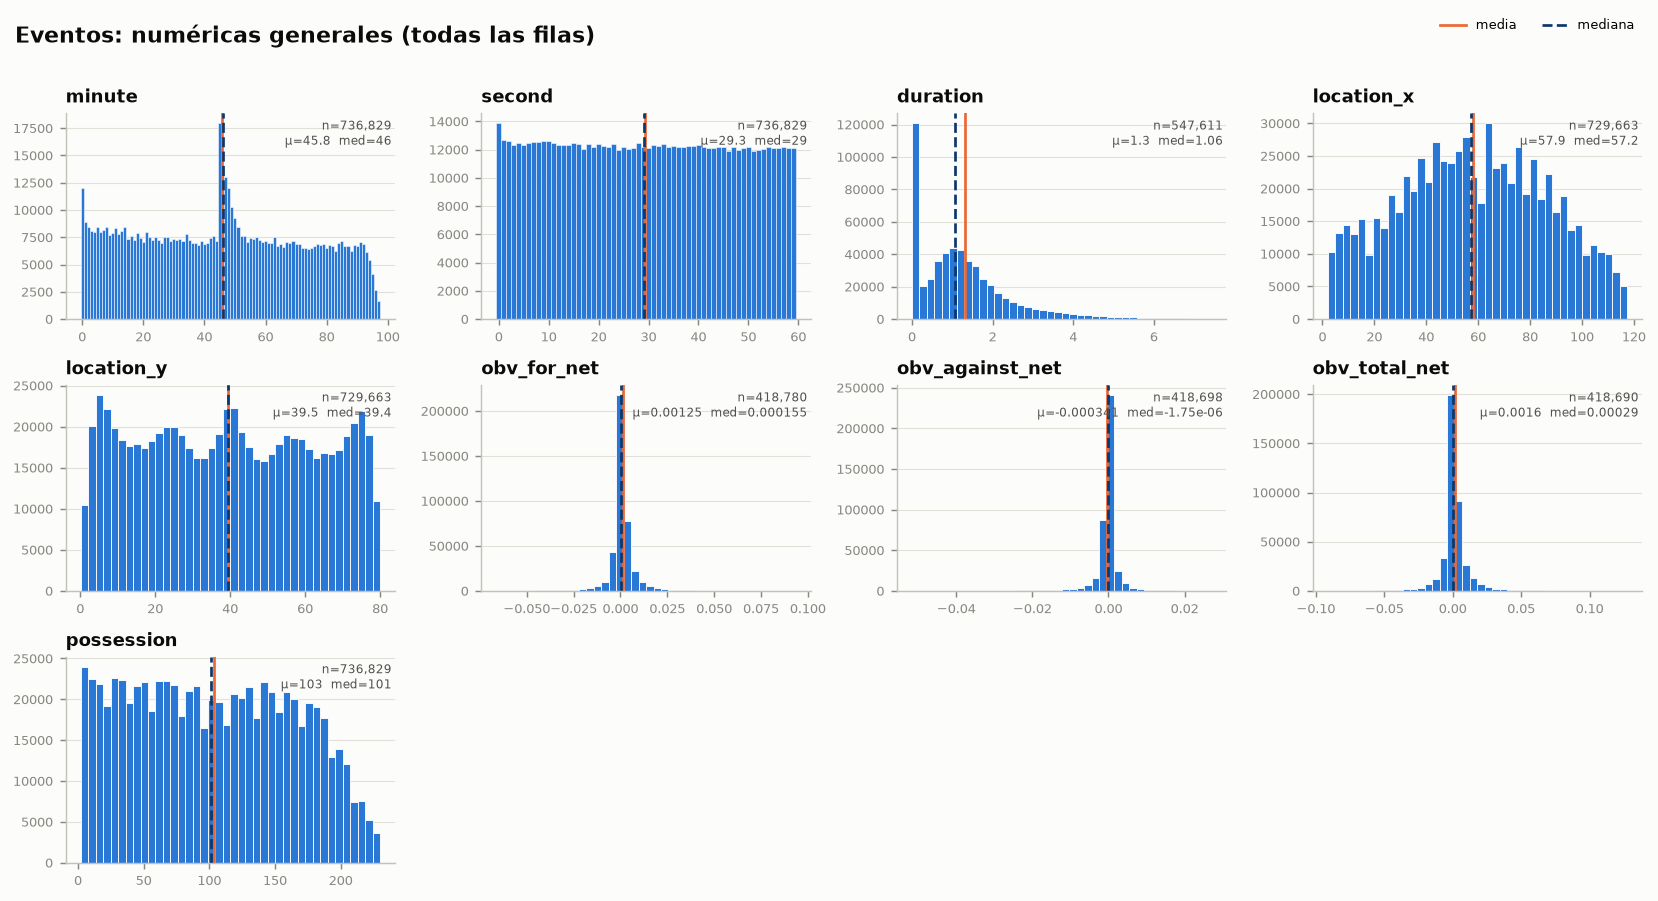
\includegraphics[width=\linewidth]{events_numericas_generales}
\caption{Numéricas generales. El pico en el minuto 45 se debe a que el segundo tiempo arranca en 45, que se suma al tiempo añadido del primero; \col{duration} tiene un pico en 0 (acciones instantáneas); OBV está muy concentrado alrededor de 0 con colas largas.}
\end{figure}

\begin{itemize}
  \item \textbf{Espacio}: \col{location_x} tiene mediana 57 (mitad de la cancha) y $y$ tiene dos picos junto a las bandas (saques de banda y juego por fuera).
  \item \textbf{OBV}: la mediana es prácticamente 0 y las colas son largas. Casi todas las acciones valen poco y unas pocas (pases clave, tiros, pérdidas en zona propia) concentran el valor.
  \item \textbf{Posesión}: el número de posesión llega hasta unas 230 por partido.
\end{itemize}

\begin{figure}[H]\centering
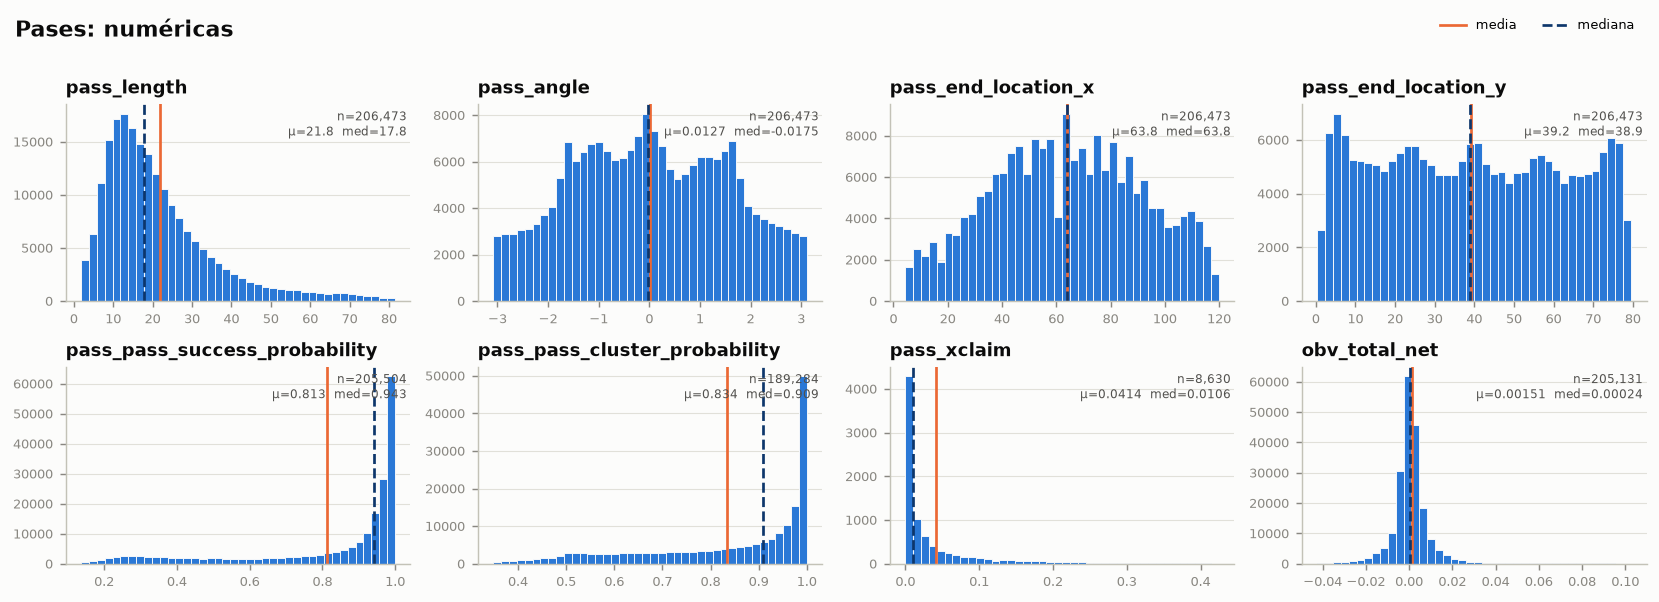
\includegraphics[width=\linewidth]{events_pases_numericas}
\caption{Pases: longitud (mediana 17.8 yardas, asimetría a la derecha), ángulo (bimodal: pases hacia adelante y laterales), probabilidad de éxito (mediana 0.94).}
\end{figure}

\begin{figure}[H]\centering
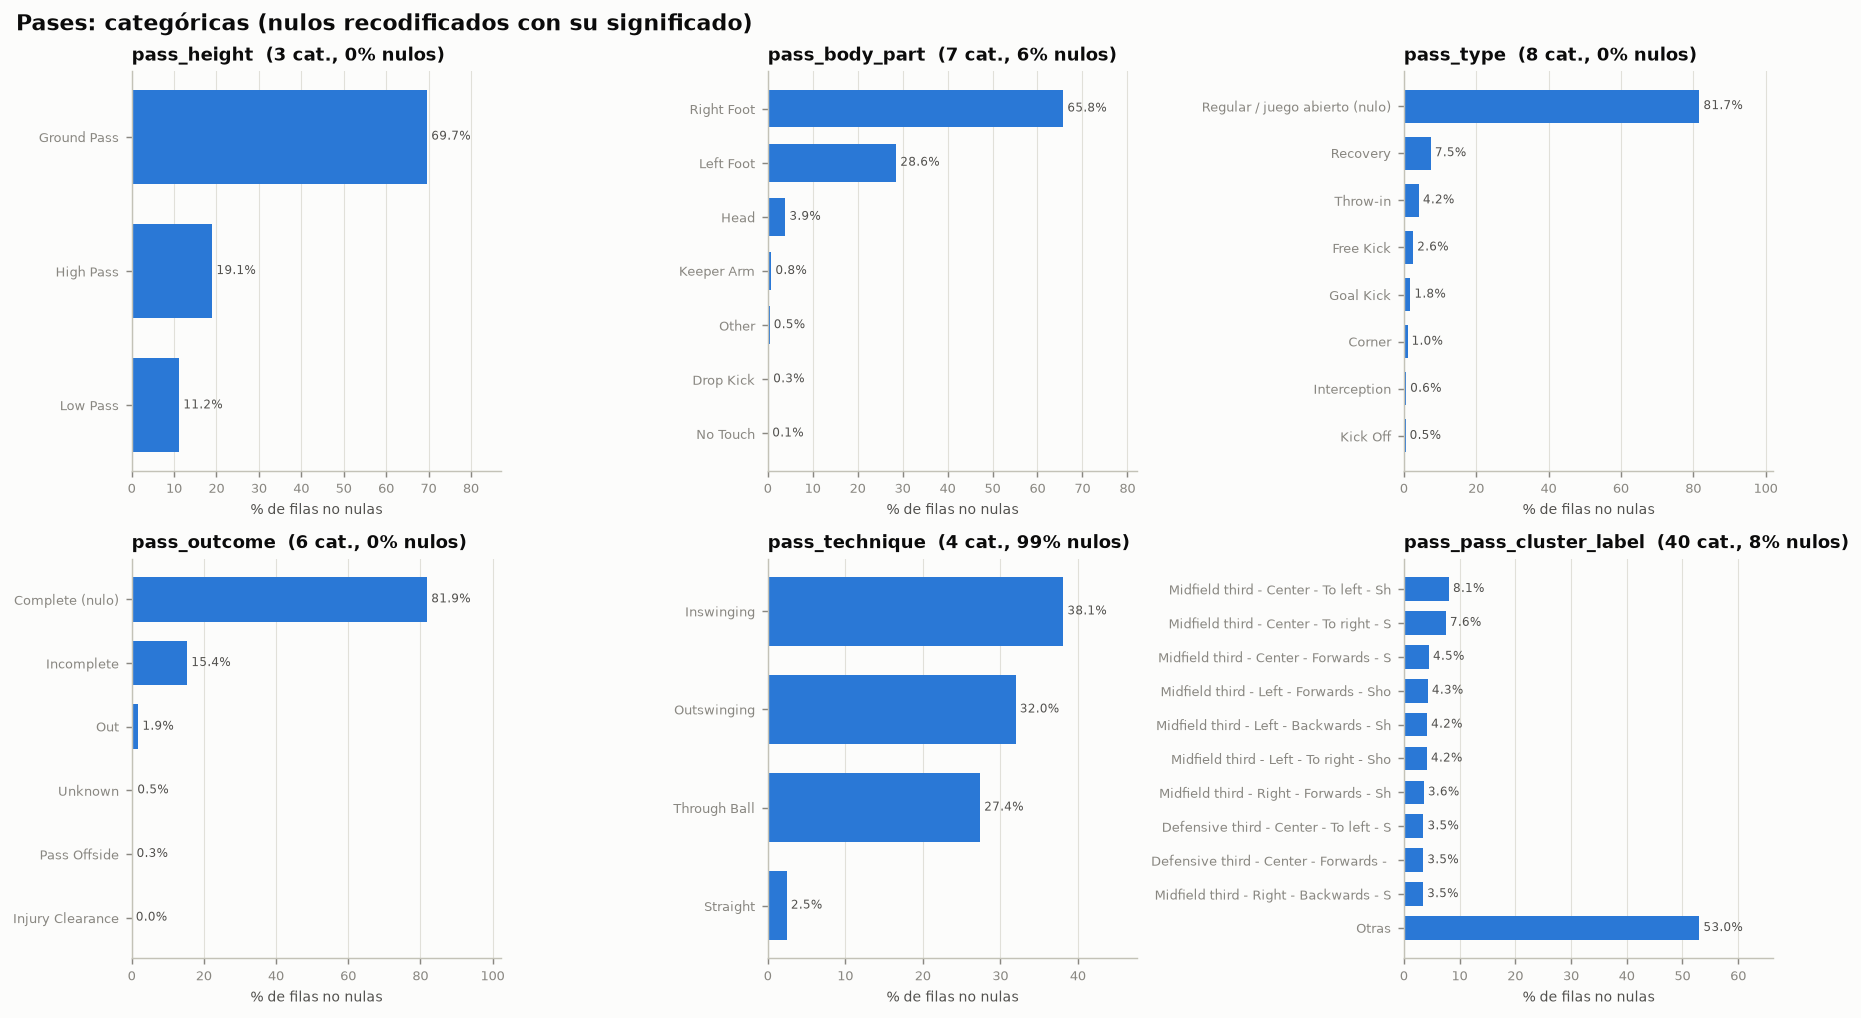
\includegraphics[width=\linewidth]{events_pases_categoricas}
\caption{Pases: 70\% por el suelo, 66\% con pierna derecha. En \col{pass_type} el nulo significa ``pase regular''; en \col{pass_outcome}, ``pase completo'' (alrededor del 82\%).}
\end{figure}

\begin{figure}[H]\centering
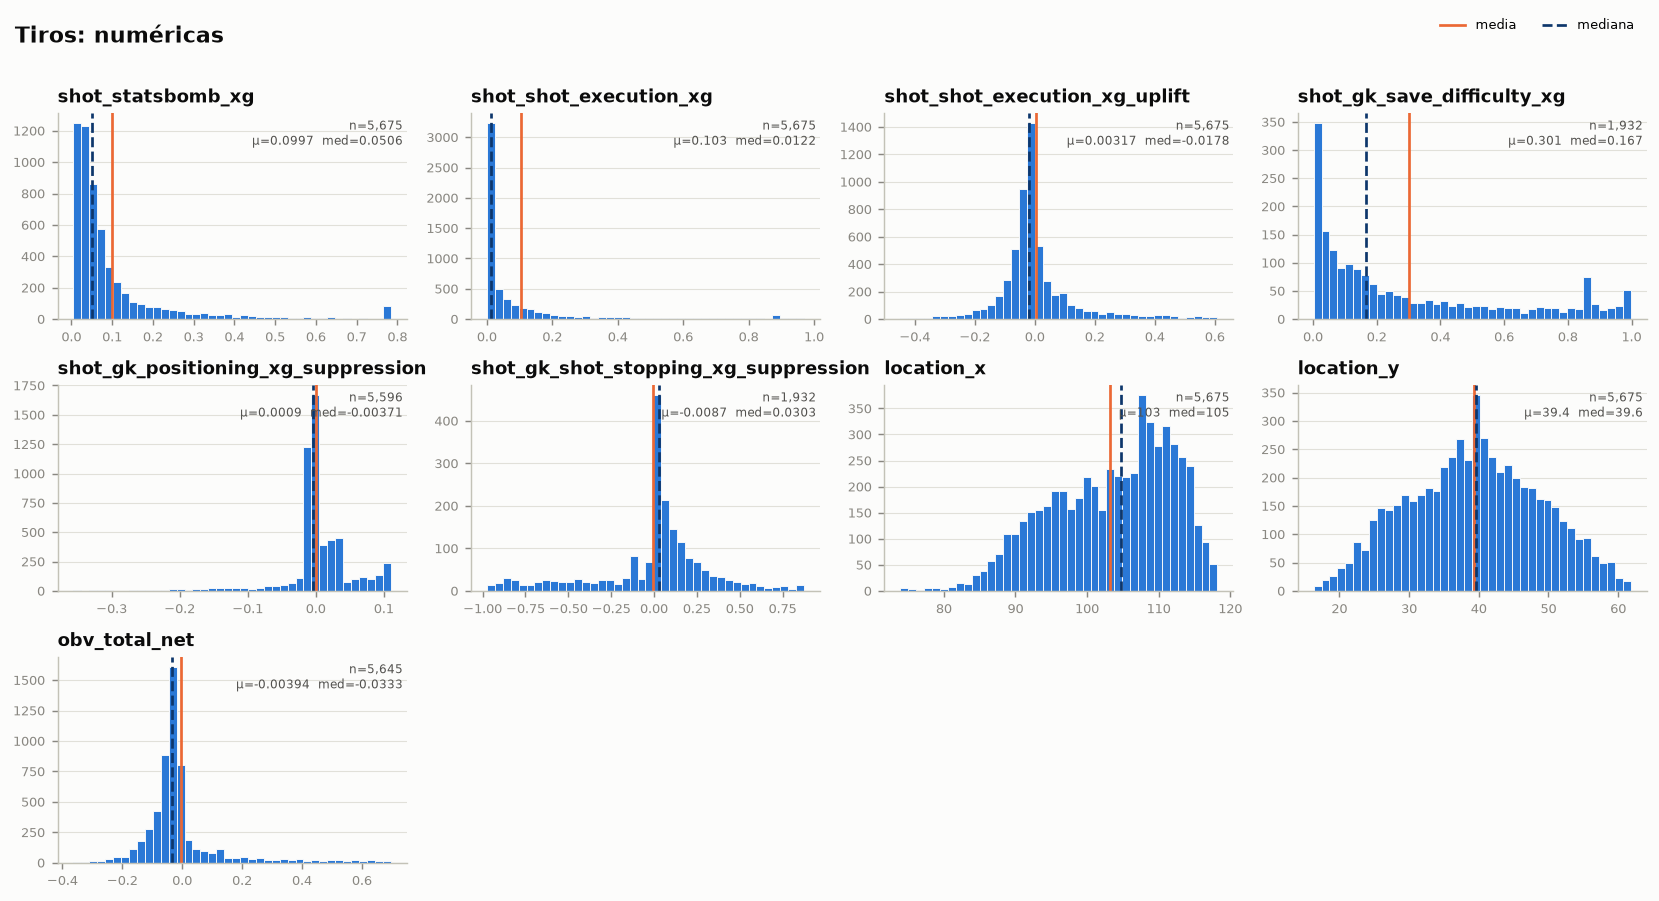
\includegraphics[width=\linewidth]{events_tiros_numericas}
\caption{Tiros: xG mediano 0.05, con un pico cerca de 0.78 que corresponde a los penales (1.4\% de los tiros). La mayoría se remata entre $x=95$ y $x=115$.}
\end{figure}

\begin{figure}[H]\centering
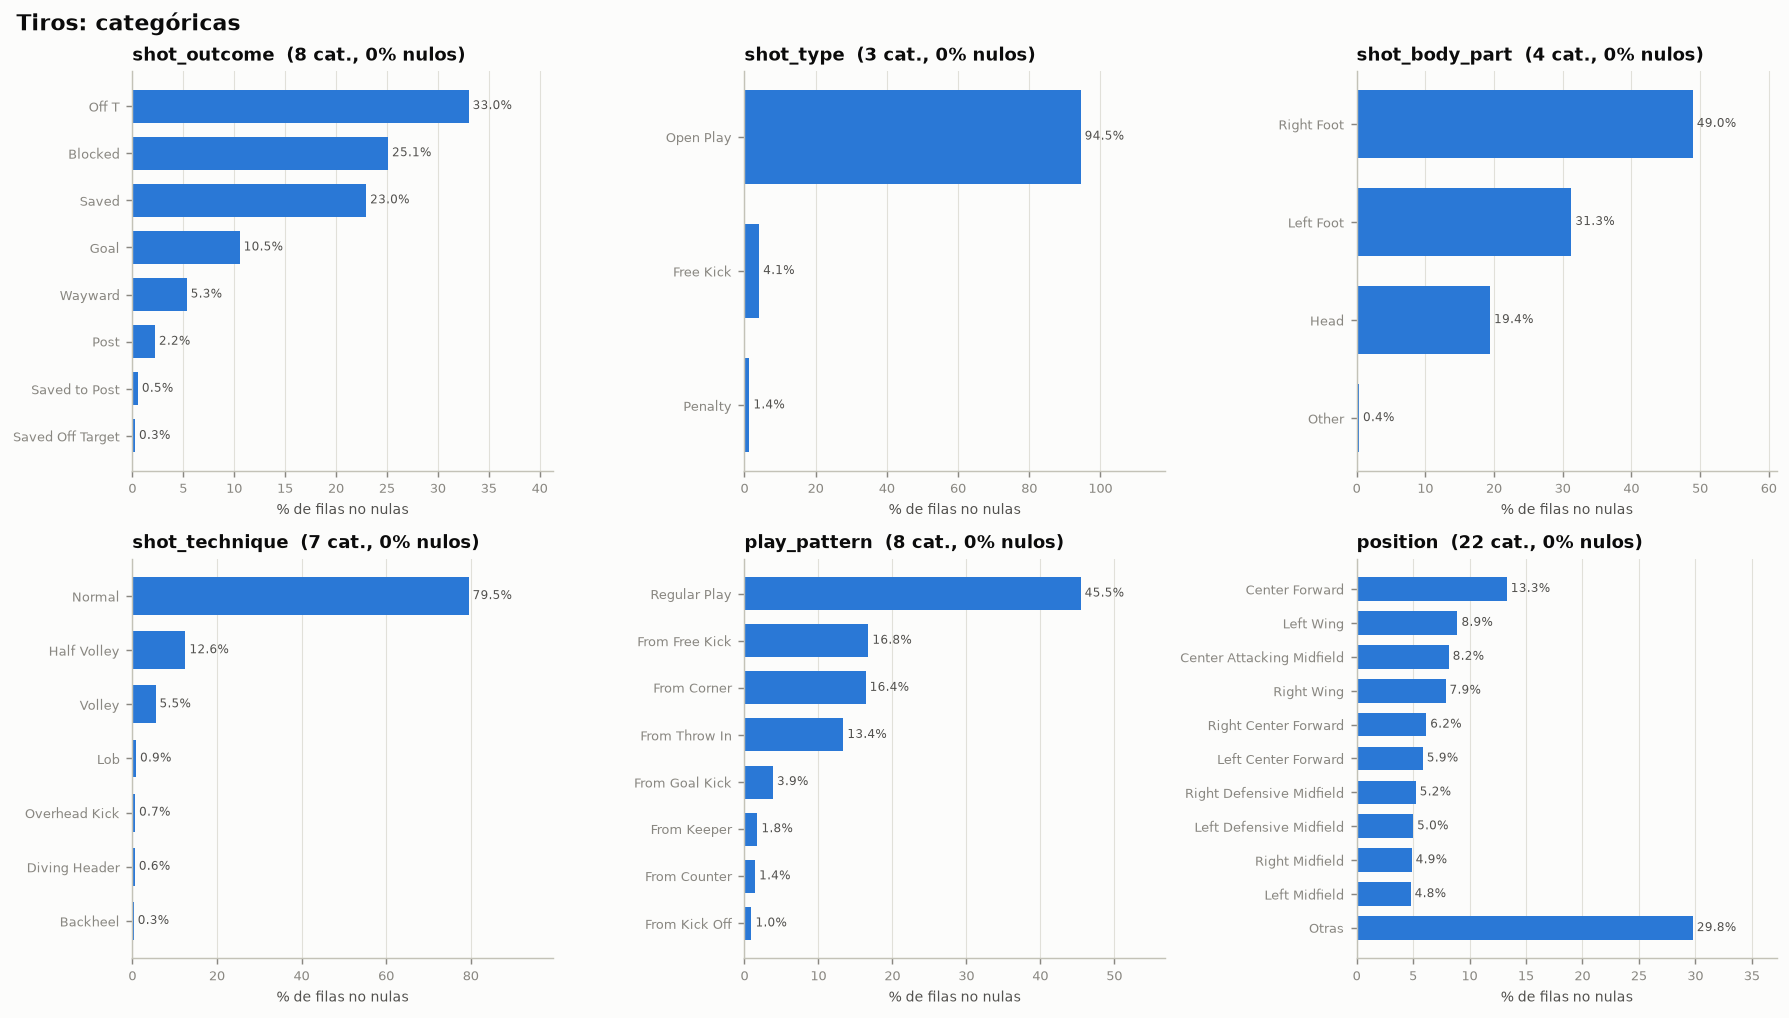
\includegraphics[width=\linewidth]{events_tiros_categoricas}
\caption{Tiros: el 10.5\% termina en gol, el 33\% va desviado y el 25\% es bloqueado. El 45.5\% nace de juego abierto, y el resto de tiros libres (16.8\%), córners (16.4\%) y saques de banda (13.4\%). El delantero centro es la posición que más remata (13.3\%).}
\end{figure}

\begin{figure}[H]\centering
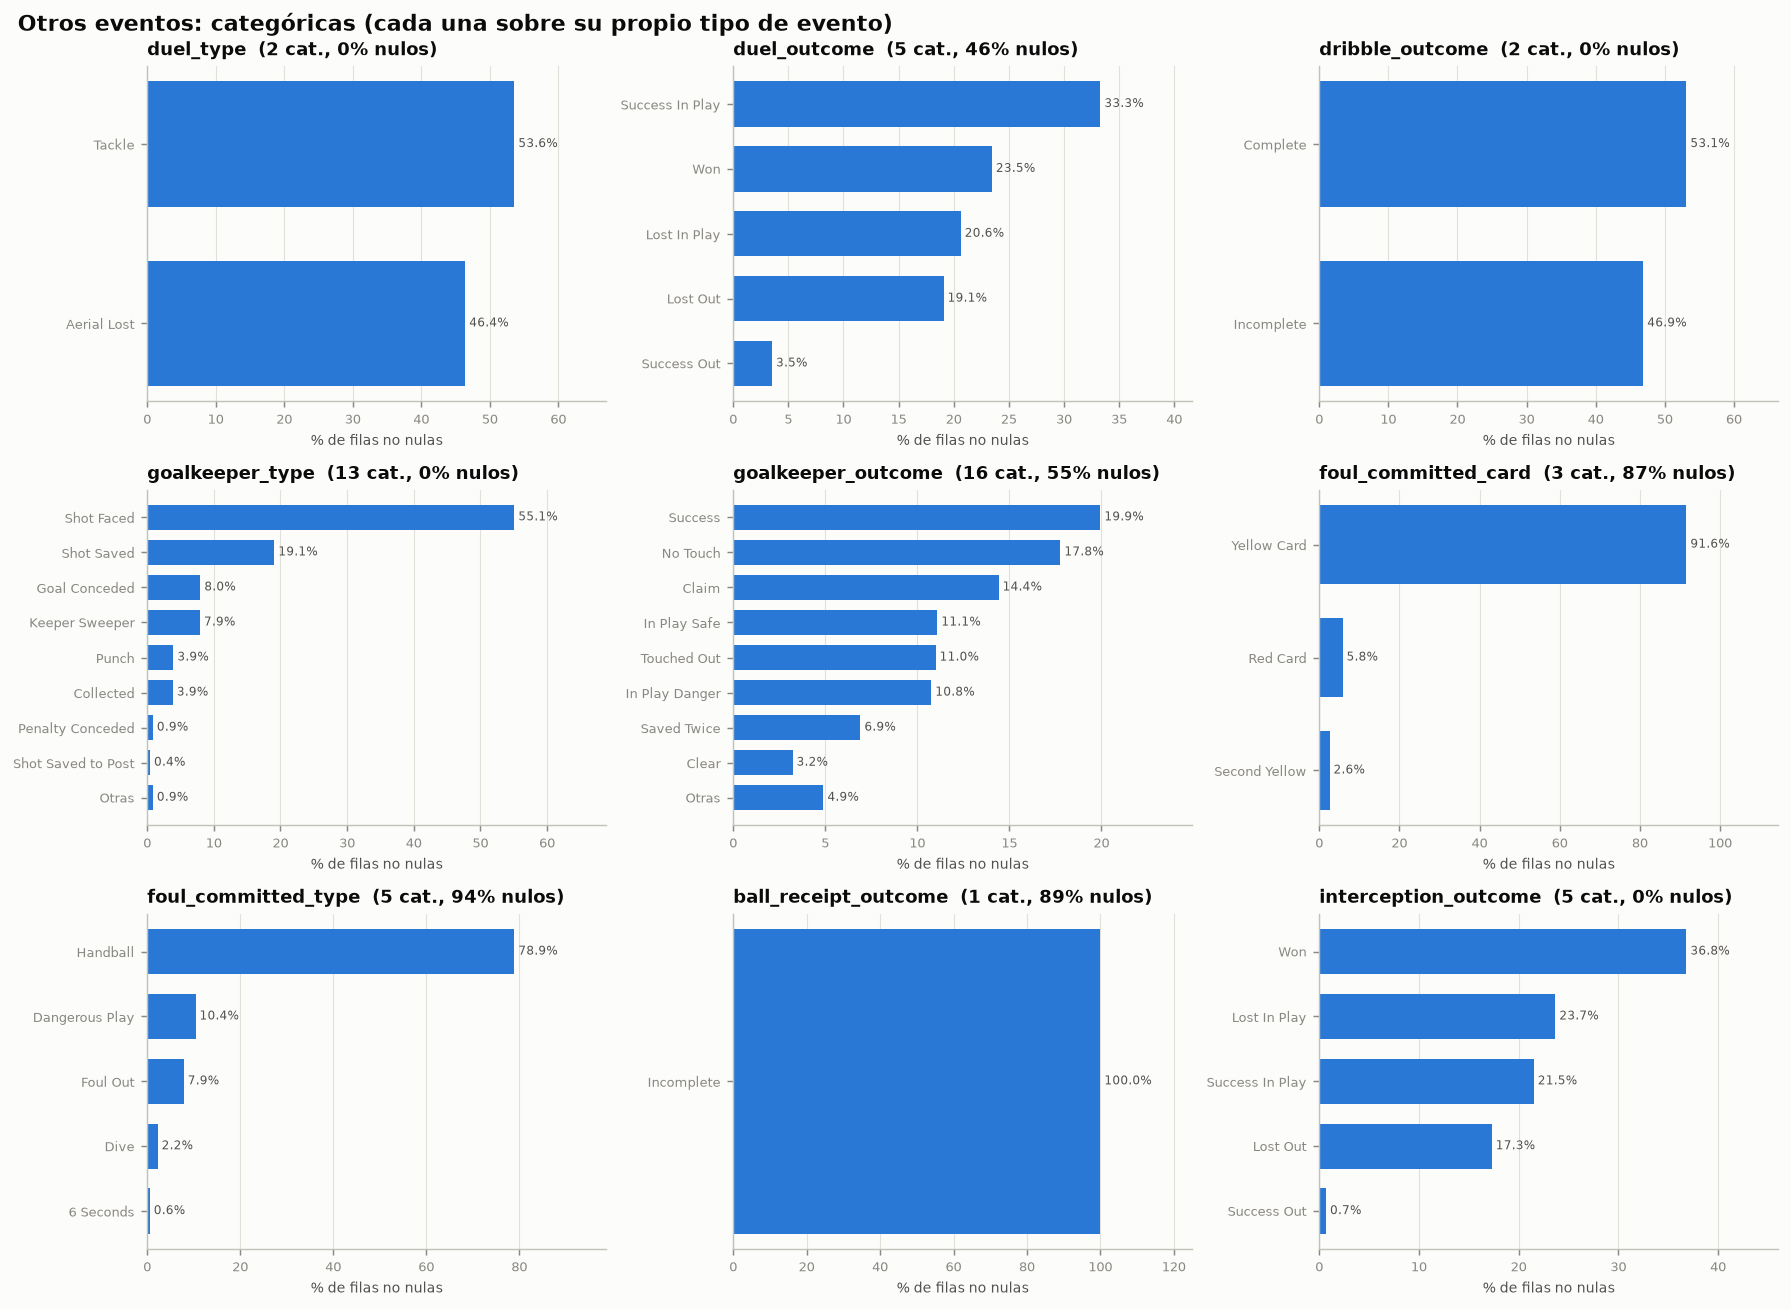
\includegraphics[width=\linewidth]{events_otros_categoricas}
\caption{Otros eventos, cada uno perfilado sobre su propio tipo: duelos, regates, acciones del portero, faltas, recepciones e intercepciones.}
\end{figure}

\begin{figure}[H]\centering
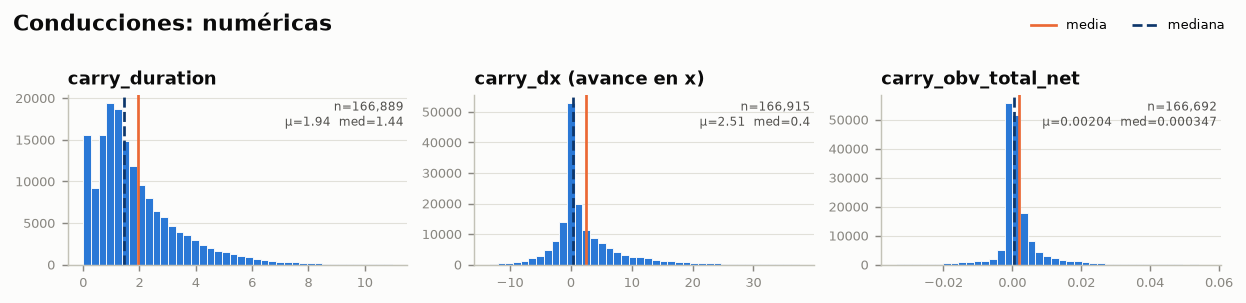
\includegraphics[width=0.85\linewidth]{events_conducciones_numericas}
\caption{Conducciones: la mayoría son cortas y con avance pequeño en $x$; la conducción funciona como enlace entre pases.}
\end{figure}

\subsubsection{Flags booleanos}
{\scriptsize
\begin{longtable}{llrrr}
\caption{Flags booleanos (\% de filas con \texttt{True} dentro del tipo de evento; NaN = False). Se muestran los que superan 1\%.}\label{tab:events_bool}\\
\toprule
\textbf{Flag} & \textbf{Aplica a} & \textbf{Filas} & \textbf{True} & \textbf{\% True} \\
\midrule
\endfirsthead
\toprule
\textbf{Flag} & \textbf{Aplica a} & \textbf{Filas} & \textbf{True} & \textbf{\% True} \\
\midrule
\endhead
\bottomrule
\endfoot
is\_controlled\_possession & (todas) & 736,829 & 524,248 & 71.15 \\
is\_home & (todas) & 736,829 & 367,612 & 49.89 \\
is\_transition & (todas) & 736,829 & 197,314 & 26.78 \\
under\_pressure & (todas) & 736,829 & 144,843 & 19.66 \\
counterpress & (todas) & 736,829 & 20,014 & 2.72 \\
off\_camera & (todas) & 736,829 & 10,308 & 1.40 \\
out & (todas) & 736,829 & 10,066 & 1.37 \\
ball\_recovery\_recovery\_failure & Ball Recovery & 19,907 & 1,426 & 7.16 \\
block\_deflection & Block & 7,569 & 201 & 2.66 \\
block\_offensive & Block & 7,569 & 155 & 2.05 \\
clearance\_head & Clearance & 8,399 & 4,725 & 56.26 \\
clearance\_right\_foot & Clearance & 8,399 & 2,181 & 25.97 \\
clearance\_aerial\_won & Clearance & 8,399 & 1,798 & 21.41 \\
clearance\_left\_foot & Clearance & 8,399 & 1,434 & 17.07 \\
dribble\_overrun & Dribble & 5,806 & 393 & 6.77 \\
dribble\_nutmeg & Dribble & 5,806 & 362 & 6.23 \\
foul\_committed\_advantage & Foul Committed & 5,771 & 663 & 11.49 \\
foul\_committed\_offensive & Foul Committed & 5,771 & 218 & 3.78 \\
foul\_committed\_penalty & Foul Committed & 5,771 & 69 & 1.20 \\
foul\_won\_defensive & Foul Won & 5,449 & 1,400 & 25.69 \\
foul\_won\_advantage & Foul Won & 5,449 & 653 & 11.98 \\
injury\_stoppage\_in\_chain & Injury Stoppage & 1,379 & 285 & 20.67 \\
miscontrol\_aerial\_won & Miscontrol & 5,971 & 218 & 3.65 \\
pass\_switch & Pass & 206,473 & 6,768 & 3.28 \\
pass\_cross & Pass & 206,473 & 5,155 & 2.50 \\
pass\_aerial\_won & Pass & 206,473 & 3,972 & 1.92 \\
pass\_shot\_assist & Pass & 206,473 & 3,805 & 1.84 \\
shot\_first\_time & Shot & 5,675 & 1,875 & 33.04 \\
shot\_aerial\_won & Shot & 5,675 & 600 & 10.57 \\
shot\_one\_on\_one & Shot & 5,675 & 271 & 4.78 \\
shot\_follows\_dribble & Shot & 5,675 & 244 & 4.30 \\
shot\_deflected & Shot & 5,675 & 84 & 1.48 \\
\end{longtable}
}
Dos flags son especialmente relevantes para el reto. \col{under_pressure} está en el 19.7\% de todos los eventos, y en pases y conducciones permite medir cómo juega el equipo cuando lo presionan. \col{counterpress} aparece en el 2.7\% de los eventos y mide la reacción tras pérdida. StatsBomb además marca \col{is_transition} (26.8\% de eventos) e \col{is_controlled_possession} (71.2\%), que dan una base directa para separar el juego de transición del juego posicional.

\subsubsection{Dónde ocurren las acciones}
\begin{figure}[H]\centering
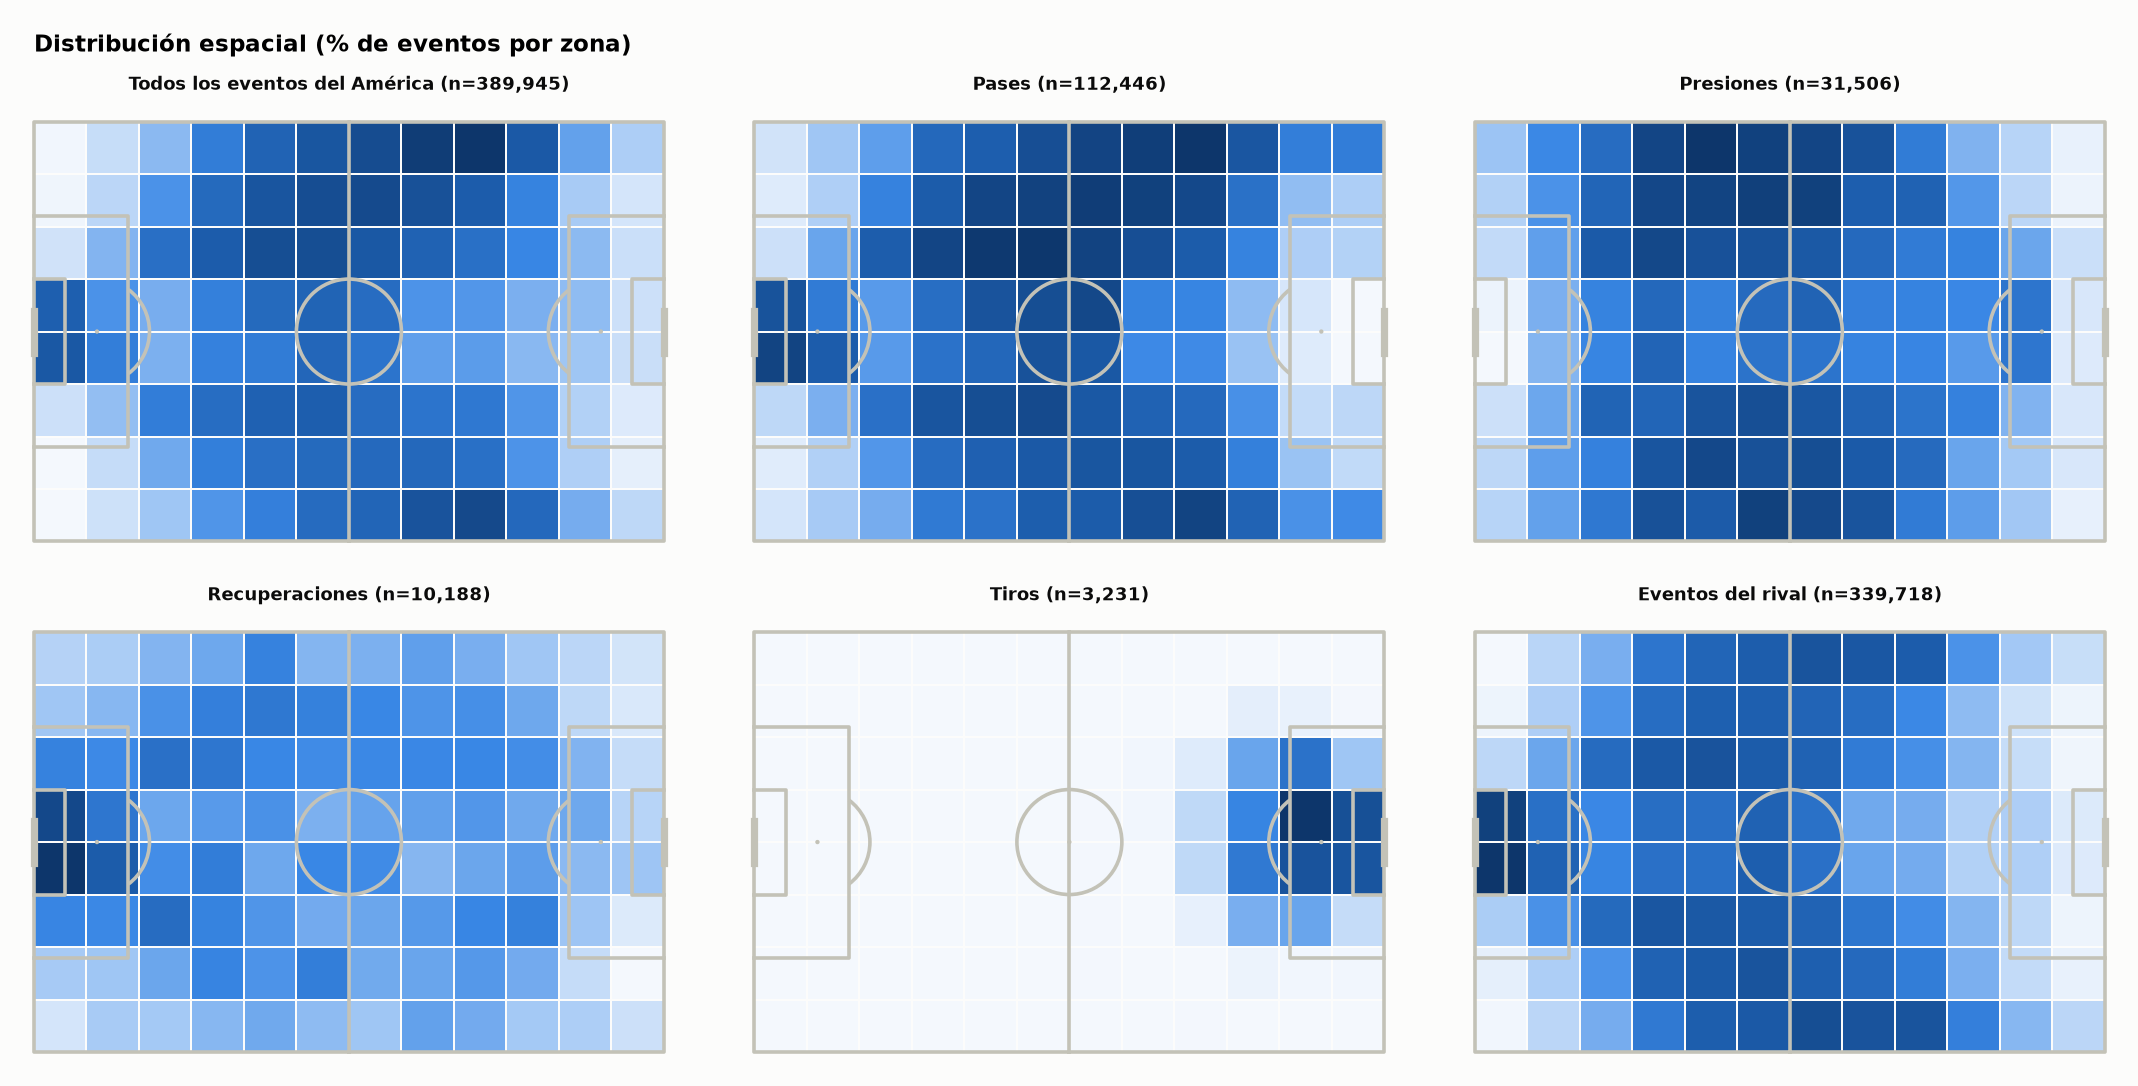
\includegraphics[width=\linewidth]{events_mapas_calor}
\caption{Distribución espacial (\% de eventos por zona). El América acumula sus pases en el tercio medio y por las bandas, presiona sobre todo en el medio campo y en la franja central, recupera en toda la cancha con un foco en su propia área y remata casi siempre desde dentro del área.}\label{fig:mapas}
\end{figure}

\subsubsection{Posesiones}
\begin{table}[H]
\centering
\small
\caption{Perfil de las 47,033 posesiones (ambos equipos).}
\label{tab:posesiones}
\resizebox{\ifdim\width>\linewidth\linewidth\else\width\fi}{!}{%
\begin{tabular}{lrrrrrrrrrr}
\toprule
\textbf{Variable} & \textbf{n} & \textbf{Mín} & \textbf{P25} & \textbf{Mediana} & \textbf{Media} & \textbf{P75} & \textbf{P95} & \textbf{Máx} & \textbf{\% ceros} & \textbf{Asim.} \\
\midrule
eventos & 47,033 & 1.00 & 5.00 & 10.00 & 15.67 & 20.00 & 47.00 & 212.00 & 0.00 & 2.46 \\
pases & 47,033 & 0.00 & 1.00 & 3.00 & 4.39 & 6.00 & 14.00 & 64.00 & 7.59 & 2.51 \\
x inicial & 46,371 & 0.10 & 19.80 & 44.10 & 48.28 & 69.70 & 114.00 & 120.00 & 0.00 & 0.52 \\
x máxima & 46,371 & 1.30 & 77.70 & 94.20 & 90.13 & 108.10 & 118.70 & 120.00 & 0.00 & -1.28 \\
duración (s) & 47,033 & 0.00 & 4.22 & 9.57 & 15.19 & 20.40 & 48.26 & 184.96 & 2.08 & 2.32 \\
xG & 47,033 & 0.00 & 0.00 & 0.00 & 0.01 & 0.00 & 0.06 & 1.52 & 88.84 & 9.46 \\
\bottomrule
\end{tabular}}
\end{table}
\begin{figure}[H]\centering
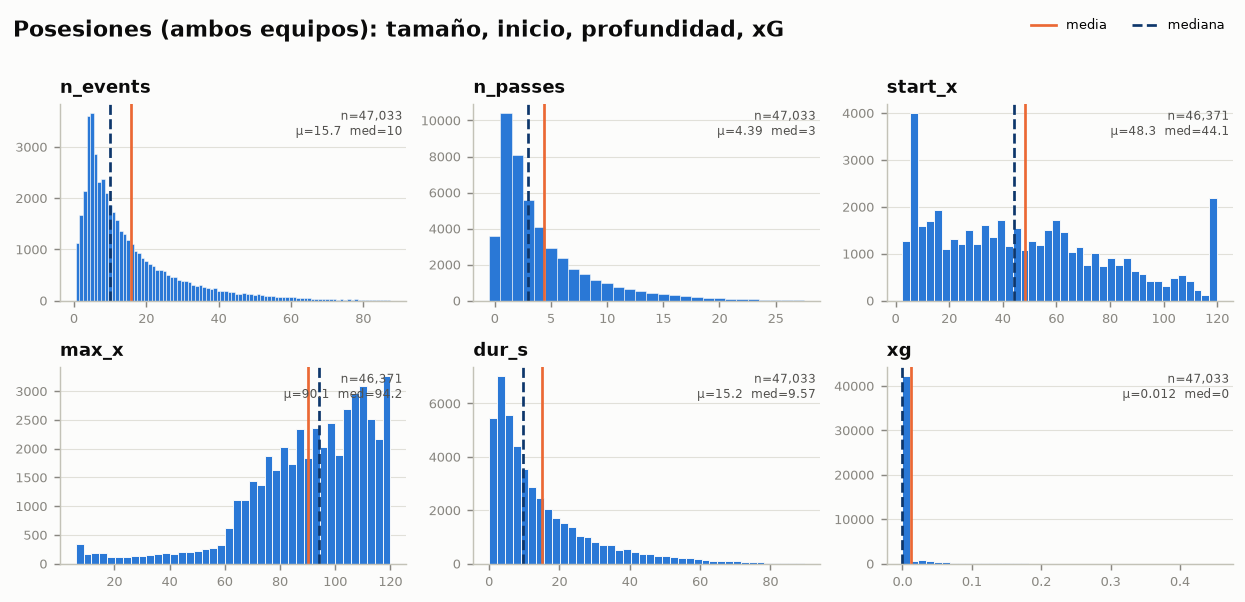
\includegraphics[width=0.9\linewidth]{posesiones_numericas}
\caption{Posesiones de ambos equipos. La mediana es de 3 pases; la $x$ inicial tiene picos en la propia área (saques de meta) y en $x=120$ (saques de esquina). El xG es 0 en el 89\% de las posesiones.}
\end{figure}
Hay unas 212 posesiones por partido y solo el \textbf{11\% termina en tiro}. La mayoría son cortas: la mediana es de 10 eventos y 9.6 segundos. Esto confirma que la unidad de análisis de estilo tiene que ser la posesión o la secuencia, y no el evento suelto.

\subsection{Métricas por equipo y partido (\col{team_match_stats})}
Son 216 columnas: 199 métricas numéricas calculadas por StatsBomb para cada equipo en cada partido, organizadas en familias (Apéndice, Tabla~\ref{tab:dic_familias}). Aquí se perfilan las 221 filas del América. Las métricas del rival aparecen con el sufijo \col{_conceded}.

\begin{table}[H]
\centering
\scriptsize
\caption{Métricas clave del América por partido (221 partidos).}
\label{tab:team_num}
\resizebox{\ifdim\width>\linewidth\linewidth\else\width\fi}{!}{%
\begin{tabular}{lrrrrrrrr}
\toprule
\textbf{Métrica} & \textbf{Mín} & \textbf{P25} & \textbf{Mediana} & \textbf{Media} & \textbf{P75} & \textbf{Máx} & \textbf{Desv.} & \textbf{Asim.} \\
\midrule
np\_xg & 0.09 & 0.89 & 1.24 & 1.37 & 1.76 & 4.19 & 0.74 & 1.14 \\
np\_xg\_conceded & 0.00 & 0.49 & 0.78 & 0.86 & 1.13 & 2.99 & 0.50 & 1.12 \\
np\_xgd & -1.83 & -0.11 & 0.44 & 0.51 & 1.02 & 3.44 & 0.93 & 0.43 \\
possession & 0.28 & 0.48 & 0.55 & 0.54 & 0.61 & 0.75 & 0.09 & -0.37 \\
ppda & 2.88 & 7.97 & 10.54 & 11.89 & 13.82 & 47.25 & 6.24 & 2.42 \\
defensive\_distance & 32.41 & 41.75 & 44.98 & 45.20 & 48.50 & 61.76 & 5.03 & 0.21 \\
directness & 0.39 & 0.83 & 0.88 & 0.87 & 0.92 & 0.99 & 0.08 & -2.25 \\
pace\_towards\_goal & 0.56 & 2.10 & 2.54 & 2.63 & 3.16 & 6.00 & 0.80 & 0.67 \\
gk\_long\_pass\_ratio & 0.00 & 0.38 & 0.50 & 0.50 & 0.60 & 1.00 & 0.17 & 0.42 \\
pass\_completion & 0.59 & 0.81 & 0.84 & 0.83 & 0.86 & 0.92 & 0.05 & -1.20 \\
deep\_progressions & 19.00 & 40.00 & 48.00 & 50.48 & 60.00 & 91.00 & 15.74 & 0.45 \\
deep\_completions & 0.00 & 2.00 & 3.00 & 4.19 & 6.00 & 16.00 & 2.85 & 0.86 \\
box\_cross\_ratio & 0.00 & 0.26 & 0.33 & 0.33 & 0.39 & 0.65 & 0.11 & 0.20 \\
passes\_inside\_box & 0.00 & 1.00 & 2.00 & 2.80 & 4.00 & 13.00 & 2.23 & 0.92 \\
counter\_attacking\_shots & 0.00 & 0.00 & 1.00 & 1.14 & 2.00 & 5.00 & 1.16 & 1.10 \\
high\_press\_shots & 0.00 & 2.00 & 3.00 & 3.45 & 5.00 & 12.00 & 2.19 & 0.71 \\
pressures & 70.00 & 115.00 & 138.00 & 141.89 & 164.00 & 276.00 & 39.07 & 0.81 \\
counterpressures & 10.00 & 22.00 & 27.00 & 28.53 & 35.00 & 57.00 & 8.79 & 0.40 \\
fhalf\_pressures\_ratio & 0.23 & 0.39 & 0.47 & 0.46 & 0.53 & 0.72 & 0.09 & 0.00 \\
pressure\_regains & 9.00 & 24.00 & 32.00 & 33.87 & 41.00 & 82.00 & 13.62 & 0.83 \\
aggression & 0.09 & 0.16 & 0.19 & 0.20 & 0.24 & 0.33 & 0.05 & 0.25 \\
obv & -2.10 & 1.16 & 1.94 & 1.92 & 2.66 & 5.71 & 1.27 & 0.17 \\
obv\_conceded & -2.09 & 0.51 & 1.24 & 1.24 & 2.02 & 4.60 & 1.14 & 0.01 \\
transition\_possession\_rate & 0.10 & 0.17 & 0.19 & 0.19 & 0.22 & 0.28 & 0.03 & 0.03 \\
transition\_xg & 0.00 & 0.10 & 0.23 & 0.36 & 0.51 & 2.03 & 0.36 & 1.68 \\
sp\_xg & 0.00 & 0.12 & 0.24 & 0.30 & 0.42 & 1.21 & 0.26 & 1.32 \\
sp\_xg\_conceded & 0.00 & 0.06 & 0.16 & 0.24 & 0.34 & 1.15 & 0.23 & 1.36 \\
corners & 1.00 & 3.00 & 5.00 & 5.42 & 7.00 & 16.00 & 2.89 & 1.13 \\
xg\_per\_corner & 0.00 & 0.01 & 0.02 & 0.04 & 0.05 & 0.27 & 0.05 & 2.53 \\
gd & -4.00 & 0.00 & 1.00 & 0.76 & 2.00 & 7.00 & 1.69 & 0.42 \\
\bottomrule
\end{tabular}}
\end{table}
\begin{figure}[H]\centering
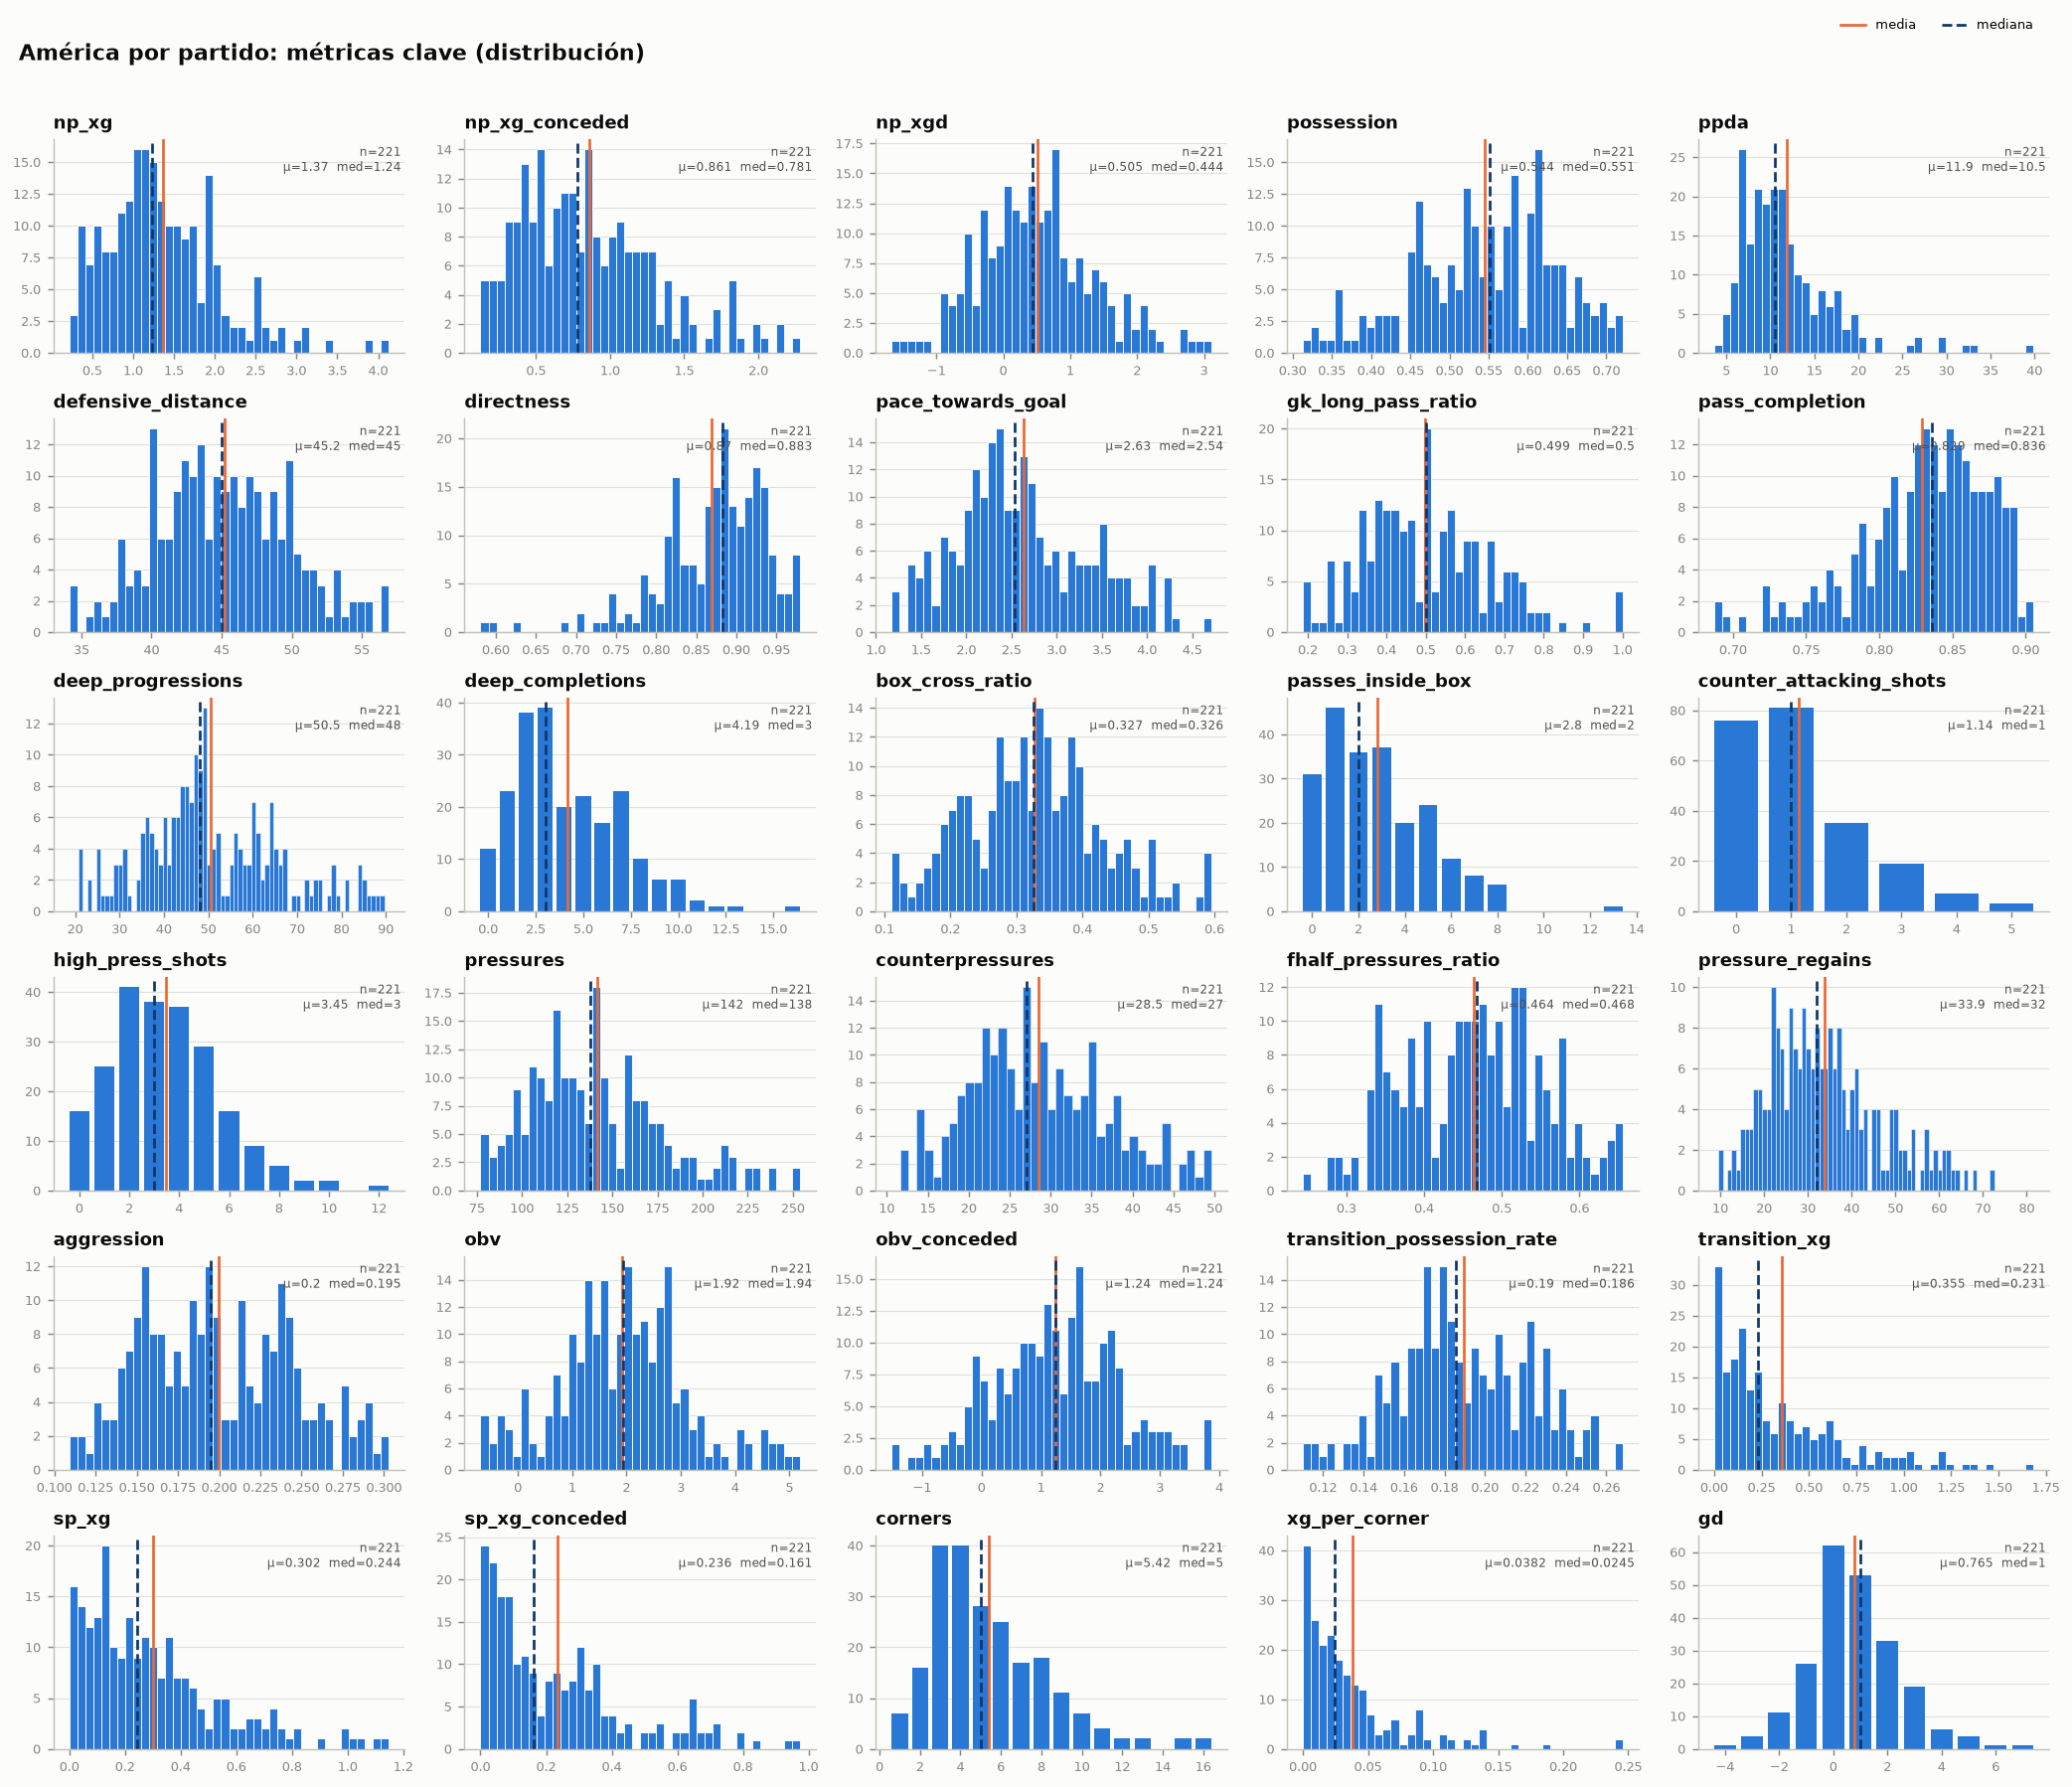
\includegraphics[width=\linewidth]{team_numericas_clave}
\caption{Distribución por partido de las métricas clave del América.}\label{fig:team_num}
\end{figure}
En mediana, el América genera 1.24 de np xG y concede 0.78, con posesión de 0.55 y PPDA de 10.5. El PPDA tiene cola derecha: hay partidos con PPDA mayor a 25, que indican presión muy baja. El xG de balón parado (\col{sp_xg}) y el de transición (\col{transition_xg}) están inflados en ceros, lo que sugiere que su aporte depende del partido.

\subsection{Métricas por jugador y partido (\col{player_match_stats})}
Son 175 métricas por jugador (3,458 filas de 92 jugadores del América): producción ofensiva (xG, xA, xGChain), OBV por tipo de acción, pases, presiones, recuperaciones y métricas 360 (pases que rompen líneas, recepciones con espacio).
\begin{table}[H]
\centering
\scriptsize
\caption{Métricas clave por jugador y partido (América).}
\label{tab:player_num}
\resizebox{\ifdim\width>\linewidth\linewidth\else\width\fi}{!}{%
\begin{tabular}{lrrrrrrr}
\toprule
\textbf{Métrica} & \textbf{n} & \textbf{Mediana} & \textbf{Media} & \textbf{P95} & \textbf{Máx} & \textbf{\% ceros} & \textbf{Asim.} \\
\midrule
minutes & 3,458 & 84.88 & 71.29 & 104.66 & 135.90 & 0.00 & -0.65 \\
np\_xg & 3,458 & 0.00 & 0.09 & 0.47 & 1.97 & 51.27 & 3.62 \\
xa & 3,458 & 0.00 & 0.07 & 0.36 & 1.44 & 58.53 & 3.51 \\
obv & 3,437 & 0.08 & 0.12 & 0.68 & 2.09 & 0.00 & 0.30 \\
obv\_pass & 3,407 & 0.03 & 0.05 & 0.30 & 1.22 & 0.00 & 1.82 \\
obv\_dribble\_carry & 3,406 & 0.04 & 0.05 & 0.20 & 0.92 & 0.09 & 2.56 \\
obv\_defensive\_action & 2,893 & 0.01 & 0.02 & 0.15 & 1.08 & 0.00 & -0.78 \\
passes & 3,458 & 30.00 & 32.43 & 72.00 & 135.00 & 1.47 & 0.71 \\
passing\_ratio & 3,407 & 0.83 & 0.81 & 1.00 & 1.00 & 0.65 & -1.83 \\
deep\_progressions & 3,458 & 2.00 & 3.24 & 11.00 & 31.00 & 23.42 & 2.00 \\
pressures & 3,126 & 9.00 & 10.08 & 24.00 & 42.00 & 0.00 & 0.97 \\
counterpressures & 3,126 & 2.00 & 2.03 & 6.00 & 12.00 & 23.38 & 1.35 \\
ball\_recoveries & 3,458 & 5.00 & 5.29 & 13.00 & 25.00 & 8.85 & 0.75 \\
tackles & 3,458 & 1.00 & 1.03 & 4.00 & 9.00 & 46.10 & 1.64 \\
interceptions & 3,458 & 0.00 & 0.74 & 3.00 & 11.00 & 59.31 & 2.18 \\
dribbles & 3,458 & 0.00 & 0.50 & 2.00 & 7.00 & 68.19 & 2.24 \\
touches & 3,458 & 53.00 & 59.71 & 133.00 & 265.00 & 0.84 & 0.83 \\
xgchain & 3,434 & 0.32 & 0.48 & 1.48 & 3.51 & 9.44 & 1.69 \\
xgbuildup & 3,429 & 0.25 & 0.38 & 1.18 & 2.95 & 12.51 & 1.78 \\
defensive\_actions & 3,458 & 10.00 & 10.86 & 27.00 & 46.00 & 9.17 & 0.80 \\
\bottomrule
\end{tabular}}
\end{table}
\begin{figure}[H]\centering
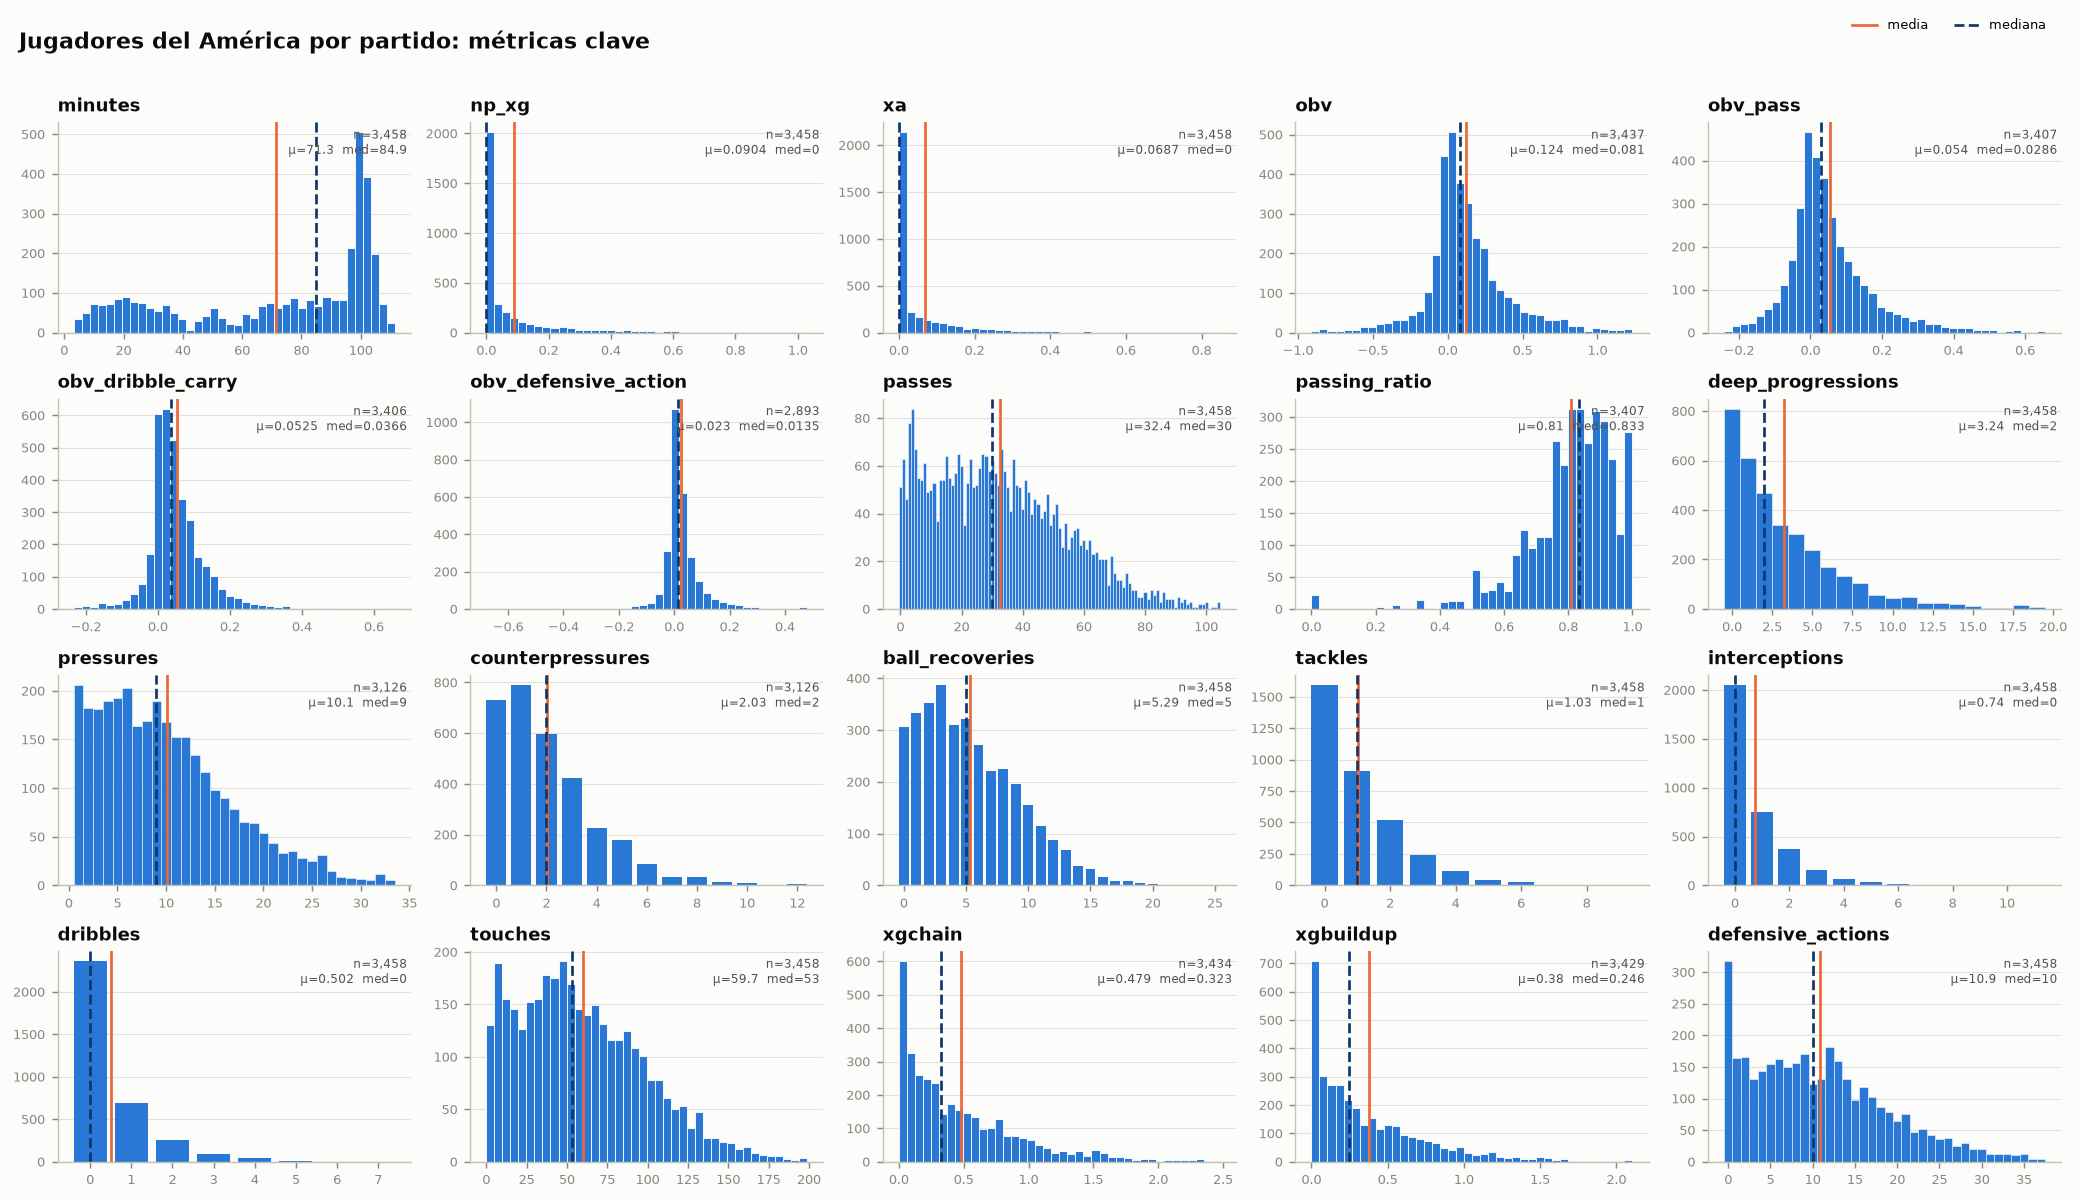
\includegraphics[width=\linewidth]{player_numericas_clave}
\caption{Métricas por jugador y partido. Los minutos son bimodales (titulares y suplentes). La producción ofensiva está inflada en ceros: el 51\% de las apariciones tiene np xG = 0.}
\end{figure}
\begin{table}[H]
\centering
\small
\caption{Jugadores con más minutos (2021--2026) y su OBV por 90 minutos.}
\label{tab:player_min}
\resizebox{\ifdim\width>\linewidth\linewidth\else\width\fi}{!}{%
\begin{tabular}{lrrr}
\toprule
\textbf{Jugador} & \textbf{Partidos} & \textbf{Minutos} & \textbf{OBV/90} \\
\midrule
Álvaro Fidalgo Fernández & 184 & 15,977 & 0.29 \\
Alejandro Zendejas Saavedra & 165 & 12,629 & 0.24 \\
Sebastián Enzo Cáceres Ramos & 139 & 12,513 & 0.10 \\
Henry Josué Martín Mex & 167 & 12,149 & 0.04 \\
Luis Ángel Malagón Velázquez & 120 & 12,102 & 0.06 \\
Israel Reyes Romero & 125 & 11,331 & 0.19 \\
Diego Alfonso Valdés Contreras & 124 & 9,190 & 0.18 \\
Richard Rafael Sánchez Guerrero & 128 & 8,458 & 0.24 \\
Kevin Nahin Álvarez Campos & 103 & 8,182 & 0.20 \\
Jonathan dos Santos Ramírez & 137 & 8,016 & 0.15 \\
Ramón Juárez Del Castillo & 102 & 7,880 & 0.06 \\
Paul Brian Rodríguez Bravo & 127 & 7,848 & 0.31 \\
Luis Fernando Fuentes Vargas & 92 & 7,153 & 0.25 \\
Cristian Alexis Borja González & 76 & 6,104 & 0.20 \\
Salvador Reyes Chávez & 99 & 6,020 & 0.18 \\
\bottomrule
\end{tabular}}
\end{table}
Álvaro Fidalgo es el eje del periodo (184 partidos, unos 16,000 minutos). Por la gran cantidad de ceros y porque todo depende de los minutos, \textbf{las métricas de jugador deben normalizarse por 90 minutos} y filtrarse con un mínimo de minutos.

\subsection{Alineaciones (\col{lineups})}
Cada fila es un convocado por partido. Trae datos personales (altura, peso, nacionalidad) y columnas anidadas: \col{positions} (posiciones jugadas con minuto de entrada y salida y su razón), \col{formations}, \col{stats} (goles y asistencias) y \col{events} (tarjetas).
\begin{table}[H]
\centering
\scriptsize
\caption{Posiciones jugadas y razones de entrada/salida (América).}
\label{tab:lineups_pos}
\resizebox{\ifdim\width>\linewidth\linewidth\else\width\fi}{!}{%
\begin{tabular}{lrrlrp{7.2cm}}
\toprule
\textbf{Columna} & \textbf{n} & \textbf{Cat.} & \textbf{Moda} & \textbf{\% moda} & \textbf{Top-8 (\%)} \\
\midrule
position & 4,672 & 23 & Right Defensive Midfield & 8.01 & Right Defensive Midfield (8.0\%) | Left Defensive Midfield (8.0\%) | Left Center Back (7.3\%) | Right Wing (7.1\%) | Center Forward (7.0\%) | Left Wing (6.8\%) | Right Center Back (6.7\%) | Left Back (6.1\%) \\
start\_reason & 4,672 & 7 & Starting XI & 52.27 & Starting XI (52.3\%) | Tactical Shift (23.1\%) | Substitution - On (Tactical) (19.3\%) | Player On (2.5\%) | Substitution - On (Injury) (1.7\%) | Substitution - On (Off Camera) (0.7\%) | Player On (Off Camera) (0.4\%) \\
end\_reason & 4,672 & 9 & Final Whistle & 51.82 & Final Whistle (51.8\%) | Tactical Shift (23.1\%) | Substitution - Off (Tactical) (19.3\%) | Player Off (2.8\%) | Substitution - Off (Injury) (1.7\%) | Substitution - Off (Off Camera) (0.7\%) | Red Card (0.3\%) | Second Yellow Card (0.1\%) \\
\bottomrule
\end{tabular}}
\end{table}
\begin{figure}[H]\centering
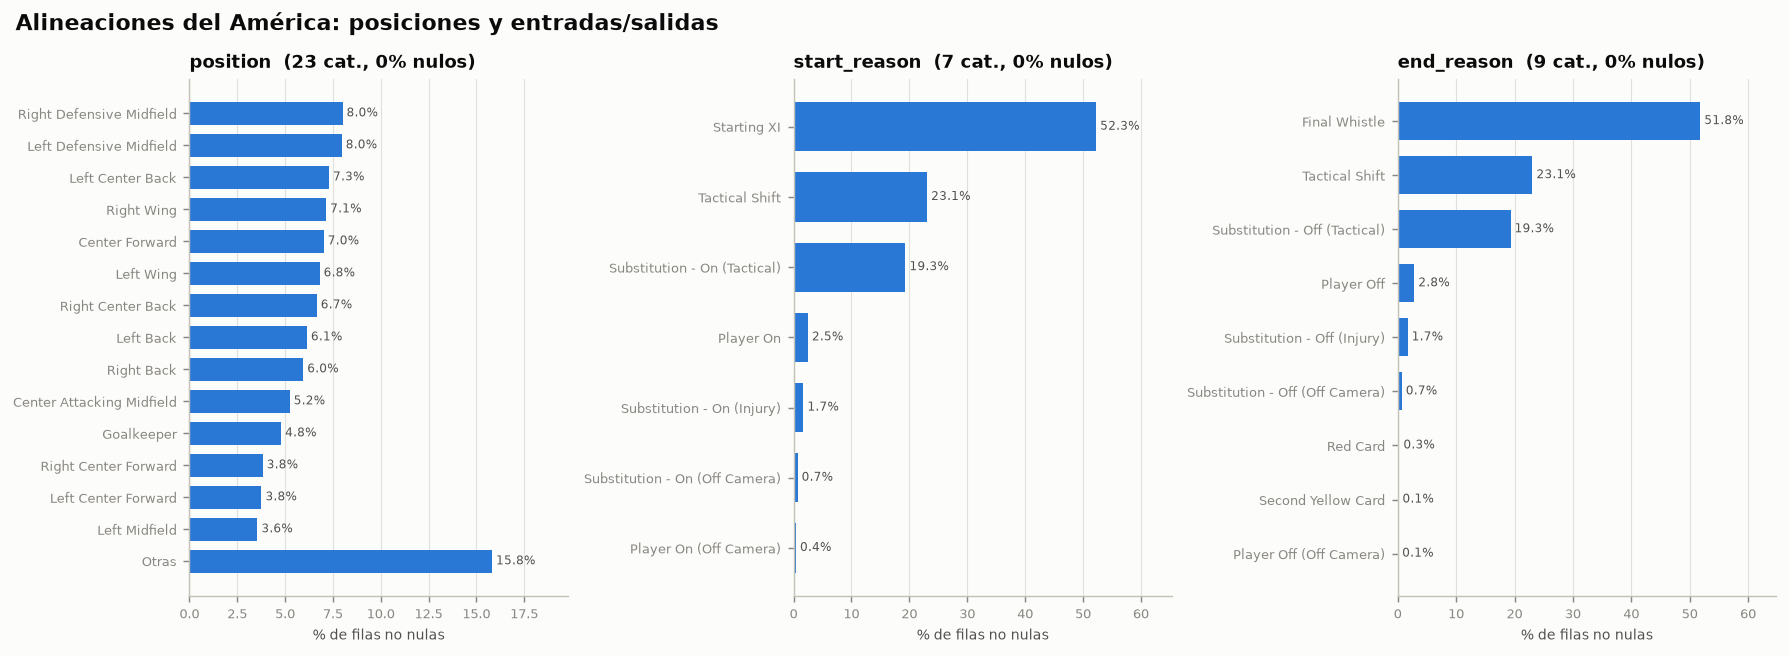
\includegraphics[width=\linewidth]{lineups_posiciones}
\caption{Posiciones del América y razones de entrada y salida. Los dos mediocampistas defensivos son las posiciones más ocupadas (doble pivote).}
\end{figure}
El 23\% de los tramos de posición empieza por un \emph{Tactical Shift}, es decir, un jugador que cambia de posición sin salir del campo. Esto indica que los sistemas cambian con frecuencia durante los partidos.

\begin{table}[H]
\centering
\small
\caption{Formación inicial (evento \texttt{Starting XI}) por entrenador.}
\label{tab:formaciones}
\resizebox{\ifdim\width>\linewidth\linewidth\else\width\fi}{!}{%
\begin{tabular}{lrrrrrr}
\toprule
\textbf{Formación} & \textbf{Jardine} & \textbf{Cervantes} & \textbf{Ortiz} & \textbf{Almada} & \textbf{Solari} & \textbf{All} \\
\midrule
3-4-1-2 & 0 & 0 & 1 & 0 & 0 & 1 \\
3-4-2-1 & 8 & 1 & 0 & 0 & 0 & 9 \\
3-4-3 & 14 & 0 & 0 & 0 & 1 & 15 \\
3-5-2 & 5 & 0 & 0 & 0 & 1 & 6 \\
4-1-2-1-2 & 1 & 0 & 1 & 0 & 1 & 3 \\
4-1-4-1 & 7 & 0 & 0 & 0 & 3 & 10 \\
4-2-3-1 & 57 & 1 & 33 & 8 & 12 & 111 \\
4-3-3 & 9 & 0 & 2 & 0 & 2 & 13 \\
4-4-1-1 & 2 & 0 & 1 & 0 & 0 & 3 \\
4-4-2 & 26 & 0 & 17 & 1 & 6 & 50 \\
4-5-1 & 0 & 0 & 0 & 0 & 1 & 1 \\
Total & 129 & 2 & 55 & 9 & 27 & 222 \\
\bottomrule
\end{tabular}}
\end{table}
El 4-2-3-1 es la base del club (111 de 222 partidos). Jardine usó \textbf{nueve formaciones iniciales} distintas, 27 de sus partidos con línea de tres (3-4-3, 3-4-2-1, 3-5-2).

\subsection{StatsBomb 360 (\col{frames360})}
Cada fila es un jugador visible en el cuadro de un evento: \col{teammate}, \col{actor}, \col{keeper}, \col{location} y el polígono \col{visible_area}.
\begin{table}[H]
\centering
\small
\caption{Jugadores visibles por evento en StatsBomb 360 (muestra de 20 partidos).}
\label{tab:frames360}
\resizebox{\ifdim\width>\linewidth\linewidth\else\width\fi}{!}{%
\begin{tabular}{lrrrrrrrr}
\toprule
\textbf{Variable} & \textbf{Eventos} & \textbf{Mín} & \textbf{P25} & \textbf{Mediana} & \textbf{Media} & \textbf{P75} & \textbf{Máx} & \textbf{Desv.} \\
\midrule
jugadores visibles & 60,540 & 1 & 11 & 14 & 13.52 & 16 & 22 & 4.08 \\
compañeros & 60,540 & 0 & 5 & 7 & 6.76 & 8 & 11 & 2.14 \\
rivales & 60,540 & 0 & 5 & 7 & 6.77 & 9 & 11 & 2.46 \\
\bottomrule
\end{tabular}}
\end{table}
\begin{figure}[H]\centering
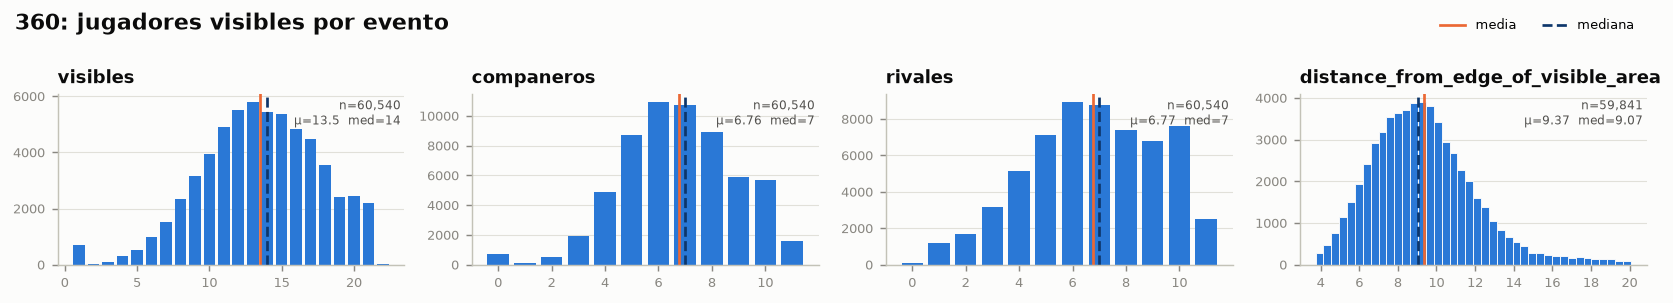
\includegraphics[width=\linewidth]{frames360_visibles}
\caption{Jugadores visibles por evento: mediana de 14, con compañeros y rivales equilibrados.}
\end{figure}

% =====================================================================
\section{Relaciones entre variables}\label{sec:relaciones}
% =====================================================================
\subsection{Eventos: variables categóricas}
\begin{figure}[H]\centering
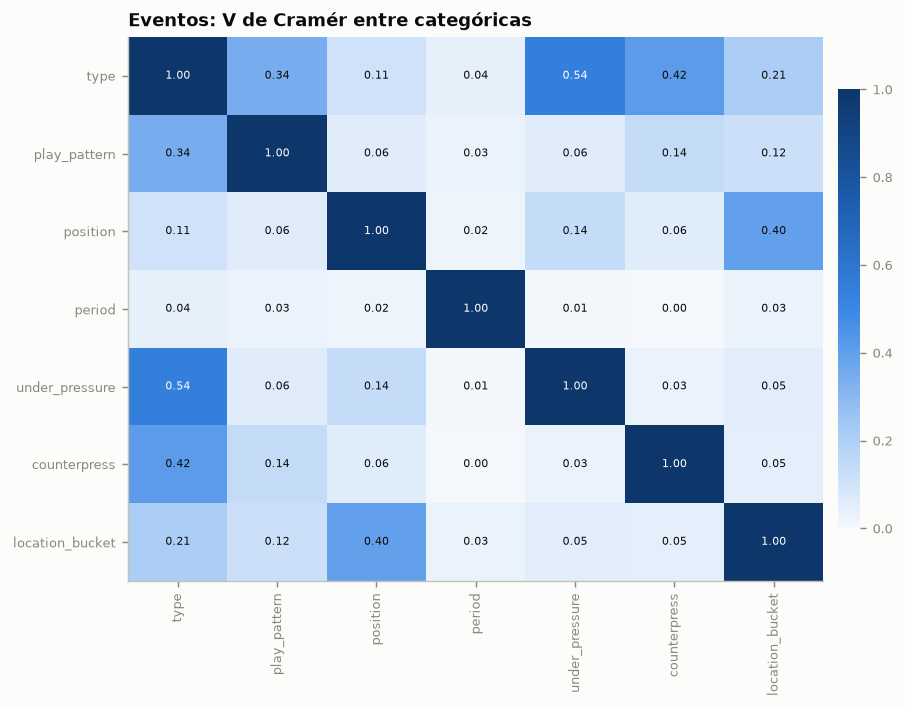
\includegraphics[width=0.49\linewidth]{events_cramers_v}\hfill
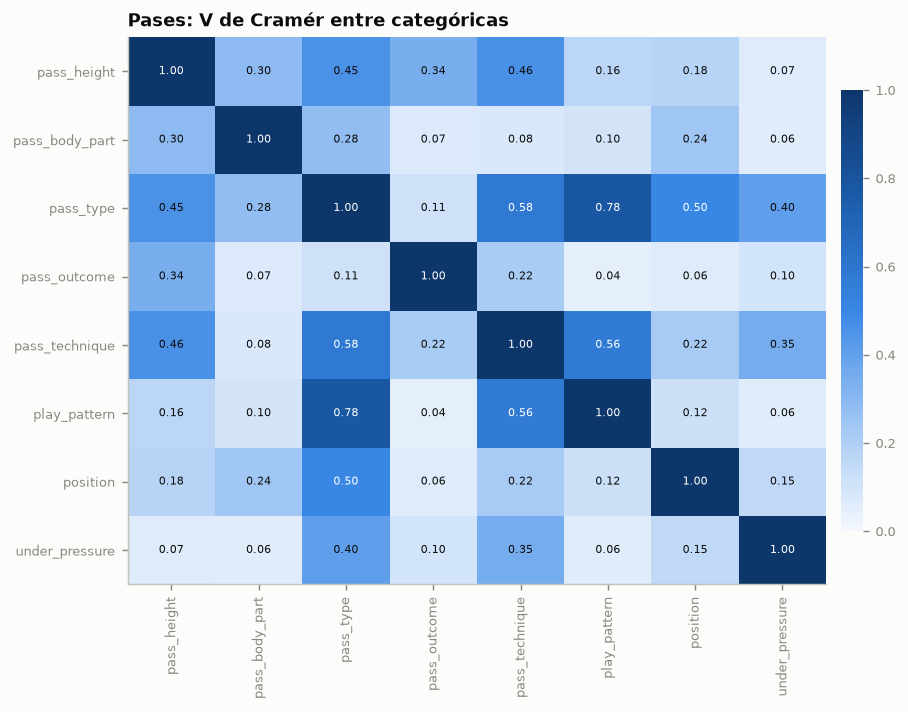
\includegraphics[width=0.49\linewidth]{events_pases_cramers_v}
\caption{V de Cramér entre variables categóricas de eventos (izquierda) y de pases (derecha).}\label{fig:cramer}
\end{figure}
\begin{itemize}
  \item \col{type} se asocia con \col{under_pressure} ($V=0.54$) y \col{counterpress} ($0.42$): ciertas acciones (recepciones, conducciones, duelos) ocurren bajo presión con mucha más frecuencia.
  \item \col{position} se asocia con \col{location_bucket} ($0.40$): cada posición ocupa zonas claras, lo que permite estudiar roles espaciales.
  \item En pases, \col{pass_type} y \col{play_pattern} están muy asociados ($0.78$) porque ambos codifican la reanudación. En el marco analítico conviene usar solo una de las dos.
  \item \col{pass_height} se asocia con \col{pass_outcome} ($0.34$): los pases altos fallan más.
\end{itemize}

\subsection{Eventos: variables numéricas}
\begin{figure}[H]\centering
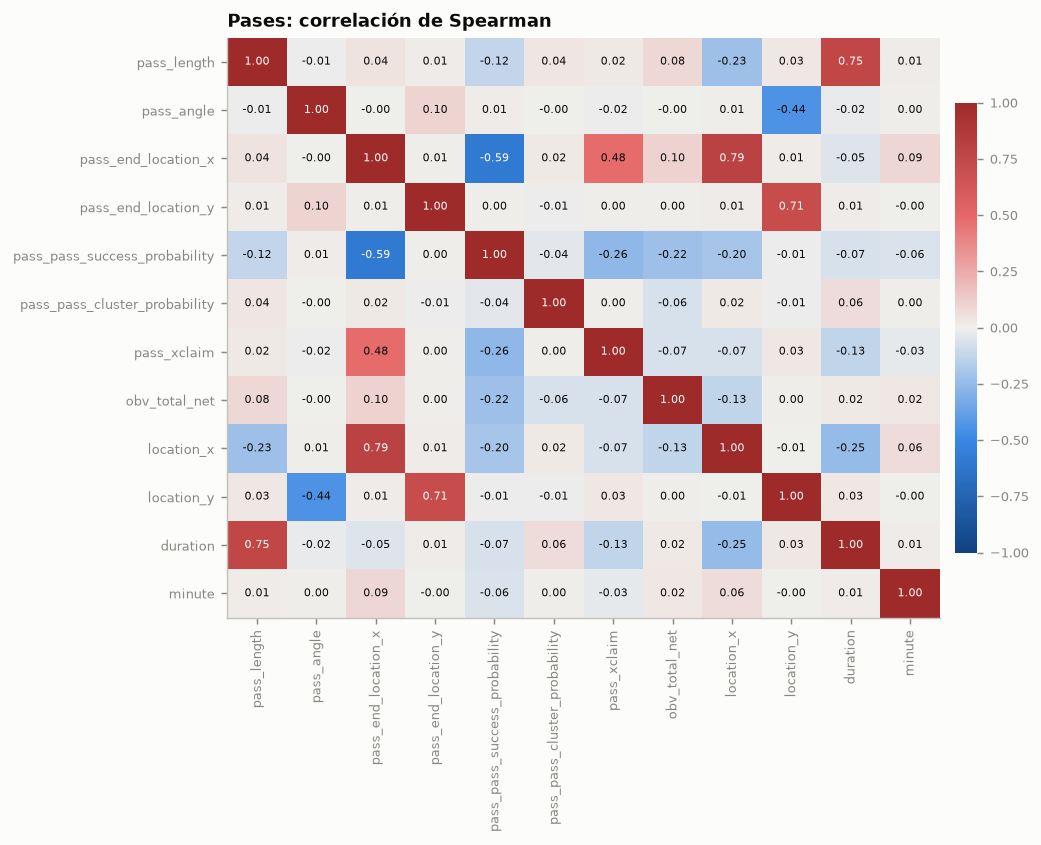
\includegraphics[width=0.49\linewidth]{events_pases_correlacion}\hfill
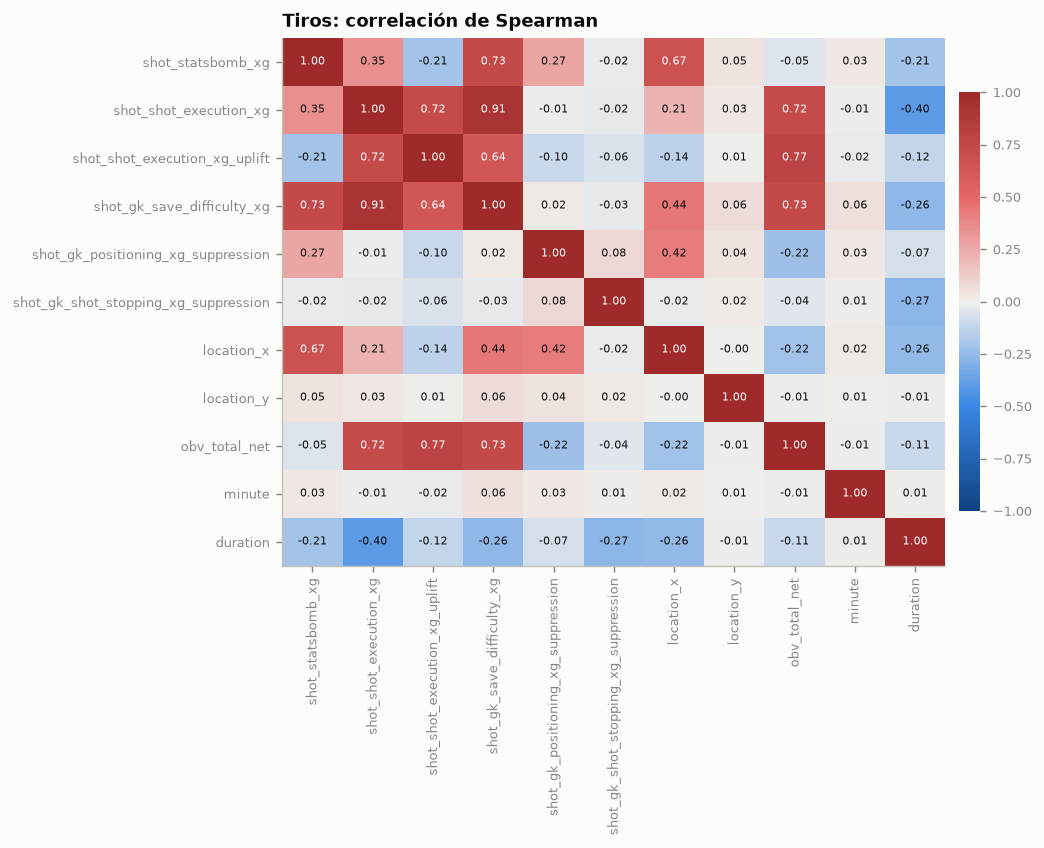
\includegraphics[width=0.49\linewidth]{events_tiros_correlacion}
\caption{Correlación de Spearman en pases (izquierda) y tiros (derecha).}\label{fig:corr_events}
\end{figure}
\begin{itemize}
  \item \textbf{Riesgo y progresión}: la probabilidad de éxito de un pase baja cuanto más adelante termina ($\rho=-0.59$ con \col{pass_end_location_x}). Por construcción, \emph{progresar es arriesgar}, lo que abre la pregunta de cuánto riesgo asume cada entrenador.
  \item Los pases largos duran más ($\rho=0.75$), y la $x$ final del pase depende sobre todo de la inicial ($0.79$).
  \item En tiros, el xG aumenta con la cercanía a la portería ($\rho=0.67$ con $x$), y el xG de ejecución está muy ligado a la dificultad de atajada ($0.91$).
\end{itemize}

\subsection{Métricas de equipo}
\begin{figure}[H]\centering
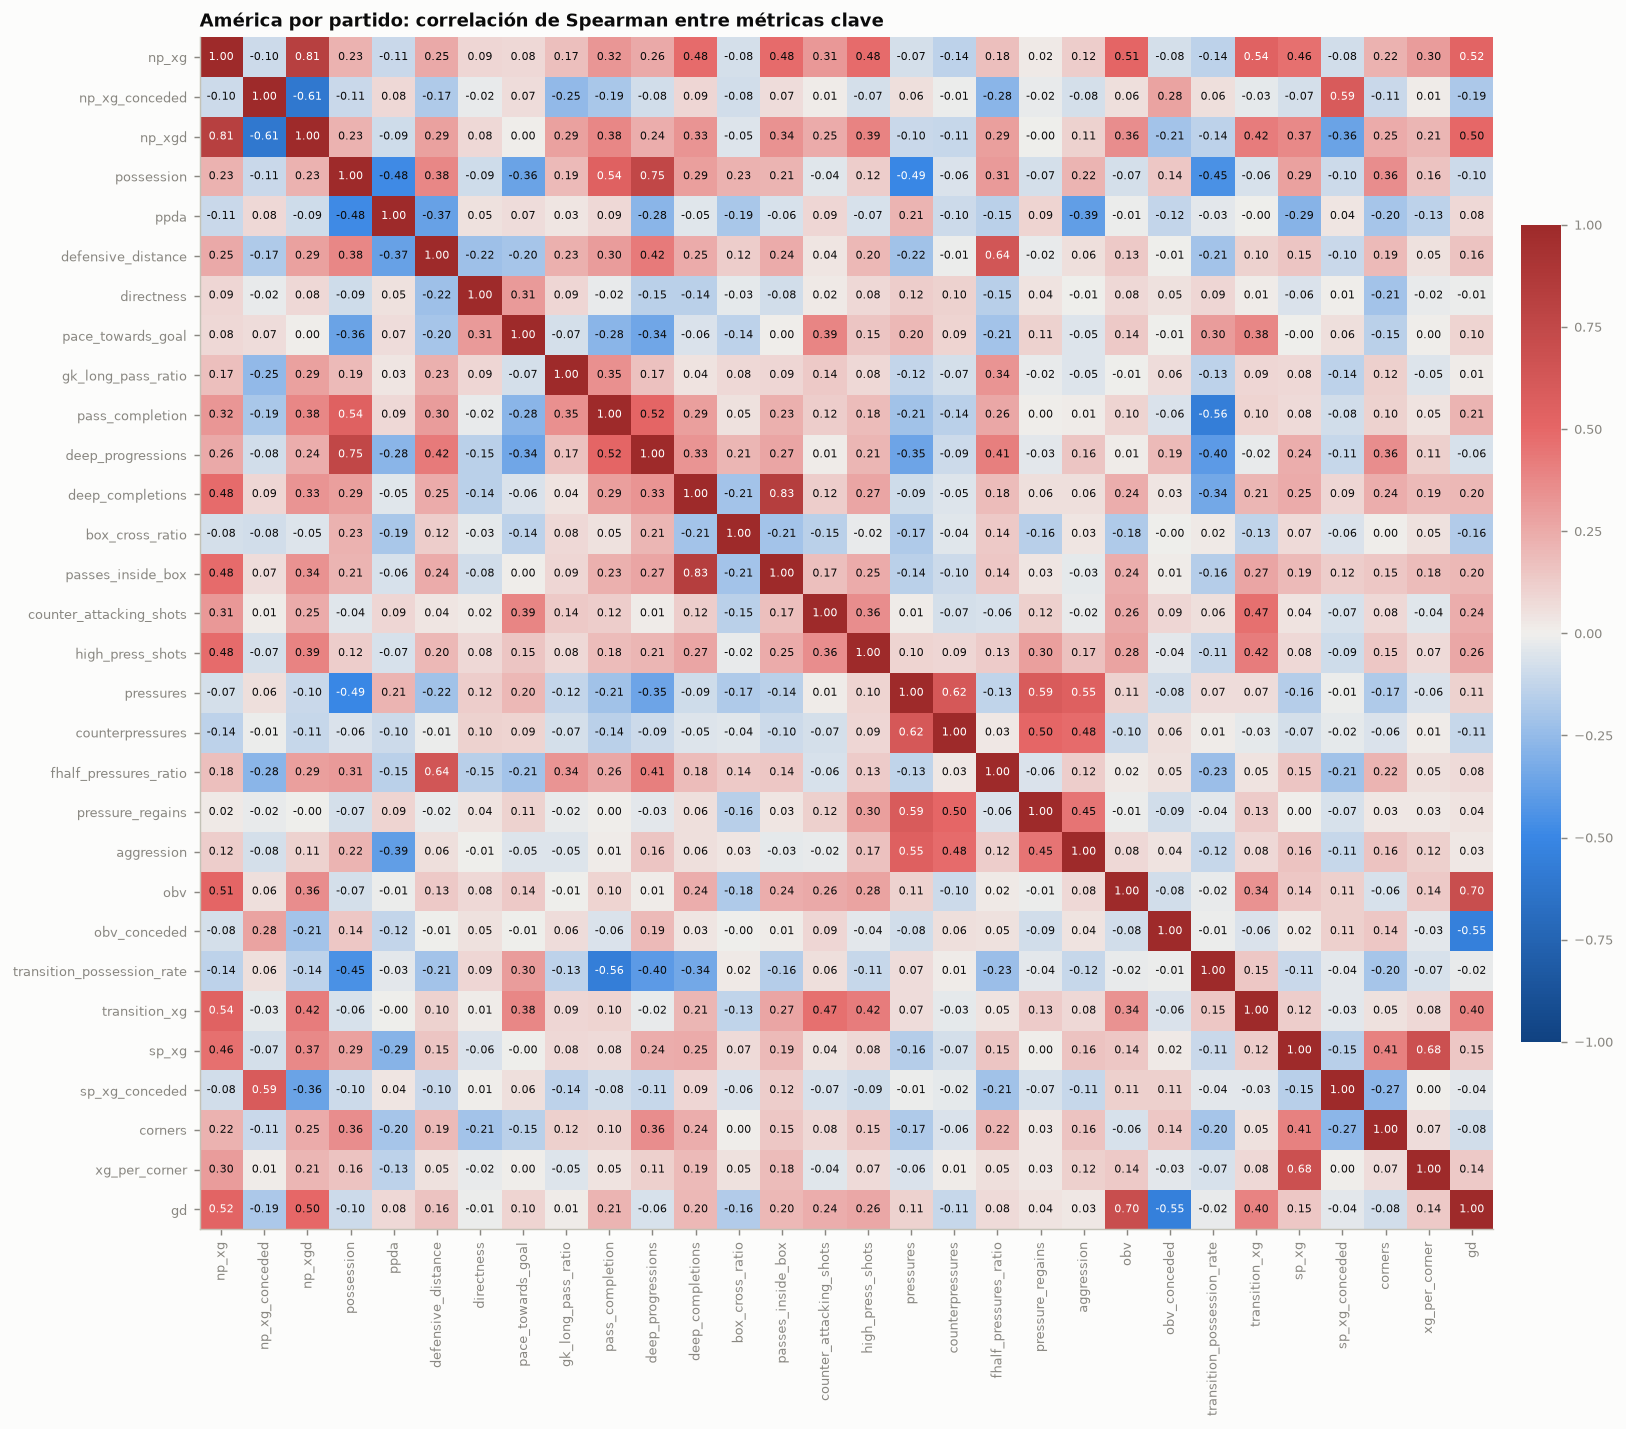
\includegraphics[width=\linewidth]{team_correlacion_clave}
\caption{Correlación de Spearman entre métricas clave del América por partido.}\label{fig:team_corr}
\end{figure}
La Figura~\ref{fig:team_corr} muestra \textbf{bloques de métricas} que se mueven juntas:
\begin{itemize}
  \item \textbf{Dominio con balón}: la posesión se relaciona con las progresiones profundas ($\rho=0.75$), con el field tilt ($0.82$), con la precisión de pase ($0.54$) y con una línea defensiva más alta (\col{defensive_distance}, $0.38$).
  \item \textbf{Presión}: presiones, contrapresiones, recuperaciones tras presión y agresividad forman un bloque ($\rho$ entre 0.45 y 0.62). La posesión se relaciona \emph{negativamente} con el PPDA ($-0.48$) y con el número de presiones ($-0.49$): quien tiene el balón presiona menos veces, pero con más intensidad relativa.
  \item \textbf{Altura del bloque}: \col{defensive_distance} está muy ligada al \% de presiones en campo rival ($0.64$).
  \item \textbf{Transición contra control}: la tasa de posesiones de transición se relaciona negativamente con la posesión ($-0.45$) y con la precisión ($-0.56$).
  \item \textbf{Balón parado}: el xG de balón parado depende de la calidad del córner ($0.68$ con xG por córner), y el xG concedido depende en buena parte del balón parado rival ($0.59$).
\end{itemize}

\begin{table}[H]
\centering
\scriptsize
\caption{Pares de métricas de equipo con mayor correlación de Spearman: redundancias por construcción.}
\label{tab:team_top_corr}
\resizebox{\ifdim\width>\linewidth\linewidth\else\width\fi}{!}{%
\begin{tabular}{llr}
\toprule
\textbf{Variable 1} & \textbf{Variable 2} & \textbf{$\rho$} \\
\midrule
opp\_final\_third\_pass\_ratio & passing\_ratio & 1.00 \\
goals\_from\_throw\_ins\_conceded & throw\_in\_goal\_ratio\_conceded & 1.00 \\
goals\_conceded & goals\_against & 1.00 \\
goals\_from\_throw\_ins & throw\_in\_goal\_ratio & 1.00 \\
direct\_free\_kick\_goals\_conceded & direct\_free\_kick\_goal\_ratio\_conceded & 1.00 \\
throw\_in\_xg & xg\_per\_throw\_in & 1.00 \\
throw\_in\_xg\_conceded & xg\_per\_throw\_in\_conceded & 1.00 \\
goals\_from\_indirect\_free\_kicks & indirect\_free\_kick\_goal\_ratio & 1.00 \\
goals\_from\_indirect\_free\_kicks\_conceded & indirect\_free\_kick\_goal\_ratio\_conceded & 1.00 \\
goals\_from\_free\_kicks\_conceded & free\_kick\_goal\_ratio\_conceded & 1.00 \\
shots\_from\_throw\_ins & throw\_in\_shot\_ratio & 1.00 \\
throw\_in\_xg & shots\_from\_throw\_ins & 1.00 \\
xg\_per\_throw\_in & shots\_from\_throw\_ins & 1.00 \\
goals\_from\_free\_kicks & free\_kick\_goal\_ratio & 1.00 \\
goals\_from\_corners & corner\_goal\_ratio & 1.00 \\
\bottomrule
\end{tabular}}
\end{table}
Muchas de las 199 métricas son \textbf{redundantes por construcción} (conteo contra ratio, total contra juego abierto, $\rho\approx1$). Antes de cualquier modelo hay que elegir una sola métrica por familia.

\begin{table}[H]
\centering
\small
\caption{Métricas de equipo más asociadas a la diferencia de goles del partido (Spearman).}
\label{tab:team_gd}
\resizebox{\ifdim\width>\linewidth\linewidth\else\width\fi}{!}{%
\begin{tabular}{lr}
\toprule
\textbf{Métrica} & \textbf{$\rho$ con diferencia de goles} \\
\midrule
goals\_for & 0.77 \\
obv & 0.70 \\
goals\_against & -0.60 \\
obv\_conceded & -0.55 \\
xgd & 0.54 \\
op\_xg & 0.54 \\
np\_xg & 0.52 \\
np\_xgd & 0.50 \\
obv\_shot & 0.46 \\
np\_xg\_per\_shot & 0.44 \\
shots\_in\_clear & 0.44 \\
transition\_xg & 0.40 \\
sp\_goal\_ratio\_conceded & -0.37 \\
obv\_gk & 0.37 \\
sp\_goals\_conceded & -0.37 \\
op\_shots & 0.36 \\
obv\_gk\_conceded & -0.35 \\
corner\_goal\_ratio\_conceded & -0.34 \\
\bottomrule
\end{tabular}}
\end{table}
\paragraph{¿Qué métricas acompañan al resultado?} \textbf{OBV} ($\rho=0.70$) se asocia con la diferencia de goles más que el xG diferencial ($0.54$) o el np xG ($0.52$). OBV mide el valor de \emph{todas} las acciones con balón y no solo de los tiros, así que es un buen candidato para medir el ``dominio'' en la narrativa. La posesión casi no se asocia con el resultado ($\rho=-0.10$).

\subsection{Métricas de jugador}
\begin{figure}[H]\centering
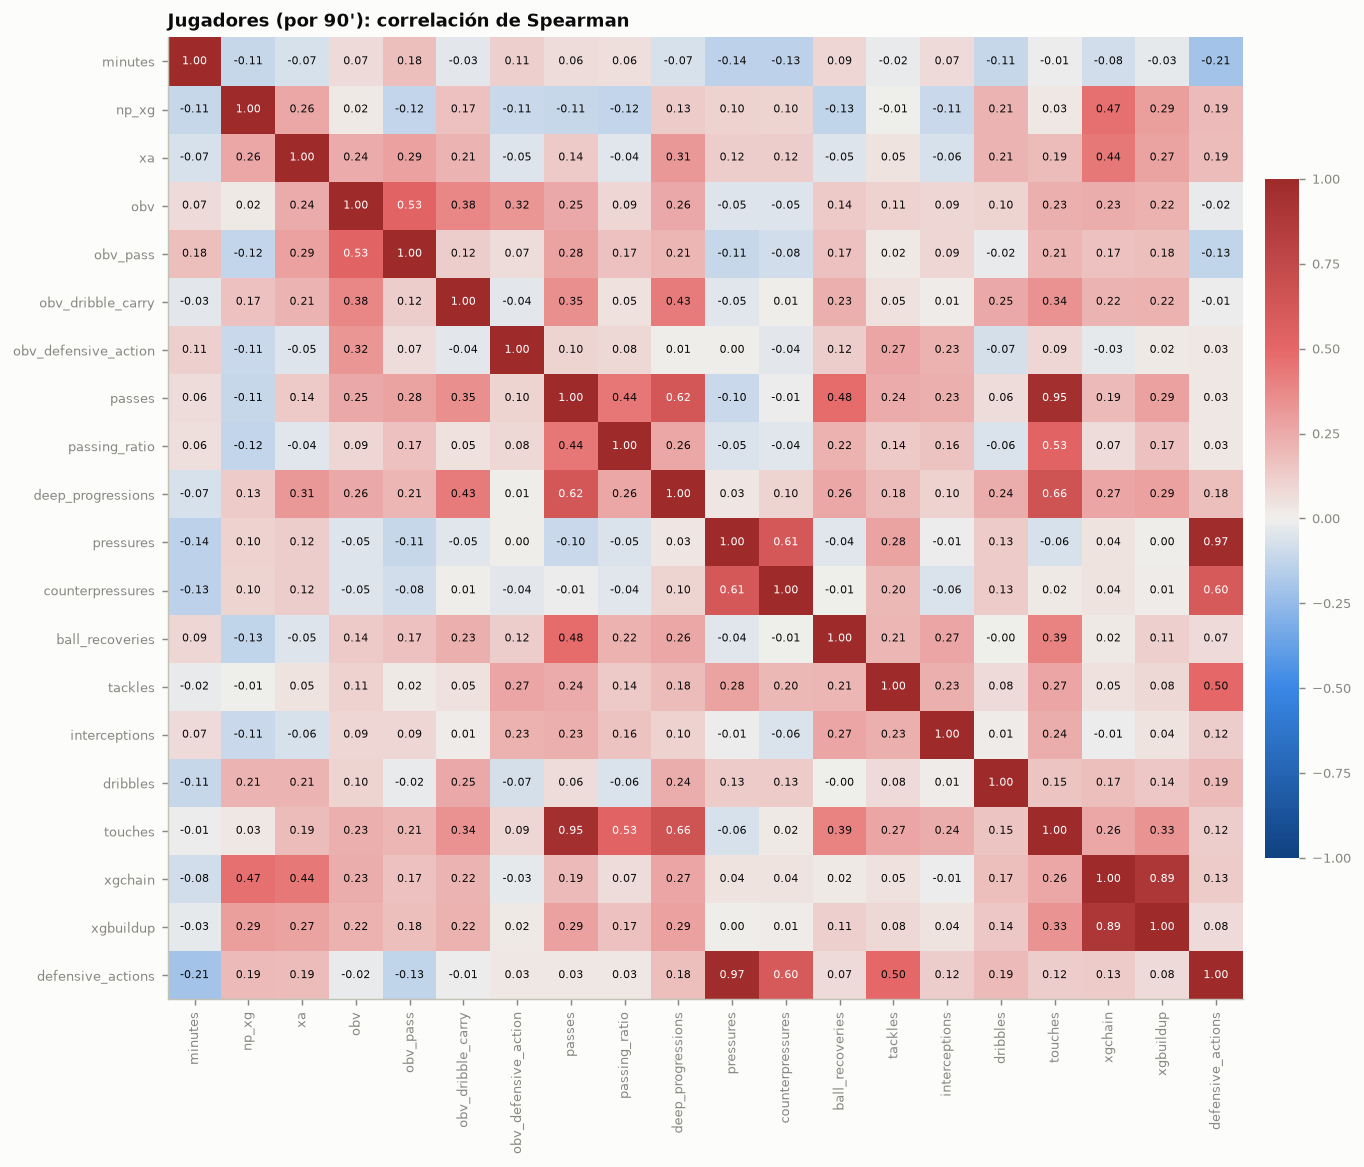
\includegraphics[width=0.85\linewidth]{player_correlacion_p90}
\caption{Correlación de Spearman entre métricas de jugador por 90 minutos (jugadores con 30 minutos o más).}
\end{figure}
Por 90 minutos se ven perfiles que no se mezclan. El perfil de \emph{organizador} agrupa pases, toques y progresiones profundas ($\rho$ entre 0.62 y 0.95). El de \emph{presionador} agrupa presiones y acciones defensivas ($0.97$, porque las acciones defensivas incluyen las presiones). El de \emph{finalizador} agrupa np xG y xGChain ($0.47$). Estos perfiles sugieren usar una tipología de roles para analizar el uso de jugadores.

% =====================================================================
\section{Relación con el contexto}\label{sec:contexto}
% =====================================================================
Esta sección cruza las métricas por partido con los contextos que pide el reto. Primero se presentan las métricas derivadas.
\begin{table}[H]
\centering
\small
\caption{Métricas derivadas de eventos (definiciones en la Sección~\ref{sec:metodologia}).}
\label{tab:ctx_new}
\resizebox{\ifdim\width>\linewidth\linewidth\else\width\fi}{!}{%
\begin{tabular}{lrrrrrrrr}
\toprule
\textbf{Métrica} & \textbf{n} & \textbf{Mín} & \textbf{P25} & \textbf{Mediana} & \textbf{Media} & \textbf{P75} & \textbf{Máx} & \textbf{Desv.} \\
\midrule
field\_tilt & 222 & 0.14 & 0.50 & 0.61 & 0.60 & 0.72 & 0.91 & 0.15 \\
progressive\_passes & 222 & 13.00 & 27.25 & 35.00 & 35.04 & 41.00 & 62.00 & 9.97 \\
progressive\_passes\_rival & 222 & 10.00 & 22.00 & 27.00 & 27.89 & 33.00 & 54.00 & 8.58 \\
pass\_x\_mean & 222 & 42.00 & 55.66 & 58.59 & 58.60 & 62.06 & 72.95 & 4.88 \\
pressure\_x\_mean & 222 & 44.02 & 53.50 & 57.93 & 57.74 & 61.50 & 72.05 & 5.52 \\
\bottomrule
\end{tabular}}
\end{table}

\subsection{Tiempo: evolución partido a partido y por torneo}
\begin{figure}[H]\centering
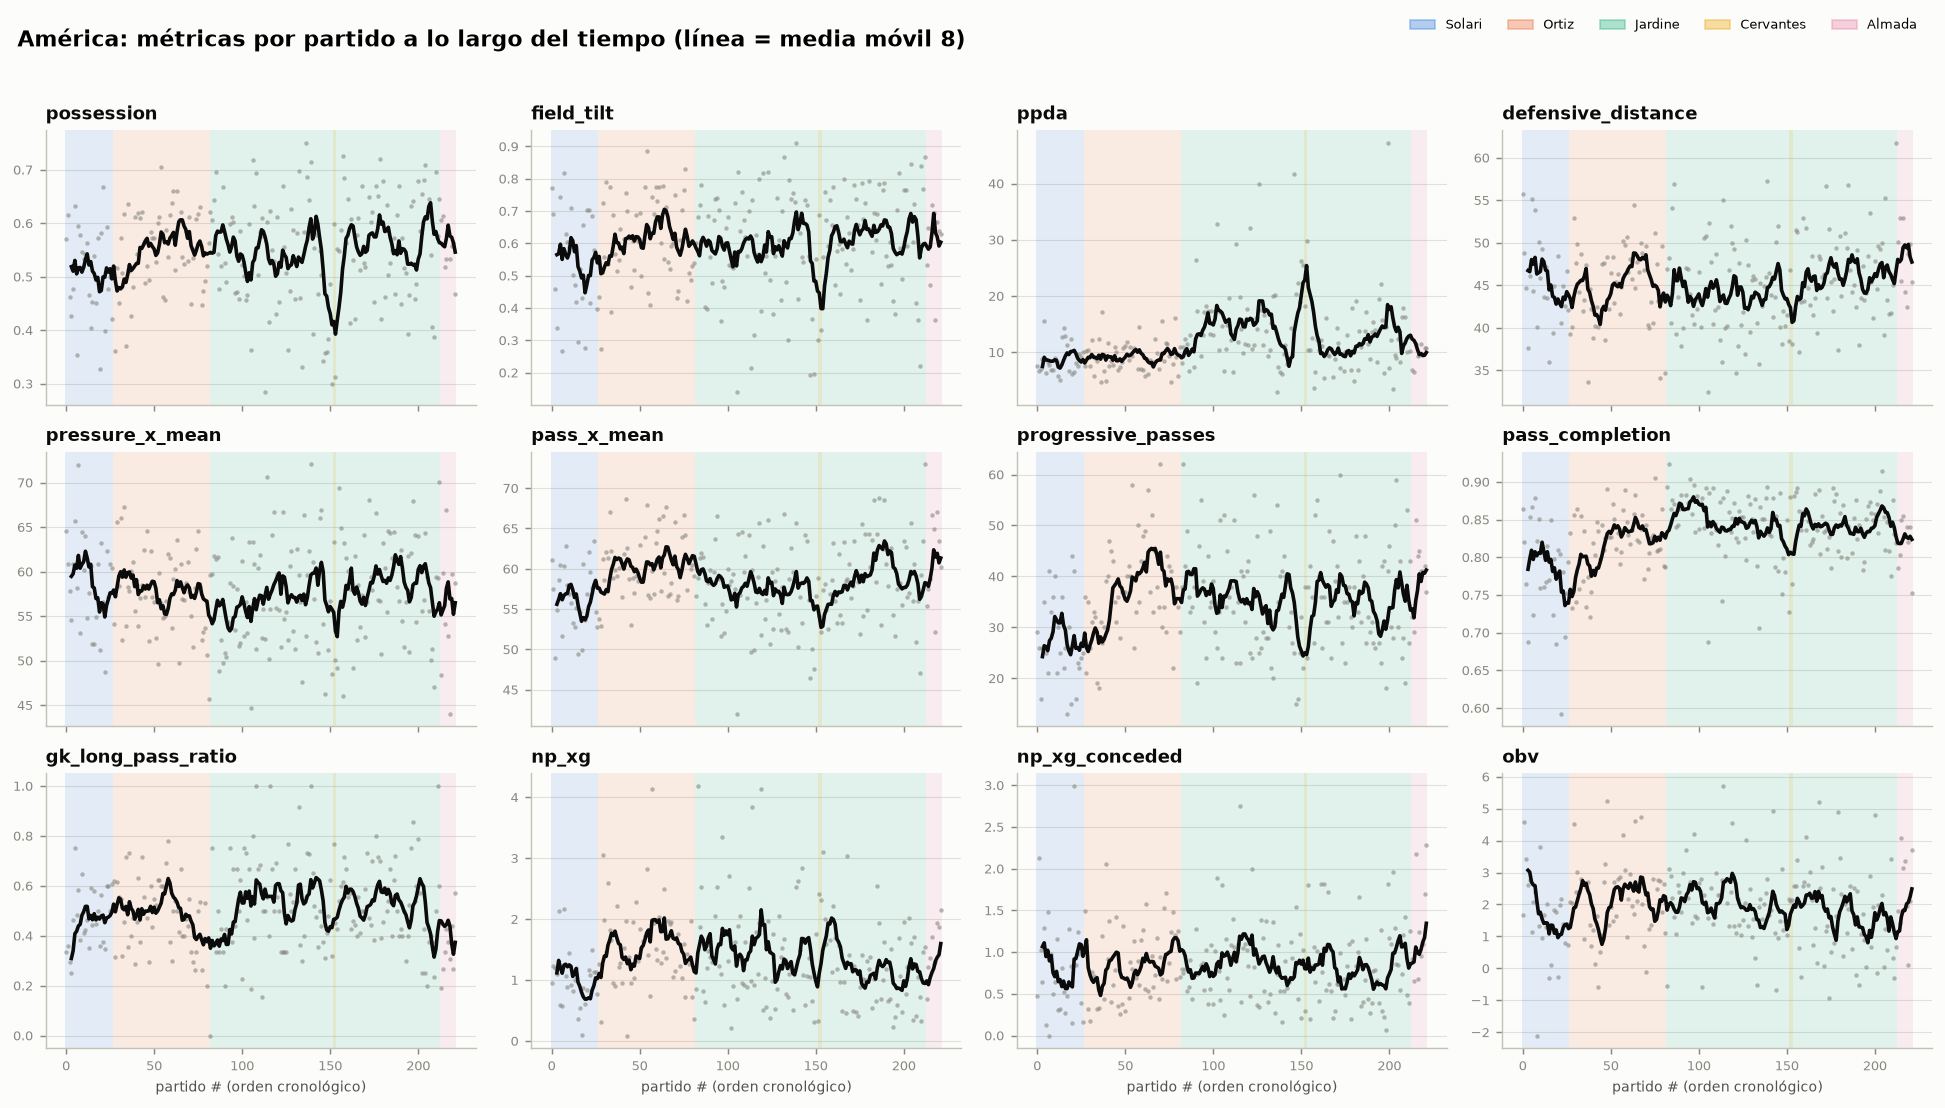
\includegraphics[width=\linewidth]{contexto_series_tiempo}
\caption{Métricas del América por partido en orden cronológico. La línea es la media móvil de 8 partidos y el fondo indica el entrenador.}\label{fig:series}
\end{figure}
\begin{table}[H]
\centering
\scriptsize
\caption{Evolución por torneo (medianas por partido).}
\label{tab:ctx_torneo}
\resizebox{\ifdim\width>\linewidth\linewidth\else\width\fi}{!}{%
\begin{tabular}{lrrrrrrrrrrr}
\toprule
\textbf{Torneo · entrenador} & \textbf{Posesión} & \textbf{Field tilt} & \textbf{PPDA} & \textbf{x presión} & \textbf{Pases prog.} & \textbf{Precisión} & \textbf{Saque largo GK} & \textbf{np xG} & \textbf{np xG c.} & \textbf{n} & \textbf{\% G} \\
\midrule
Apertura 2021 · Solari & 0.54 & 0.58 & 7.69 & 60.14 & 26.00 & 0.81 & 0.45 & 0.95 & 0.64 & 19 & 53 \\
Clausura 2022 · Solari & 0.49 & 0.57 & 8.67 & 58.81 & 23.50 & 0.77 & 0.53 & 1.10 & 0.84 & 8 & 12 \\
Clausura 2022 · Ortiz & 0.51 & 0.56 & 8.39 & 58.29 & 31.00 & 0.77 & 0.47 & 1.45 & 0.69 & 13 & 54 \\
Apertura 2022 · Ortiz & 0.57 & 0.62 & 9.38 & 57.08 & 40.00 & 0.83 & 0.56 & 1.52 & 0.79 & 21 & 67 \\
Clausura 2023 · Ortiz & 0.55 & 0.59 & 8.73 & 57.70 & 38.00 & 0.82 & 0.42 & 1.43 & 0.88 & 21 & 52 \\
Apertura 2023 · Jardine & 0.53 & 0.61 & 13.12 & 56.61 & 38.00 & 0.87 & 0.45 & 1.34 & 0.76 & 23 & 65 \\
Clausura 2024 · Jardine & 0.55 & 0.58 & 14.12 & 55.81 & 35.00 & 0.84 & 0.50 & 1.03 & 1.03 & 23 & 52 \\
Apertura 2024 · Jardine & 0.53 & 0.59 & 12.51 & 56.67 & 30.50 & 0.85 & 0.50 & 1.14 & 0.75 & 24 & 50 \\
Clausura 2025 · Cervantes & 0.46 & 0.51 & 24.07 & 56.70 & 31.00 & 0.82 & 0.61 & 2.36 & 0.61 & 2 & 50 \\
Clausura 2025 · Jardine & 0.58 & 0.63 & 10.33 & 58.45 & 36.00 & 0.84 & 0.54 & 1.26 & 0.65 & 21 & 52 \\
Apertura 2025 · Jardine & 0.55 & 0.64 & 11.86 & 59.77 & 32.00 & 0.84 & 0.50 & 1.02 & 0.73 & 19 & 58 \\
Clausura 2026 · Jardine & 0.61 & 0.68 & 12.40 & 59.35 & 30.00 & 0.85 & 0.50 & 1.04 & 0.85 & 19 & 37 \\
Apertura 2026 · Almada & 0.56 & 0.64 & 9.76 & 55.90 & 41.00 & 0.83 & 0.33 & 1.36 & 1.10 & 9 & 67 \\
\bottomrule
\end{tabular}}
\end{table}
\begin{itemize}
  \item \textbf{Precisión de pase}: sube por escalones de un entrenador a otro. Con Solari es de 0.77--0.81, con Ortiz de 0.83 y con Jardine de 0.84--0.87, el máximo del periodo.
  \item \textbf{PPDA}: se mantiene estable en 8--9 con Solari y Ortiz y \textbf{sube a 10--14 con Jardine}, con picos en la liguilla del Apertura 2024. Almada lo regresa a 9.8.
  \item \textbf{Salida del portero}: con Almada cae a 0.33 (más salida corta).
  \item \textbf{Field tilt}: con Jardine tiende a subir (0.61 en el Apertura 2023, 0.68 en el Clausura 2026), pero su xG propio baja (1.34 $\to$ 1.04) y el porcentaje de victorias cae en el Clausura 2026 (37\%).
\end{itemize}
En la Figura~\ref{fig:series} se ve un episodio muy marcado alrededor del partido 145: la posesión se desploma y el PPDA se dispara. Corresponde a la liguilla del Apertura 2024 (Sección~\ref{sec:fase}).

\subsection{Entrenador}
\begin{figure}[H]\centering
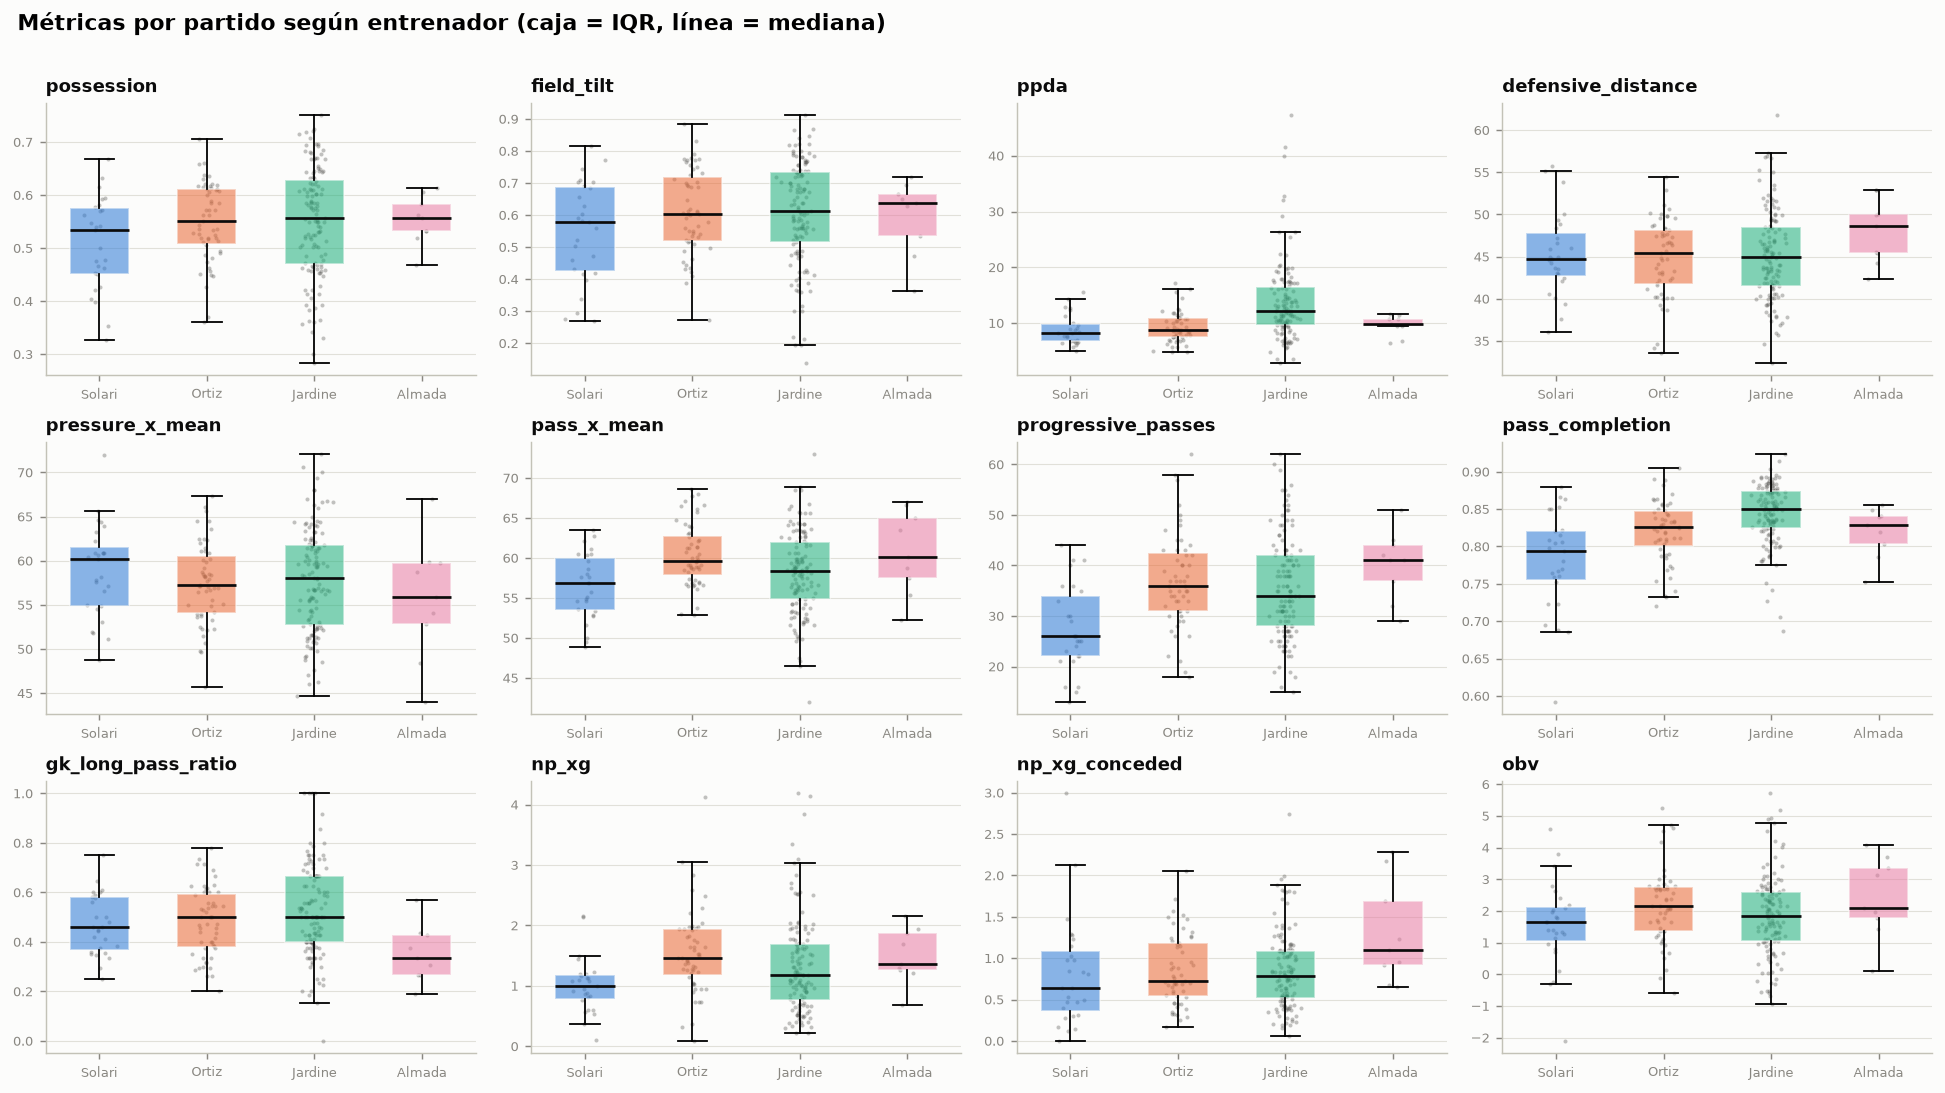
\includegraphics[width=\linewidth]{contexto_boxplots_entrenador}
\caption{Métricas por partido según entrenador. La caja es el rango intercuartílico, la línea la mediana y los puntos son partidos.}\label{fig:box}
\end{figure}
\begin{table}[H]
\centering
\scriptsize
\caption{Métricas por partido según entrenador: mediana [P25--P75].}
\label{tab:ctx_coach}
\resizebox{\ifdim\width>\linewidth\linewidth\else\width\fi}{!}{%
\begin{tabular}{lllll}
\toprule
\textbf{Métrica} & \textbf{Solari} & \textbf{Ortiz} & \textbf{Jardine} & \textbf{Almada} \\
\midrule
possession & 0.53 [0.45–0.58] & 0.55 [0.51–0.61] & 0.56 [0.47–0.63] & 0.56 [0.53–0.58] \\
field\_tilt & 0.58 [0.43–0.69] & 0.60 [0.52–0.72] & 0.61 [0.52–0.73] & 0.64 [0.53–0.67] \\
ppda & 8.18 [6.72–9.87] & 8.73 [7.50–10.97] & 12.15 [9.57–16.40] & 9.76 [9.42–10.77] \\
defensive\_distance & 44.72 [42.74–47.81] & 45.42 [41.77–48.20] & 44.94 [41.51–48.54] & 48.66 [45.38–50.11] \\
pressure\_x\_mean & 60.14 [54.88–61.59] & 57.26 [54.04–60.54] & 58.02 [52.72–61.76] & 55.90 [52.81–59.70] \\
pass\_x\_mean & 56.90 [53.46–59.96] & 59.68 [57.81–62.78] & 58.39 [54.91–62.02] & 60.16 [57.48–64.93] \\
progressive\_passes & 26.00 [22.00–34.00] & 36.00 [31.00–42.50] & 34.00 [28.00–42.00] & 41.00 [37.00–44.00] \\
pass\_completion & 0.79 [0.76–0.82] & 0.83 [0.80–0.85] & 0.85 [0.83–0.87] & 0.83 [0.80–0.84] \\
gk\_long\_pass\_ratio & 0.46 [0.37–0.58] & 0.50 [0.38–0.60] & 0.50 [0.40–0.67] & 0.33 [0.27–0.43] \\
np\_xg & 1.00 [0.79–1.18] & 1.46 [1.18–1.94] & 1.19 [0.76–1.70] & 1.36 [1.26–1.87] \\
np\_xg\_conceded & 0.65 [0.36–1.09] & 0.72 [0.54–1.18] & 0.78 [0.52–1.09] & 1.10 [0.91–1.69] \\
obv & 1.66 [1.05–2.13] & 2.15 [1.36–2.75] & 1.85 [1.06–2.59] & 2.09 [1.78–3.36] \\
partidos & 27 & 55 & 129 & 9 \\
\bottomrule
\end{tabular}}
\end{table}
\begin{itemize}
  \item La \textbf{posesión no separa a los entrenadores}: las medianas van de 0.53 a 0.56 y los rangos se traslapan casi por completo.
  \item El \textbf{PPDA sí los separa}. Jardine tiene la mediana más alta (12.2) y la mayor dispersión (IQR 9.6--16.4); Solari y Ortiz presionan de forma más intensa y más constante.
  \item La \textbf{precisión} crece de Solari a Jardine. Los \textbf{pases progresivos} suben de 26 con Solari a 34--41 con los demás.
  \item Almada tiene la línea más alta (\col{defensive_distance} 48.7) y la salida más corta del portero, pero también el mayor xG concedido (1.10). Con 9 partidos, estas diferencias son solo indicativas.
\end{itemize}

\begin{figure}[H]\centering
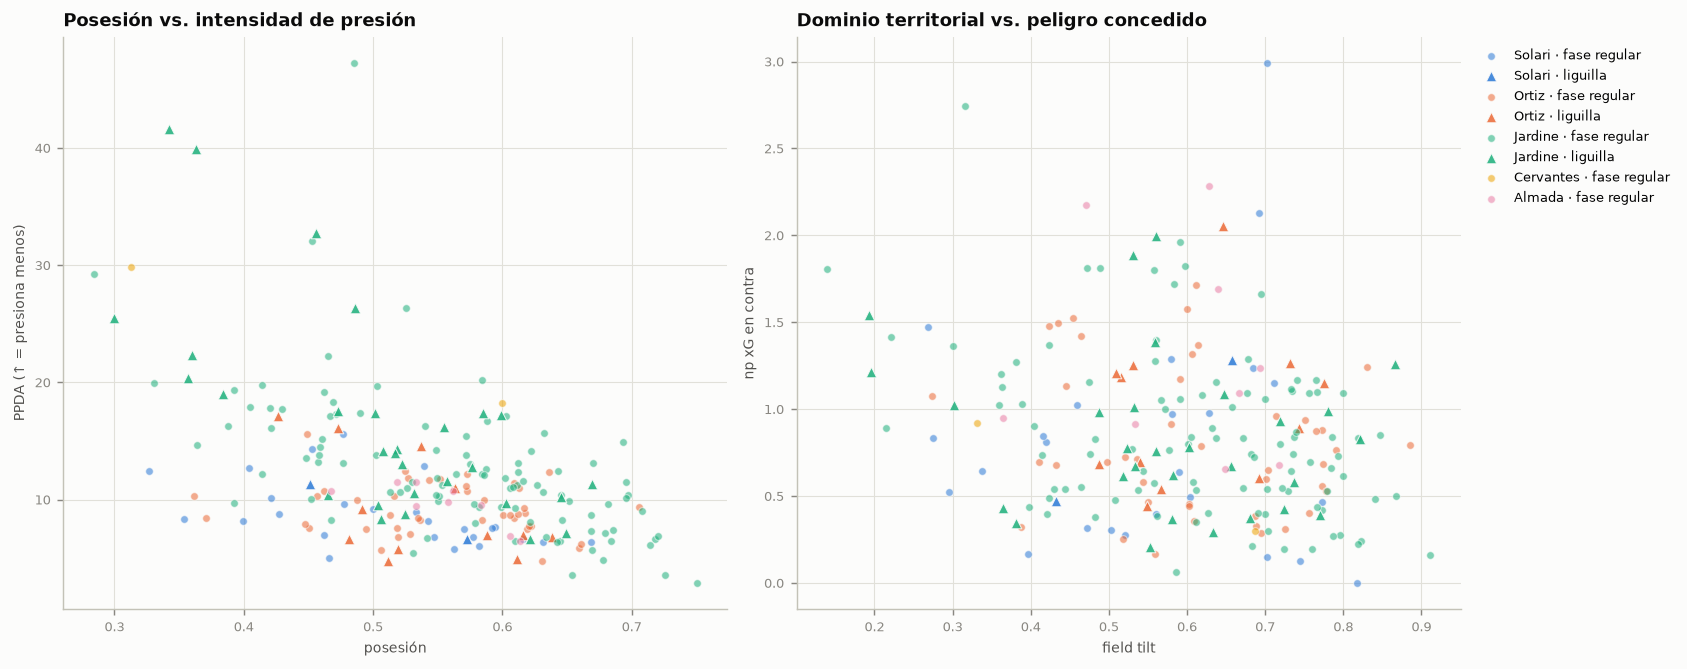
\includegraphics[width=\linewidth]{contexto_plano_estilo}
\caption{Plano de estilo por partido. Izquierda: posesión contra PPDA. Derecha: field tilt contra xG concedido. Los triángulos son partidos de liguilla.}\label{fig:plano}
\end{figure}
El plano de la Figura~\ref{fig:plano} resume la identidad de cada entrenador. Los partidos de Solari y Ortiz se concentran en una franja de PPDA bajo (presión constante) con posesión variable. Los de Jardine se extienden hacia arriba: \textbf{el mismo equipo presiona mucho en unos partidos y casi nada en otros}, y los triángulos de liguilla se ubican en la zona de baja posesión y PPDA alto.

\subsection{Localía}
\begin{table}[H]
\centering
\scriptsize
\caption{Medianas por partido según localía.}
\label{tab:ctx_localia}
\resizebox{\ifdim\width>\linewidth\linewidth\else\width\fi}{!}{%
\begin{tabular}{lrrrrrrrrr}
\toprule
\textbf{Entrenador · localía} & \textbf{Posesión} & \textbf{Field tilt} & \textbf{PPDA} & \textbf{x presión} & \textbf{Pases prog.} & \textbf{Precisión} & \textbf{np xG} & \textbf{np xG c.} & \textbf{n} \\
\midrule
Solari · Local & 0.54 & 0.63 & 6.90 & 60.74 & 26.00 & 0.81 & 0.96 & 0.65 & 14 \\
Solari · Visita & 0.48 & 0.50 & 8.74 & 54.93 & 24.00 & 0.76 & 1.07 & 0.65 & 13 \\
Ortiz · Local & 0.58 & 0.69 & 9.38 & 58.25 & 37.00 & 0.84 & 1.52 & 0.69 & 27 \\
Ortiz · Visita & 0.52 & 0.58 & 7.87 & 56.79 & 35.50 & 0.81 & 1.41 & 0.88 & 28 \\
Jardine · Local & 0.56 & 0.66 & 12.44 & 59.51 & 36.00 & 0.86 & 1.26 & 0.66 & 64 \\
Jardine · Visita & 0.56 & 0.60 & 11.53 & 55.76 & 33.00 & 0.84 & 1.06 & 0.90 & 65 \\
Almada · Local & 0.53 & 0.56 & 11.14 & 54.99 & 43.00 & 0.84 & 1.53 & 1.32 & 4 \\
Almada · Visita & 0.58 & 0.65 & 9.55 & 58.72 & 37.00 & 0.80 & 1.26 & 1.10 & 5 \\
\bottomrule
\end{tabular}}
\end{table}
Con Jardine, de local el equipo inclina más la cancha (field tilt 0.66 contra 0.60 de visita), presiona más arriba ($x$ 59.5 contra 55.8) y concede menos xG (0.66 contra 0.90). Con Ortiz se ve un patrón parecido. La localía, entonces, se asocia con \emph{dónde} se juega más que con cuánto balón se tiene.

\subsection{Nivel del rival}
\begin{table}[H]
\centering
\scriptsize
\caption{Medianas por partido según el nivel del rival (tercil de puntos por partido en la temporada).}
\label{tab:ctx_rival}
\resizebox{\ifdim\width>\linewidth\linewidth\else\width\fi}{!}{%
\begin{tabular}{lrrrrrrrrr}
\toprule
\textbf{Entrenador · rival} & \textbf{Posesión} & \textbf{Field tilt} & \textbf{PPDA} & \textbf{x presión} & \textbf{Pases prog.} & \textbf{Precisión} & \textbf{np xG} & \textbf{np xG c.} & \textbf{n} \\
\midrule
Solari · Alto & 0.48 & 0.52 & 8.92 & 58.19 & 26.00 & 0.76 & 1.11 & 0.65 & 7 \\
Solari · Medio & 0.47 & 0.47 & 8.18 & 57.78 & 22.00 & 0.77 & 0.92 & 0.84 & 11 \\
Solari · Bajo & 0.58 & 0.68 & 7.52 & 60.88 & 30.00 & 0.82 & 1.07 & 0.47 & 9 \\
Ortiz · Alto & 0.54 & 0.55 & 8.43 & 54.83 & 36.00 & 0.83 & 1.32 & 0.94 & 19 \\
Ortiz · Medio & 0.54 & 0.60 & 9.38 & 58.29 & 35.00 & 0.82 & 1.46 & 0.72 & 21 \\
Ortiz · Bajo & 0.57 & 0.61 & 8.67 & 58.25 & 37.00 & 0.83 & 1.83 & 0.72 & 15 \\
Jardine · Alto & 0.51 & 0.56 & 15.21 & 55.85 & 32.50 & 0.84 & 0.93 & 0.83 & 46 \\
Jardine · Medio & 0.57 & 0.64 & 11.36 & 59.69 & 35.00 & 0.85 & 1.17 & 0.74 & 48 \\
Jardine · Bajo & 0.60 & 0.68 & 10.96 & 59.61 & 38.00 & 0.87 & 1.71 & 0.80 & 35 \\
Almada · Alto & 0.58 & 0.59 & 8.80 & 52.13 & 37.00 & 0.81 & 1.28 & 1.30 & 2 \\
Almada · Medio & 0.55 & 0.52 & 10.65 & 51.86 & 41.00 & 0.83 & 1.62 & 1.02 & 2 \\
Almada · Bajo & 0.53 & 0.65 & 9.55 & 58.72 & 44.00 & 0.83 & 1.36 & 1.24 & 5 \\
\bottomrule
\end{tabular}}
\end{table}
\begin{table}[H]
\centering
\small
\caption{Distribución de resultados según nivel del rival (\% de partidos).}
\label{tab:ctx_rival_res}
\resizebox{\ifdim\width>\linewidth\linewidth\else\width\fi}{!}{%
\begin{tabular}{lrrrr}
\toprule
\textbf{Entrenador · rival} & \textbf{\% G} & \textbf{\% E} & \textbf{\% P} & \textbf{n} \\
\midrule
Solari · Alto & 28.60 & 42.90 & 28.60 & 7 \\
Solari · Medio & 45.50 & 36.40 & 18.20 & 11 \\
Solari · Bajo & 44.40 & 22.20 & 33.30 & 9 \\
Ortiz · Alto & 52.60 & 15.80 & 31.60 & 19 \\
Ortiz · Medio & 47.60 & 42.90 & 9.50 & 21 \\
Ortiz · Bajo & 80.00 & 13.30 & 6.70 & 15 \\
Jardine · Alto & 39.10 & 34.80 & 26.10 & 46 \\
Jardine · Medio & 50.00 & 29.20 & 20.80 & 48 \\
Jardine · Bajo & 74.30 & 17.10 & 8.60 & 35 \\
Almada · Alto & 50.00 & 50.00 & 0.00 & 2 \\
Almada · Medio & 50.00 & 0.00 & 50.00 & 2 \\
Almada · Bajo & 80.00 & 20.00 & 0.00 & 5 \\
\bottomrule
\end{tabular}}
\end{table}
\begin{historia}[Lo que se observa]
Con Jardine, contra rivales de nivel \textbf{Alto} el PPDA sube a 15.2 (contra 11.0--11.4 ante rivales Medio y Bajo), la posesión baja a 0.51 (contra 0.60 ante rivales Bajo), el field tilt baja a 0.56 y el np xG propio cae a 0.93. El xG concedido casi no cambia (0.74--0.83). Con Ortiz y Solari el PPDA no cambia con el nivel del rival (8--9). Visto así, Jardine se \emph{adapta} al rival y Ortiz y Solari mantienen un mismo plan.
\end{historia}

\subsection{Fase del torneo: regular contra liguilla}\label{sec:fase}
\begin{table}[H]
\centering
\scriptsize
\caption{Medianas por partido en fase regular y liguilla.}
\label{tab:ctx_fase}
\resizebox{\ifdim\width>\linewidth\linewidth\else\width\fi}{!}{%
\begin{tabular}{lrrrrrrrrr}
\toprule
\textbf{Entrenador · fase} & \textbf{Posesión} & \textbf{Field tilt} & \textbf{PPDA} & \textbf{x presión} & \textbf{Pases prog.} & \textbf{Precisión} & \textbf{np xG} & \textbf{np xG c.} & \textbf{n} \\
\midrule
Solari · Fase regular & 0.53 & 0.58 & 8.18 & 60.14 & 26.00 & 0.79 & 1.07 & 0.65 & 25 \\
Solari · Liguilla & 0.51 & 0.55 & 8.97 & 57.89 & 21.50 & 0.76 & 0.48 & 0.88 & 2 \\
Ortiz · Fase regular & 0.56 & 0.61 & 8.78 & 57.70 & 37.00 & 0.83 & 1.52 & 0.72 & 43 \\
Ortiz · Liguilla & 0.53 & 0.56 & 6.94 & 56.15 & 35.00 & 0.80 & 1.30 & 1.02 & 12 \\
Jardine · Fase regular & 0.58 & 0.63 & 11.56 & 58.59 & 36.00 & 0.86 & 1.19 & 0.80 & 100 \\
Jardine · Liguilla & 0.52 & 0.56 & 14.14 & 56.59 & 29.00 & 0.83 & 1.06 & 0.78 & 29 \\
Almada · Fase regular & 0.56 & 0.64 & 9.76 & 55.90 & 41.00 & 0.83 & 1.36 & 1.10 & 9 \\
\bottomrule
\end{tabular}}
\end{table}
Jardine dirigió 29 partidos de liguilla. En ellos su PPDA sube de 11.6 a 14.1, la posesión baja de 0.58 a 0.52, los pases progresivos bajan de 36 a 29 y la $x$ de presión cae de 58.6 a 56.6. \textbf{El xG concedido no cambia} (0.80 contra 0.78). En la liguilla del Apertura 2024 (cuartos contra Toluca, semifinal contra Cruz Azul y final contra Monterrey) la posesión fue de 30--49\% y el PPDA de 19--42. Ortiz, en cambio, presionó \emph{más} en liguilla (PPDA 6.9).

\subsection{Estado del marcador}
\begin{table}[H]
\centering
\scriptsize
\caption{Comportamiento según el estado del marcador (diferencia de goles antes de cada evento).}
\label{tab:ctx_marcador}
\resizebox{\ifdim\width>\linewidth\linewidth\else\width\fi}{!}{%
\begin{tabular}{lrrrrrrr}
\toprule
\textbf{Entrenador · estado} & \textbf{\% eventos} & \textbf{\% pases AME} & \textbf{x pases} & \textbf{x presiones} & \textbf{\% presión campo rival} & \textbf{xG/100 pases} & \textbf{xG rival/100 pases} \\
\midrule
Solari · Empatando & 63.71 & 51.40 & 55.64 & 60.24 & 49.49 & 0.24 & 0.16 \\
Solari · Ganando & 21.30 & 42.66 & 56.70 & 55.78 & 43.32 & 0.40 & 0.27 \\
Solari · Perdiendo & 14.99 & 60.81 & 61.12 & 58.20 & 48.01 & 0.28 & 0.46 \\
Ortiz · Empatando & 43.38 & 56.39 & 60.93 & 59.44 & 49.72 & 0.29 & 0.24 \\
Ortiz · Ganando & 37.93 & 50.40 & 58.33 & 54.73 & 41.24 & 0.43 & 0.24 \\
Ortiz · Perdiendo & 18.69 & 61.92 & 64.55 & 57.41 & 46.31 & 0.33 & 0.23 \\
Jardine · Empatando & 53.99 & 55.17 & 58.54 & 58.72 & 48.18 & 0.26 & 0.19 \\
Jardine · Ganando & 31.02 & 50.43 & 56.21 & 53.89 & 39.95 & 0.35 & 0.22 \\
Jardine · Perdiendo & 14.99 & 63.29 & 63.45 & 61.96 & 53.27 & 0.32 & 0.26 \\
Almada · Empatando & 41.24 & 57.87 & 60.21 & 58.51 & 48.21 & 0.30 & 0.40 \\
Almada · Ganando & 44.25 & 50.52 & 57.77 & 54.11 & 41.50 & 0.31 & 0.29 \\
Almada · Perdiendo & 14.51 & 60.10 & 68.70 & 55.63 & 44.64 & 0.75 & 0.51 \\
\bottomrule
\end{tabular}}
\end{table}
Con todos los entrenadores se repite la misma dinámica: \textbf{cuando va ganando, el América cede el balón} (alrededor del 50\% de los pases del partido) y baja la altura de sus presiones. \textbf{Cuando va perdiendo}, sube la posesión (60--63\%) y adelanta la presión. Con Jardine la reacción es la más marcada: el 53\% de sus presiones son en campo rival cuando pierde, contra 40\% cuando gana. Con Jardine el América pasa el 54\% del tiempo (en eventos) empatado, el 31\% ganando y el 15\% perdiendo.

\subsection{Balón parado}
\begin{table}[H]
\centering
\scriptsize
\caption{Origen del xG (\% del total) por patrón de juego: América y sus rivales.}
\label{tab:ctx_bp}
\resizebox{\ifdim\width>\linewidth\linewidth\else\width\fi}{!}{%
\begin{tabular}{lrrrrrrrr}
\toprule
\textbf{Lado · entrenador} & \textbf{Juego abierto} & \textbf{Counter} & \textbf{Corner} & \textbf{Free Kick} & \textbf{Throw In} & \textbf{Goal Kick} & \textbf{Keeper} & \textbf{Kick Off} \\
\midrule
América · Almada & 49.1 & 7.7 & 20.2 & 9.2 & 8.6 & 1.6 & 2.6 & 0.9 \\
América · Jardine & 52.3 & 2.4 & 12.7 & 15.7 & 10.9 & 3.3 & 1.9 & 0.7 \\
América · Ortiz & 50.4 & 3.0 & 11.8 & 14.4 & 12.5 & 4.7 & 2.1 & 1.1 \\
América · Solari & 53.1 & 0.1 & 15.5 & 16.8 & 9.8 & 2.4 & 1.0 & 1.4 \\
Rival · Almada & 47.5 & 0.2 & 14.6 & 4.2 & 21.4 & 5.6 & 6.4 & 0.2 \\
Rival · Jardine & 43.9 & 2.8 & 18.4 & 12.3 & 14.6 & 5.4 & 1.6 & 1.1 \\
Rival · Ortiz & 50.8 & 2.3 & 14.9 & 14.4 & 9.9 & 5.4 & 1.4 & 0.9 \\
Rival · Solari & 55.8 & 0.9 & 12.0 & 19.8 & 8.1 & 3.1 & 0.1 & 0.1 \\
\bottomrule
\end{tabular}}
\end{table}
Con Jardine, cerca del \textbf{39\% del xG del América viene de reanudaciones}: tiro libre 15.7\%, córner 12.7\% y saque de banda 10.9\%. Su contragolpe aporta poco (2.4\%). Los rivales de Jardine obtienen el 18.4\% de su xG en córners, la proporción más alta entre los entrenadores. Esto apunta a una posible zona vulnerable en defensa de córners. Con Almada el contragolpe sube a 7.7\% del xG.

\subsection{Sustituciones y cambios de sistema}
\begin{table}[H]
\centering
\scriptsize
\caption{Sustituciones del América por entrenador.}
\label{tab:ctx_subs}
\resizebox{\ifdim\width>\linewidth\linewidth\else\width\fi}{!}{%
\begin{tabular}{lrrrrrrrr}
\toprule
\textbf{Entrenador} & \textbf{Cambios} & \textbf{Min. mediano} & \textbf{\% al descanso} & \textbf{Por partido} & \textbf{1.er cambio (min)} & \textbf{\% empatando} & \textbf{\% ganando} & \textbf{\% perdiendo} \\
\midrule
Solari & 111 & 68.00 & 5.41 & 4.11 & 57 & 45.00 & 30.60 & 24.30 \\
Ortiz & 251 & 73.00 & 3.98 & 4.56 & 62 & 25.10 & 55.40 & 19.50 \\
Jardine & 603 & 73.00 & 10.12 & 4.67 & 59 & 33.20 & 44.60 & 22.20 \\
Almada & 42 & 72.50 & 9.52 & 4.67 & 61 & 16.70 & 64.30 & 19.00 \\
\bottomrule
\end{tabular}}
\end{table}
\begin{table}[H]
\centering
\small
\caption{Cambios tácticos en vivo (evento \texttt{Tactical Shift}) del América.}
\label{tab:ctx_tacticos}
\resizebox{\ifdim\width>\linewidth\linewidth\else\width\fi}{!}{%
\begin{tabular}{lrrrr}
\toprule
\textbf{Entrenador} & \textbf{Por partido} & \textbf{\% empatando} & \textbf{\% ganando} & \textbf{\% perdiendo} \\
\midrule
Solari & 0.81 & 36.40 & 27.30 & 36.40 \\
Ortiz & 0.85 & 25.50 & 48.90 & 25.50 \\
Jardine & 1.80 & 38.40 & 38.40 & 23.30 \\
Almada & 1.78 & 18.80 & 56.20 & 25.00 \\
\bottomrule
\end{tabular}}
\end{table}
Todos los entrenadores hacen alrededor de 4.5 cambios por partido, y el primero hacia el minuto 57--62. Las diferencias están en \emph{cómo} intervienen:
\begin{itemize}
  \item Jardine hace el \textbf{10\% de sus cambios al medio tiempo} (Ortiz, 4\%).
  \item Jardine registra \textbf{1.8 cambios tácticos en vivo por partido}, más del doble que Solari y Ortiz (0.8).
  \item Ortiz y Almada concentran sus cambios cuando van ganando (55\% y 64\%). Los de Jardine se reparten más entre los tres estados del marcador.
\end{itemize}

% =====================================================================
\section{La historia que cuentan los datos}\label{sec:historia}
% =====================================================================
Juntando las piezas, los datos esbozan un relato. Por ahora es una \textbf{hipótesis}, no una conclusión.

\begin{historia}[Un relato en cinco actos (a validar)]
\textbf{1. La identidad del club no está en la posesión.} Con los cinco entrenadores el América tiene alrededor del 55\% del balón. Lo que cambia es la \emph{calidad} de esa posesión y la \emph{forma de defender}.

\textbf{2. De Solari a Ortiz: el equipo aprende a progresar.} La precisión sube (0.79 $\to$ 0.83) y los pases progresivos también (26 $\to$ 36), con una presión intensa y constante (PPDA de 8 a 9).

\textbf{3. Jardine: control con balón y presión a la carta.} Tiene la precisión más alta del periodo (0.85) y el PPDA más alto y variable (12.2, IQR 9.6--16.4). Presiona arriba contra rivales débiles y cuando va perdiendo; ante rivales fuertes, en liguilla o con ventaja se repliega y cede el balón, sin conceder más xG. Hace ajustes en vivo (1.8 cambios tácticos por partido, 9 formaciones) y depende del balón parado (39\% de su xG).

\textbf{4. Desgaste o evolución en la etapa de Jardine.} Con los torneos el field tilt sube, pero el xG propio y el porcentaje de victorias bajan (Clausura 2026: 37\%). El dominio territorial ya no se traduce en ocasiones.

\textbf{5. Almada: ¿un giro de estilo?} Sale más corto desde el portero, defiende con la línea más alta y presiona de forma más constante, pero concede más. Con solo 9 partidos es un epílogo, no un capítulo.
\end{historia}

\subsection{Hipótesis para la fase de análisis}
El entregable del hackathon es una \textbf{metodología que permita al club entender el estilo de un entrenador y las
características que lo definen}, evaluada por su análisis estratégico, su justificación con datos, su valor para el
club (ROI y activación) y su escalabilidad. Las hipótesis se reformulan con ese fin: cada una dice qué se espera
encontrar, qué evidencia descriptiva la sugiere, cómo se contrastará y \emph{para qué le sirve al club}. Todas se
contrastan con la \textbf{partición oficial}: la ventana del hackathon (Apertura 2021 -- Clausura 2025) para construir
y los partidos de 2025--2026 para validar y probar.

{\small
\begin{longtable}{p{0.55cm}p{4.4cm}p{3.6cm}p{3.6cm}p{3.2cm}}
\caption{Hipótesis orientadas al resultado del hackathon. Entre paréntesis, el componente del reto (5.1 estilo, 5.2 consistencia y contexto, 5.3 jugadores, 5.4 balón parado, 5.5 evidencia) y el criterio de evaluación.}\label{tab:hipotesis}\\
\toprule \textbf{H} & \textbf{Hipótesis} & \textbf{Evidencia del EDA} & \textbf{Cómo contrastarla} & \textbf{Valor para el club}\\\midrule\endfirsthead
\toprule \textbf{H} & \textbf{Hipótesis} & \textbf{Evidencia del EDA} & \textbf{Cómo contrastarla} & \textbf{Valor para el club}\\\midrule\endhead
\bottomrule\endfoot
H1 & \textbf{Cada entrenador tiene un ADN distinguible}: su perfil de juego lo separa de la liga y de los otros técnicos del América (5.1; análisis estratégico). & La posesión no los separa (0.53--0.56), pero el PPDA, la precisión y la progresión sí (Tabla~\ref{tab:ctx_coach}). & Perfil de 8 ejes frente a la liga ajustado por rival y localía; clasificador ``¿qué técnico dirigió este partido?''. & Describir a cualquier técnico con el mismo lenguaje y en un solo gráfico.\\
H2 & \textbf{Identidad del club frente a identidad del técnico}: algunos rasgos se mantienen con todos (control del balón) y otros cambian con el técnico (presión) (5.2; estratégico). & Posesión estable entre técnicos; PPDA de 8.2 a 12.2 (Figura~\ref{fig:box}). & Varianza de cada eje entre técnicos frente a dentro del técnico, sobre el perfil ajustado. & Saber qué exigir a cualquier técnico (lo innegociable) y qué depende de su idea.\\
H3 & \textbf{Jardine adapta su plan al rival} más que Solari y Ortiz (5.2 contexto). & PPDA 15.2 contra rivales fuertes y 11 contra el resto; sin cambio con Ortiz (Tabla~\ref{tab:ctx_rival}). & Perfil por tercil de fuerza del rival (previa, sin leakage) con intervalos bootstrap. & Anticipar cómo jugará el equipo según el rival.\\
H4 & \textbf{El marcador cambia el plan}: ganando se cede el balón y perdiendo se presiona arriba; en Jardine el ajuste es mayor (5.2). & Tabla~\ref{tab:ctx_marcador}. & Modelo por tramo y estado del marcador (T2). & Leer las decisiones en vivo del técnico.\\
H5 & \textbf{En liguilla el equipo se vuelve reactivo sin conceder más} (5.2). & PPDA 14.1 contra 11.6; posesión 0.52 contra 0.58; mismo xG concedido (Tabla~\ref{tab:ctx_fase}). & Perfil por fase (regular o liguilla). & Planear el cierre de torneo.\\
H6 & \textbf{El dominio territorial dejó de convertirse en ocasiones} al final de la etapa de Jardine (5.2 evolución). & Field tilt de 0.61 a 0.68 y np xG de 1.34 a 1.04 (Tabla~\ref{tab:ctx_torneo}). & Evolución del ADN por torneo, validada con 2025--2026 (datos no vistos). & Señal temprana de desgaste de un proyecto.\\
H7 & \textbf{El juego se construye desde atrás y está repartido}: ningún jugador lo sostiene solo (5.3). & 10 de los 15 jugadores con más minutos tienen un OBV/90 de 0.18 a 0.31; ninguno se despega (Tabla~\ref{tab:player_min}). & Gini y reparto del OBV por línea; roles de jugador. & Saber qué perfiles necesita el sistema de cada técnico.\\
H8 & \textbf{El balón parado es pilar ofensivo y punto débil defensivo} (5.4). & 39\% del xG propio de reanudaciones y 18.4\% del xG rival de córners (Tabla~\ref{tab:ctx_bp}). & Eje de balón parado del ADN frente a la liga; mapas de entrega y remate. & Priorizar entrenamiento específico.\\
H9 & \textbf{La metodología detecta un cambio de entrenador que nunca vio}: los partidos de Almada en 2026 salen del ADN de Jardine y se parecen a su propio ADN en Pachuca (5.5; escalabilidad). & El EDA ya muestra a Almada distinto (línea más alta, salida corta), con 9 partidos. & Distancia al ADN de Jardine en validación y prueba; clasificador entrenado con toda la liga en la ventana oficial. & Monitorear si un técnico mantiene su identidad y evaluar a un técnico por su historial en otro club.\\
H10 & \textbf{Un Índice de Encaje ordena a los técnicos de la liga por parecido con la identidad del América} (negocio; ROI). & Los técnicos del América difieren en presión y precisión, no en posesión (H1, H2). & Distancia del ADN de cada técnico de la liga al ADN histórico del club. & Reducir el riesgo de una contratación fallida (ROI) y dar una lista corta de candidatos.\\
\end{longtable}}

% =====================================================================
\section{Implicaciones para el marco analítico}\label{sec:marco}
% =====================================================================
El reto exige definir los objetos antes del análisis. Con base en lo observado se proponen las siguientes definiciones preliminares:
\begin{itemize}
  \item \textbf{Posesión}: la \col{possession} de StatsBomb (cambia cuando el rival toma el control del balón). Es consistente y está disponible en todos los eventos.
  \item \textbf{Secuencia ofensiva}: una posesión del América con 3 pases o más (la mediana), o que llega al último tercio.
  \item \textbf{Construcción}: una posesión que inicia en $x<40$ desde saque de meta, del portero o en juego abierto. La salida corta o larga del portero se toma de \col{gk_long_pass_ratio}.
  \item \textbf{Transición}: los eventos con \col{is_transition}, validados contra una definición propia: recuperación y llegada al último tercio en 15 segundos o menos.
  \item \textbf{Fase de presión}: las acciones defensivas del América con $x\geq60$. La intensidad se mide con el PPDA y la reacción tras pérdida con \col{counterpress}.
  \item \textbf{Contexto}: estado del marcador antes del evento, minuto (tramos de 15), localía, nivel del rival (tercil de puntos por partido) y fase (regular o liguilla).
  \item \textbf{Métricas}: una por familia (Tabla~\ref{tab:team_top_corr}). Se usan medianas, métricas por 90 minutos y tasas por posesión; OBV mide el dominio y xG la ocasión.
\end{itemize}

\paragraph{Supuestos explícitos.} (i) El nivel del rival se mide con puntos por partido en toda la temporada, que incluye el propio partido contra el América. (ii) El 360 solo describe a los jugadores visibles. (iii) La ``temporada'' mezcla dos torneos y liguillas, por lo que las comparaciones temporales se hacen por torneo. (iv) El número de eventos se usa como aproximación del tiempo en cada estado del marcador.

\paragraph{Alcance y límites.} El marco describe patrones de equipo a partir de eventos. No observa lo que ocurre sin balón fuera de cámara, instrucciones del entrenador, lesiones ni calendario, y sus comparaciones son asociaciones, no causas.

% =====================================================================
\section{Limitaciones de este EDA}
% =====================================================================
\begin{itemize}
  \item \textbf{Todo es descriptivo}: no hay pruebas de hipótesis ni intervalos de confianza, y las diferencias no se ajustaron por rival, calendario o plantilla.
  \item \textbf{Muestras desbalanceadas}: Jardine tiene 129 partidos, Solari 27, Almada 9 y Cervantes 2. Las comparaciones con Almada son indicativas.
  \item \textbf{Confusión entre entrenador y contexto}: cada entrenador tuvo plantillas y rivales distintos. Con los datos disponibles no se puede separar el efecto del entrenador del de los jugadores.
  \item \textbf{Definiciones preliminares}: el pase progresivo, el field tilt y el nivel del rival pueden cambiar en el marco analítico final.
  \item \textbf{360 parcial} y análisis 360 hecho sobre una muestra de 20 partidos.
\end{itemize}

% =====================================================================
\section{Siguientes pasos}
% =====================================================================
\begin{enumerate}
  \item Construir el \textbf{ADN del entrenador}: un perfil de 8 ejes de juego para cualquier técnico de la Liga MX,
        comparado con toda la liga y ajustado por rival y localía (H1, H2, H10).
  \item Usar la \textbf{partición oficial}: la ventana del hackathon para construir; 2025--2026 para validar y probar,
        incluido el cambio a Almada (H9).
  \item Formalizar el marco analítico y contrastar H3--H8 con modelos que controlen por rival y localía.
  \item Traducir los resultados al \textbf{valor para el club}: contratación y seguimiento de técnicos, preparación de
        partidos y un ROI con escenarios.
  \item Entregar en el formato oficial: un \textbf{reporte HTML} interactivo y un video de 5 minutos.
\end{enumerate}

\appendix
% =====================================================================
\section{Diccionario de datos}\label{app:dic}
% =====================================================================
{\scriptsize
\begin{longtable}{p{4.3cm}p{2.2cm}p{8.8cm}}
\caption{Diccionario de columnas de eventos.}\label{tab:dic_eventos}\\
\toprule
\textbf{Columna} & \textbf{Aplica a} & \textbf{Significado} \\
\midrule
\endfirsthead
\toprule
\textbf{Columna} & \textbf{Aplica a} & \textbf{Significado} \\
\midrule
\endhead
\bottomrule
\endfoot
id & Todos & Identificador único (UUID) del evento. \\
index & Todos & Orden secuencial del evento dentro del partido (1, 2, 3...). \\
match\_id & Todos & Identificador del partido. \\
period & Todos & Periodo: 1 y 2 = tiempos regulares; 3 y 4 = tiempos extra; 5 = tanda de penales. \\
timestamp & Todos & Tiempo dentro del periodo (hh:mm:ss.mmm). \\
minute & Todos & Minuto de juego acumulado (el 2.º tiempo inicia en 45). \\
second & Todos & Segundo dentro del minuto (0-59). \\
duration & Todos & Duración del evento en segundos (p. ej. tiempo de vuelo de un pase o de una conducción). \\
type & Todos & Tipo de evento (Pass, Carry, Pressure, Shot, Duel, ...). Define qué columnas específicas tienen valor. \\
team & Todos & Equipo que ejecuta el evento. \\
team\_id & Todos & Identificador del equipo que ejecuta el evento. \\
player & Todos & Jugador que ejecuta el evento. \\
player\_id & Todos & Identificador del jugador. \\
position & Todos & Posición táctica del jugador en ese momento (según la formación vigente). \\
possession & Todos & Número secuencial de posesión en el partido; cambia cuando el otro equipo toma control del balón. \\
possession\_team & Todos & Equipo que tiene la posesión (puede diferir de team: p. ej. una presión del rival). \\
possession\_team\_id & Todos & Identificador del equipo en posesión. \\
play\_pattern & Todos & Cómo inició la posesión: Regular Play, From Throw In, From Free Kick, From Corner, From Goal Kick, From Counter, From Keeper, From Kick Off, Other. \\
is\_controlled\_possession & Todos & Flag StatsBomb: el evento ocurre en una posesión controlada (juego elaborado). \\
is\_transition & Todos & Flag StatsBomb: el evento ocurre en una fase de transición (posesión recién ganada y rápida). \\
possession\_directness & Todos & Qué tan directa es la posesión hacia la portería rival (avance vertical relativo al recorrido total). \\
player\_possession\_directness & Todos & Directness de la contribución del jugador dentro de la posesión. \\
set\_piece\_phase & Todos & Fase de la jugada a balón parado: 1 = primer contacto tras el saque, 2 = segunda jugada. \\
under\_pressure & Todos & Flag: el ejecutor estaba siendo presionado por un rival (NaN = no). \\
counterpress & Todos & Flag: acción de presión/defensa dentro de los 5 s posteriores a una pérdida propia (NaN = no). \\
off\_camera & Todos & Flag: el evento ocurrió fuera de cámara (ubicación estimada). \\
out & Todos & Flag: la acción terminó con el balón fuera del campo. \\
related\_events & Todos & Lista de ids de eventos relacionados (p. ej. un pase y su recepción). \\
tactics & Starting XI / Tactical Shift & Formación y lista de jugadores con posición (JSON). \\
attacking\_direction & Todos & Dirección de ataque del equipo en la toma original (left\_to\_right / right\_to\_left). Las coordenadas ya vienen normalizadas. \\
location & Todos & Coordenadas [x, y] del evento en la cancha 120 x 80 (x hacia la portería rival). \\
location\_x & Todos & Coordenada x derivada de location (0 = propia portería, 120 = portería rival). \\
location\_y & Todos & Coordenada y derivada de location (0 a 80, de banda a banda). \\
location\_bucket & Todos & Tercio del campo: defensive\_third, midfield\_third, final\_third. \\
control\_degree & Todos & Grado de control del balón en la acción (0 a 1). \\
obv\_for\_before & Acciones con balón & Probabilidad (modelo OBV) de que el equipo en posesión marque antes de la acción. \\
obv\_for\_after & Acciones con balón & Probabilidad de marcar después de la acción. \\
obv\_for\_net & Acciones con balón & Cambio en la probabilidad de marcar causado por la acción (after - before). \\
obv\_against\_before & Acciones con balón & Probabilidad de recibir gol antes de la acción. \\
obv\_against\_after & Acciones con balón & Probabilidad de recibir gol después de la acción. \\
obv\_against\_net & Acciones con balón & Cambio en la probabilidad de recibir gol. \\
obv\_total\_net & Acciones con balón & On-Ball Value neto: obv\_for\_net - obv\_against\_net. Valor total de la acción. \\
pass\_length & Pass & Longitud del pase (yardas). \\
pass\_angle & Pass & Ángulo del pase en radianes (0 = hacia adelante, +/-pi = hacia atrás). \\
pass\_end\_location & Pass & Coordenadas [x, y] donde termina el pase. \\
pass\_height & Pass & Altura: Ground Pass, Low Pass (bajo la cintura), High Pass (sobre la cabeza). \\
pass\_body\_part & Pass & Parte del cuerpo: Right Foot, Left Foot, Head, Keeper Arm, ... \\
pass\_type & Pass & Tipo de pase especial: Recovery, Throw-in, Free Kick, Goal Kick, Corner, Interception, Kick Off. Nulo = pase regular en juego abierto. \\
pass\_outcome & Pass & Resultado: Incomplete, Out, Pass Offside, Unknown, Injury Clearance. Nulo = pase completo. \\
pass\_technique & Pass & Técnica: Inswinging, Outswinging, Straight, Through Ball. \\
pass\_recipient & Pass & Jugador que recibe el pase. \\
pass\_recipient\_id & Pass & Identificador del receptor. \\
pass\_cross & Pass & Flag: centro. \\
pass\_switch & Pass & Flag: cambio de orientación (cruza gran parte del ancho del campo). \\
pass\_through\_ball & Pass & Flag: pase filtrado entre líneas defensivas. \\
pass\_cut\_back & Pass & Flag: pase atrás desde línea de fondo. \\
pass\_shot\_assist & Pass & Flag: el pase precede a un tiro (pase clave). \\
pass\_goal\_assist & Pass & Flag: el pase precede a un gol (asistencia). \\
pass\_assisted\_shot\_id & Pass & Id del tiro que generó el pase. \\
pass\_aerial\_won & Pass & Flag: pase ejecutado tras ganar un duelo aéreo. \\
pass\_deflected & Pass & Flag: pase desviado. \\
pass\_miscommunication & Pass & Flag: pase fallido por mala comunicación. \\
pass\_no\_touch & Pass & Flag: pase dejado pasar sin tocar (dummy). \\
pass\_inswinging & Pass & Flag: centro/córner cerrado hacia portería. \\
pass\_outswinging & Pass & Flag: centro/córner abierto. \\
pass\_straight & Pass & Flag: centro/córner recto. \\
pass\_backheel & Pass & Flag: pase de tacón. \\
pass\_pass\_success\_probability & Pass & Probabilidad modelada (StatsBomb) de que el pase se complete. \\
pass\_pass\_cluster\_id & Pass & Clúster de pase (familia de pases con origen/destino/dirección similares). \\
pass\_pass\_cluster\_label & Pass & Etiqueta legible del clúster (tercio, carril y dirección). \\
pass\_pass\_cluster\_probability & Pass & Probabilidad de pertenencia del pase a su clúster. \\
pass\_xclaim & Pass & Probabilidad de que el portero rival intercepte un centro. \\
pass\_duel\_win\_probability & Pass & Probabilidad de ganar el duelo asociado al pase. \\
shot\_statsbomb\_xg & Shot & Goles esperados (xG) del tiro: probabilidad de gol antes del disparo. \\
shot\_shot\_execution\_xg & Shot & xG post-disparo: probabilidad de gol considerando la ejecución (dirección, potencia). \\
shot\_shot\_execution\_xg\_uplift & Shot & Diferencia entre xG de ejecución y xG previo: calidad de la definición. \\
shot\_gk\_save\_difficulty\_xg & Shot & Dificultad de atajada para el portero (tiros a puerta). \\
shot\_gk\_positioning\_xg\_suppression & Shot & xG suprimido por el posicionamiento del portero. \\
shot\_gk\_shot\_stopping\_xg\_suppression & Shot & xG suprimido por la atajada del portero. \\
shot\_outcome & Shot & Resultado: Goal, Saved, Off T, Blocked, Wayward, Post, Saved to Post, Saved Off Target. \\
shot\_type & Shot & Tipo: Open Play, Free Kick, Penalty. \\
shot\_body\_part & Shot & Parte del cuerpo con la que se remata. \\
shot\_technique & Shot & Técnica: Normal, Half Volley, Volley, Lob, Overhead Kick, Diving Header, Backheel. \\
shot\_end\_location & Shot & Coordenadas [x, y, z] donde termina el tiro. \\
shot\_freeze\_frame & Shot & Posición de todos los jugadores en el momento del tiro (JSON). \\
shot\_key\_pass\_id & Shot & Id del pase que generó el tiro. \\
shot\_first\_time & Shot & Flag: remate de primera. \\
shot\_one\_on\_one & Shot & Flag: mano a mano con el portero. \\
shot\_deflected & Shot & Flag: tiro desviado. \\
shot\_aerial\_won & Shot & Flag: remate tras ganar duelo aéreo. \\
shot\_follows\_dribble & Shot & Flag: tiro inmediatamente después de un regate. \\
shot\_open\_goal & Shot & Flag: tiro a portería vacía. \\
shot\_redirect & Shot & Flag: desvío de un tiro de compañero. \\
shot\_saved\_to\_post & Shot & Flag: atajado y pega en el poste. \\
shot\_saved\_off\_target & Shot & Flag: atajado aunque iba fuera. \\
shot\_duel\_win\_probability & Shot & Probabilidad de ganar el duelo asociado al tiro. \\
shot\_shot\_shot\_assist & Shot & Flag: el tiro (rebote) asiste otro tiro. \\
shot\_shot\_goal\_assist & Shot & Flag: el tiro (rebote) asiste un gol. \\
carry\_end\_location & Carry & Coordenadas [x, y] donde termina la conducción. \\
dribble\_outcome & Dribble & Resultado del regate: Complete / Incomplete. \\
dribble\_nutmeg & Dribble & Flag: caño. \\
dribble\_overrun & Dribble & Flag: el jugador se pasa del balón. \\
dribble\_no\_touch & Dribble & Flag: regate sin tocar el balón (amague). \\
ball\_receipt\_outcome & Ball Receipt* & Resultado de la recepción: nulo = correcta; Incomplete = fallida. \\
miscontrol\_aerial\_won & Miscontrol & Flag: mal control tras duelo aéreo ganado. \\
miscontrol\_duel\_win\_probability & Miscontrol & Probabilidad de ganar el duelo asociado. \\
duel\_type & Duel & Tipo de duelo: Tackle (entrada) o Aerial Lost. \\
duel\_outcome & Duel & Resultado: Won, Success In Play, Success Out, Lost In Play, Lost Out. \\
duel\_duel\_win\_probability & Duel & Probabilidad modelada de ganar el duelo. \\
duel\_hops\_rating & Duel & Rating HOPS (habilidad aérea) del jugador. \\
duel\_hops\_raw\_rating & Duel & Rating HOPS sin ajustar del jugador. \\
duel\_hops\_opponent\_rating & Duel & Rating HOPS del oponente en el duelo. \\
duel\_hops\_opponent\_raw\_rating & Duel & Rating HOPS sin ajustar del oponente. \\
interception\_outcome & Interception & Resultado: Won, Success In Play, Lost In Play, Lost Out, Success Out. \\
clearance\_body\_part & Clearance & Parte del cuerpo del despeje. \\
clearance\_head & Clearance & Flag: despeje de cabeza. \\
clearance\_left\_foot & Clearance & Flag: despeje con pie izquierdo. \\
clearance\_right\_foot & Clearance & Flag: despeje con pie derecho. \\
clearance\_other & Clearance & Flag: despeje con otra parte del cuerpo. \\
clearance\_aerial\_won & Clearance & Flag: despeje tras ganar duelo aéreo. \\
clearance\_duel\_win\_probability & Clearance & Probabilidad de ganar el duelo asociado al despeje. \\
block\_deflection & Block & Flag: el bloqueo desvía el balón. \\
block\_offensive & Block & Flag: bloqueo de un compañero (ofensivo). \\
block\_save\_block & Block & Flag: bloqueo que evita un gol en la línea. \\
ball\_recovery\_offensive & Ball Recovery & Flag: recuperación en fase ofensiva. \\
ball\_recovery\_recovery\_failure & Ball Recovery & Flag: intento de recuperación fallido. \\
50\_50 & 50/50 & Balón dividido: resultado (JSON). \\
defensive\_responsibility & Varios & Jugadores con responsabilidad defensiva en la acción (JSON). \\
foul\_committed\_type & Foul Committed & Tipo de falta: Handball, Dangerous Play, Dive, 6 Seconds, Foul Out. \\
foul\_committed\_card & Foul Committed & Tarjeta: Yellow Card, Second Yellow, Red Card. \\
foul\_committed\_advantage & Foul Committed & Flag: se aplicó ley de la ventaja. \\
foul\_committed\_offensive & Foul Committed & Flag: falta ofensiva. \\
foul\_committed\_penalty & Foul Committed & Flag: falta que resulta en penal. \\
foul\_won\_advantage & Foul Won & Flag: falta recibida con ventaja. \\
foul\_won\_defensive & Foul Won & Flag: falta recibida en acción defensiva. \\
foul\_won\_penalty & Foul Won & Flag: penal recibido. \\
bad\_behaviour\_card & Bad Behaviour & Tarjeta por conducta (fuera de una falta). \\
goalkeeper\_type & Goal Keeper & Acción del portero: Shot Faced, Shot Saved, Goal Conceded, Keeper Sweeper, Punch, Collected, ... \\
goalkeeper\_outcome & Goal Keeper & Resultado de la acción del portero: Success, No Touch, Claim, In Play Safe, Touched Out, ... \\
goalkeeper\_technique & Goal Keeper & Técnica: Standing, Diving. \\
goalkeeper\_position & Goal Keeper & Posición del portero: Set, Moving, Prone. \\
goalkeeper\_body\_part & Goal Keeper & Parte del cuerpo usada por el portero. \\
goalkeeper\_end\_location & Goal Keeper & Coordenadas donde termina la acción del portero. \\
goalkeeper\_punched\_out & Goal Keeper & Flag: despeje de puños. \\
goalkeeper\_shot\_saved\_to\_post & Goal Keeper & Flag: atajada que pega en el poste. \\
goalkeeper\_shot\_saved\_off\_target & Goal Keeper & Flag: atajada de tiro que iba fuera. \\
goalkeeper\_success\_in\_play & Goal Keeper & Flag: acción exitosa con balón en juego. \\
goalkeeper\_lost\_out & Goal Keeper & Flag: acción perdida con balón fuera. \\
substitution\_outcome & Substitution & Razón del cambio: Tactical, Injury, ... \\
substitution\_outcome\_id & Substitution & Id de la razón del cambio. \\
substitution\_replacement & Substitution & Jugador que entra. \\
substitution\_replacement\_id & Substitution & Id del jugador que entra. \\
injury\_stoppage\_in\_chain & Injury Stoppage & Flag: pausa por lesión dentro de una cadena de juego. \\
half\_start\_late\_video\_start & Half Start & Flag: el video del periodo empezó tarde. \\
player\_off\_permanent & Player Off & Flag: el jugador sale de forma permanente. \\
match\_date & Contexto & Fecha del partido (agregada desde matches). \\
season & Contexto & Temporada StatsBomb (Apertura + Clausura). \\
match\_week & Contexto & Jornada. \\
team\_manager & Contexto & Entrenador del América en ese partido. \\
opponent & Contexto & Rival del América. \\
is\_home & Contexto & True si el América juega de local. \\
goals\_for & Contexto & Goles del América en el partido (marcador final). \\
goals\_against & Contexto & Goles recibidos por el América (marcador final). \\
result & Contexto & Resultado del América: W / D / L. \\
\end{longtable}
}
{\scriptsize
\begin{longtable}{p{4.3cm}p{11.2cm}}
\caption{Familias de métricas agregadas (\texttt{team\_match\_*} y \texttt{player\_match\_*}).}\label{tab:dic_familias}\\
\toprule
\textbf{Familia / prefijo} & \textbf{Significado} \\
\midrule
\endfirsthead
\toprule
\textbf{Familia / prefijo} & \textbf{Significado} \\
\midrule
\endhead
\bottomrule
\endfoot
np\_ & Non-penalty: excluye penales (np\_xg, np\_shots, np\_gd...). \\
op\_ & Open play: solo jugadas en juego abierto (op\_xg, op\_shots, op\_passes...). \\
sp\_ & Set piece: jugadas a balón parado (sp\_xg, sp\_goals, sp\_shot\_ratio...). \\
*\_conceded & La misma métrica pero del rival contra el América (np\_xg\_conceded, obv\_conceded...). \\
xg, xgd & Goles esperados y su diferencia (a favor - en contra). \\
possession & Proporción del tiempo de posesión del equipo (0-1). \\
ppda & Pases del rival permitidos por acción defensiva en su propia zona de salida. Más alto = presión menos intensa. \\
defensive\_distance & Distancia media (yardas) desde la propia portería a la que el equipo hace sus acciones defensivas: altura del bloque. \\
directness & Qué tan directas son las posesiones (avance vertical / recorrido). \\
pace\_towards\_goal & Velocidad de avance hacia la portería rival (yardas/segundo). \\
gk\_long\_pass\_ratio, gk\_pass\_distance & Proporción de pases largos del portero y distancia media: tipo de salida desde atrás. \\
passing\_ratio & ANOMALÍA: en esta API coincide con opp\_final\_third\_pass\_ratio; no usar como precisión de pase. \\
successful\_passes / passes & Precisión de pase real (pass\_completion, calculada en el proyecto). \\
deep\_progressions & Pases, conducciones o regates que entran al último tercio. \\
deep\_completions & Pases completados a menos de 20 m de la portería rival. \\
box\_cross\_ratio, crosses\_into\_box & Proporción de pases al área que son centros; centros al área. \\
pressures, counterpressures & Presiones y contrapresiones (presión dentro de 5 s tras perder el balón). \\
pressure\_regains, counterpressure\_regains & Recuperaciones dentro de 5 s tras una presión/contrapresión. \\
fhalf\_* & Métrica restringida a la mitad rival del campo (fhalf\_pressures\_ratio = \% de presiones en campo rival). \\
f3\_* & Métrica restringida al último tercio. \\
aggression, aggressive\_actions & Proporción de recepciones del rival que son presionadas, disputadas con entrada o con falta en menos de 2 s (y su conteo). \\
high\_press\_shots & Tiros generados tras recuperar el balón en campo rival mediante presión. \\
counter\_attacking\_shots & Tiros en contragolpe. \\
shots\_in\_clear & Tiros sin defensores entre el tirador y el portero. \\
transition\_* & Métricas en fase de transición: tasa de posesiones de transición, xG y OBV en transición. \\
time\_in\_transition / time\_in\_control & Tiempo en transición vs. en posesión controlada. \\
obv, obv\_pass, obv\_dribble\_carry, obv\_defensive\_action, obv\_shot, obv\_gk & On-Ball Value total y por tipo de acción. \\
corners, free\_kicks, throw\_ins (+ \_xg, \_shot\_ratio, \_goal\_ratio) & Volumen y peligro generado por cada tipo de balón parado. \\
aerial\_* & Rating aéreo del equipo y dificultad de los duelos aéreos. \\
player\_match\_minutes & Minutos jugados por el jugador en el partido. \\
xa, key\_passes, assists & Asistencias esperadas, pases clave, asistencias. \\
xgchain / xgbuildup & xG de las posesiones en las que participa el jugador (xgbuildup excluye el tiro y el pase clave). \\
lbp\_* & Line-breaking passes: pases que rompen líneas (360); \_to\_space\_N = a espacio de N metros. \\
*\_360 & Métricas calculadas con StatsBomb 360 (pases, recepciones). \\
ball\_receipts\_in\_space\_N & Recepciones con N metros de espacio libre (360). \\
defensive\_actions\_above\_expectation & Acciones defensivas por encima de lo esperado dada la responsabilidad defensiva. \\
gsaa, save\_ratio, np\_psxg & Métricas de portero: goles evitados, \% de atajadas, xG post-disparo enfrentado. \\
\end{longtable}
}

\section{Reproducibilidad}
\begin{itemize}
  \item \col{notebooks/01_descarga_datos.ipynb}: descarga reanudable desde la API (requiere \col{.env}).
  \item \col{notebooks/02_exploracion_datos.ipynb}: todo el EDA. Genera \col{data/processed/eda/*.csv} y \col{reports/figures/eda/*.png}.
  \item \col{src/eda.py} y \col{src/eda_dictionary.py}: perfilado, gráficas y diccionario.
  \item \col{reports/eda/make_tables.py}: convierte los CSV en las tablas de este documento. Para compilar: \col{latexmk -pdf eda_report.tex}.
\end{itemize}

\end{document}
